%===============================================================================
% LaTeX sjabloon voor de bachelorproef toegepaste informatica aan HOGENT
% Meer info op https://github.com/HoGentTIN/latex-hogent-report
%===============================================================================

\documentclass[dutch,dit,thesis]{hogentreport}

\usepackage{lipsum} % For blind text, can be removed after adding actual content
\usepackage{comment} 
%% Pictures to include in the text can be put in the graphics/ folder
\graphicspath{{graphics/}}
\usepackage{minted}
\usepackage{lscape}
\usepackage{titlesec}

%For displaying codeblocks :

\usepackage{listings}
\usepackage{color}
\definecolor{lightgray}{rgb}{.9,.9,.9}
\definecolor{darkgray}{rgb}{.4,.4,.4}
\definecolor{purple}{rgb}{0.65, 0.12, 0.82}

\lstdefinelanguage{JavaScript}{
    keywords={typeof, new, true, false, catch, function, return, null, catch, switch, var, if, in, while, do, else, case, break},
    keywordstyle=\color{blue}\bfseries,
    ndkeywords={class, export, boolean, throw, implements, import, this},
    ndkeywordstyle=\color{darkgray}\bfseries,
    identifierstyle=\color{black},
    sensitive=false,
    comment=[l]{//},
    morecomment=[s]{/*}{*/},
    commentstyle=\color{purple}\ttfamily,
    stringstyle=\color{red}\ttfamily,
    morestring=[b]',
    morestring=[b]"
}

\lstset{
    language=JavaScript,
    backgroundcolor=\color{lightgray},
    extendedchars=true,
    basicstyle=\footnotesize\ttfamily,
    showstringspaces=false,
    showspaces=false,
    numbers=left,
    numberstyle=\footnotesize,
    numbersep=9pt,
    tabsize=2,
    breaklines=true,
    showtabs=false,
    captionpos=b
}

%% For source code highlighting, requires pygments to be installed
%% Compile with the -shell-escape flag!
\usepackage[section]{minted}
\usemintedstyle{monokai}
\definecolor{bg}{RGB}{253,246,227} %% Set the background color of the codeframe

\usepackage[printonlyused]{acronym}

%% Change this line to edit the line numbering style:
\renewcommand{\theFancyVerbLine}{\ttfamily\scriptsize\arabic{FancyVerbLine}}

%% Macro definition to load external java source files with \javacode{filename}:
\newmintedfile[javacode]{java}{
    bgcolor=bg,
    fontfamily=tt,
    linenos=true,
    numberblanklines=true,
    numbersep=5pt,
    gobble=0,
    framesep=2mm,
    funcnamehighlighting=true,
    tabsize=4,
    obeytabs=false,
    breaklines=true,
    mathescape=false
    samepage=false,
    showspaces=false,
    showtabs =false,
    texcl=false,
}

% Other packages not already included can be imported here

%%---------- Document metadata -------------------------------------------------
% TODO: Replace this with your own information
\author{Lukas Van Dorpe}
\supervisor{Dhr. L. Blondeel}
\cosupervisor{Dhr. S. Vandenhoutem}
\title%[Optionele ondertitel]%
    {Ontwikkeling van gebruiksvriendelijke technologieën in het optimaliseren van lockerverhuur.}
\academicyear{\advance\year by -1 \the\year--\advance\year by 1 \the\year}
\examperiod{1}
\degreesought{\IfLanguageName{dutch}{Professionele bachelor in de toegepaste informatica}{Bachelor of applied computer science}}
\partialthesis{false} %% To display 'in partial fulfilment'
%\institution{Internshipcompany BVBA.}

%% Add global exceptions to the hyphenation here
\hyphenation{back-slash}

%% The bibliography (style and settings are  found in hogentthesis.cls)
\addbibresource{bachproef.bib}            %% Bibliography file
\addbibresource{../voorstel/voorstel.bib} %% Bibliography research proposal
\defbibheading{bibempty}{}

%% Prevent empty pages for right-handed chapter starts in twoside mode
\renewcommand{\cleardoublepage}{\clearpage}

\renewcommand{\arraystretch}{1.2}

%% Content starts here.
\begin{document}

%---------- Front matter -------------------------------------------------------

\frontmatter

\hypersetup{pageanchor=false} %% Disable page numbering references
%% Render a Dutch outer title page if the main language is English
\IfLanguageName{english}{%
    %% If necessary, information can be changed here
    \degreesought{Professionele Bachelor toegepaste informatica}%
    \begin{otherlanguage}{dutch}%
       \maketitle%
    \end{otherlanguage}%
}{}

%% Generates title page content
\maketitle
\hypersetup{pageanchor=true}

%%=============================================================================
%% Voorwoord
%%=============================================================================

\chapter*{\IfLanguageName{dutch}{Woord vooraf}{Preface}}%
\label{ch:voorwoord}

%% TODO:
%% Het voorwoord is het enige deel van de bachelorproef waar je vanuit je
%% eigen standpunt (``ik-vorm'') mag schrijven. Je kan hier bv. motiveren
%% waarom jij het onderwerp wil bespreken.
%% Vergeet ook niet te bedanken wie je geholpen/gesteund/... heeft

Deze bachelorproef wordt geschreven in het kader voor het voltooien van de opleiding Toegepaste Informatica. De co-promotor Sebastien Vandenhouten en Wannes Van Dorpe hebben nieuwe locker units geproduceerd begin januari 2022. De lockers zelf zijn door derden gefabriceerd maar de elektronica is zelf gemonteerd. Aangezien de tijd voor productie gelimiteerd was, kwam de functionaliteit niet op de eerste plaats. Hierdoor is er veel potentieel ontstaan voor verbetering op vlak van technische infrastructuur . Door de uitbating en de werking van op de eerste rij mee te volgen, is mijn interesse gegroeid om de technieken te gaan optimaliseren voor een duurzaam en efficiënt gebruik.
\newline
\newline
Deze thesis zou nooit tot stand gekomen zijn zonder hulp van verscheidenen mensen. In eerste plaats wil ik mijn co-promotor, Sebastien Vandenhouten bedanken voor de aangeboden hulp tijdens de opzet van de bachelorproef. Veel informatie over de werking kon hij niet verschaffen maar was wel altijd bereid om zo goed mogelijk op mijn vragen te antwoorden.
\newline
\newline
Ten tweede wil ik graag, Wannes Van Dorpe bedanken voor zijn steun en motivatie gedurende deze tijd. Aangezien hij de functie co-promotor niet kon aannemen, kon hij mij bijstaan in het verwerven van de gebruikte technieken. Zonder toegang van de operationele code zowel op de smart locker units als de mobiele applicatie van Lockit Rentals was dit onderzoek hooguit niet mogelijk geweest. 
\newline
\newline
Ook wil ik mijn promotor, Leendert Blondeel bedanken voor de vele feedback en het altijd klaar staan voor vragen over het proces van deze bachelorproef. De communicatie ging vlot waardoor ik mijn vooruitgang grondig kon laten nakijken en constructieve feedback verzamelde. Hartelijk dank hiervoor!
\newline
\newline
Ik hoop dat u veel plezier beleeft aan het lezen van deze bachelorproef!

%%=============================================================================
%% Samenvatting
%%=============================================================================

% TODO: De "abstract" of samenvatting is een kernachtige (~ 1 blz. voor een
% thesis) synthese van het document.
%
% Een goede abstract biedt een kernachtig antwoord op volgende vragen:
%
% 1. Waarover gaat de bachelorproef?
% 2. Waarom heb je er over geschreven?
% 3. Hoe heb je het onderzoek uitgevoerd?
% 4. Wat waren de resultaten? Wat blijkt uit je onderzoek?
% 5. Wat betekenen je resultaten? Wat is de relevantie voor het werkveld?
%
% Daarom bestaat een abstract uit volgende componenten:
%
% - inleiding + kaderen thema
% - probleemstelling
% - (centrale) onderzoeksvraag
% - onderzoeksdoelstelling
% - methodologie
% - resultaten (beperk tot de belangrijkste, relevant voor de onderzoeksvraag)
% - conclusies, aanbevelingen, beperkingen
%
% LET OP! Een samenvatting is GEEN voorwoord!

%%---------- Nederlandse samenvatting -----------------------------------------
%

\IfLanguageName{english}{%
\selectlanguage{dutch}
\chapter*{Samenvatting}
\lipsum[1-4]
\selectlanguage{english}
}{}



%%---------- Samenvatting -----------------------------------------------------
% De samenvatting in de hoofdtaal van het document

\chapter*{\IfLanguageName{dutch}{Samenvatting}{Abstract}}

Dit onderzoek biedt waardevolle inzichten voor bedrijven die zich toeleggen op het produceren van smart locker systemen met vooraf aangemaakte toegangscodes in de vorm van QR-codes. Moderne technologieën zijn niet meer weg te denken in onze dagdagelijkse samenleving. Wanneer mensen aanwezig zijn op evenementen of festivals willen ze deze elementen ook aanvoelen en hanteren voor algemeen gebruiksgemak. Lockit Rentals heeft daarvoor nieuwe smart locker systemen opgebouwd om festivalgangers de mogelijkheid te bieden hun persoonlijke bezittingen veilig en eenvoudig op te bergen. De veranderlijke omgevingen waarin toegangscodes gescand worden, kunnen zeer sterk beïnvloed worden door allerlei factoren. Daarom zal onderzoek en het uitvoeren van experimenten aantonen dat het scannen van toegangscodes beter afgehandeld wordt door gespecialiseerde QR-code scanners in plaats van de huidige gebruikte camera’s. Die positieve aspecten worden extra benadrukt in extremere omgevingen of situaties zoals lichtinval of beschadigde QR-codes. De garantie dat de koper de toegangscode in een perfecte staat bewaart, is beperkt. Om dit risico te vermijden is Lockit Rentals verplicht om tijdens de volledige tijdsduur van een evenement logistieke medewerkers te voorzien. Uit bijkomstig onderzoek en opgestelde eisen van het bestuur van het locker bedrijf zal blijken dat een geautomatiseerde chatbot geschikt is om logistieke medewerkers te vervangen. Voor de ontwikkeling van deze chatbot wordt gebruik gemaakt van een online chatbot platform. De ontwikkelde chatbot kan de huurder zowel technische als praktische hulp aanbieden. Bijgevolg kunnen deze geanalyseerde technologieën een positieve impact hebben op de verhuur van lockers. 



%---------- Inhoud, lijst figuren, ... -----------------------------------------

\tableofcontents

% In a list of figures, the complete caption will be included. To prevent this,
% ALWAYS add a short description in the caption!
%
%  \caption[short description]{elaborate description}
%
% If you do, only the short description will be used in the list of figures

\listoffigures

% If you included tables and/or source code listings, uncomment the appropriate
% lines.
%\listoftables
%\listoflistings

% Als je een lijst van afkortingen of termen wil toevoegen, dan hoort die
% hier thuis. Gebruik bijvoorbeeld de ``glossaries'' package.
% https://www.overleaf.com/learn/latex/Glossaries

\chapter{Lijst van afkortingen}
\begin{acronym}
    \acro{JSON}{JavaScript Object Notation}
    \acro{FAQ}{Frequently Asked Questions}
\end{acronym}

%---------- Kern ---------------------------------------------------------------

\mainmatter{}

% De eerste hoofdstukken van een bachelorproef zijn meestal een inleiding op
% het onderwerp, literatuurstudie en verantwoording methodologie.
% Aarzel niet om een meer beschrijvende titel aan deze hoofdstukken te geven of
% om bijvoorbeeld de inleiding en/of stand van zaken over meerdere hoofdstukken
% te verspreiden!

%%=============================================================================
%% Inleiding
%%=============================================================================

\chapter{\IfLanguageName{dutch}{Inleiding}{Introduction}}%
\label{ch:inleiding}

In de evenementenbranche wordt er steeds meer gebruikgemaakt van vernieuwde technologieën om het gebruiksgemak van de bezoekers te vergroten en de veiligheid te garanderen. Denk aan contactloze betalingen aan de hand van NFC chips en QR-codes om toegangskaartjes te scannen. Het veilig opbergen van persoonlijke spullen kan vanaf nu ook gemoderniseerd worden. Het bedrijf Lockit Rentals heeft hiervoor in 2022 QR-code lockers ontworpen en geïntroduceerd. Met die unieke QR-code kunnen klanten hun persoonlijke spullen veilig opbergen en de locker onbeperkt openen voor een vaste opgelegde periode. De problemen ontstaan als de toegangscode die voorgesteld wordt als een QR-code niet meer uitgelezen kan worden of wanneer de klant zijn/haar QR-code verliest. 

\newpage

\section{\IfLanguageName{dutch}{Probleemstelling}{Problem Statement}}%
\label{sec:probleemstelling}

Bij het digitaliseren van lockers op evenementen kan er een uitdaging ontstaan doordat de festivalgangers zelf verantwoordelijk zijn voor de inhoud van het kluisje, evenals hun gekochte toegangscode. Deze toegangscode, die als QR-code wordt voorgesteld kan bewaard worden op allerlei manieren. Enkele mogelijkheden zijn: bewaren als bijlage, bewaren op de mobiele applicatie van Lockit Rentals of wanneer als effectieve QR-code voorgesteld op papier. Uiteraard is er geen zekerheid dat de festivalganger zijn code in zijn bezit heeft tot op het einde van een evenement. De huurder zijn telefoon kan uitgevallen zijn waardoor dat de persoon in kwestie de QR-code niet meer in bezit heeft of de festivalganger speelt de afgedrukte versie van de QR-code kwijt is. Om dit probleem te voorkomen zal gedurende de uitbating logistiek personeel aanwezig moeten zijn. Deze kunnen aan de hand van administratierechten een duplicaat QR-code genereren om zo de locker te openen. Lockit Rentals wil dit probleem doeltreffend oplossen zodat hun bedrijfsactiviteiten verbeteren. \newline 

Een extra problematiek doet zich voor als de QR-code scanners niet optimaal functioneren. Deze problemen kunnen ontstaan door onveranderbare factoren zoals hevige zon of felle regen. Eveneens door QR-code scanners die foutief zijn afgesteld of zijn aangetast tijdens het transport of verplaatsing van de lockers. Ook hebben mensen die niet op de hoogte zijn van het systeem extra hulp nodig bij het scannen. Door het willen afschaffen van de logistieke medewerkers verliezen ze hier de mogelijkheid om informatieve en technische hulp aan te bieden ten behoeve van de klanten. Na festivalzomer 2022 is gebleken uit de observaties van het bedrijf dat de technologieën niet genoeg uitgewerkt zijn om de units onbemand uit te baten.


\newpage
\section{\IfLanguageName{dutch}{Onderzoeksvraag}{Research question}}
\label{sec:onderzoeksvraag}

\subsection{Hoofdonderzoeksvragen}}
\label{sec:Hoofdonderzoeksvragen}
Zoals al aangegeven in sectie \ref{sec:probleemstelling} zal dit onderzoek zich vooral focussen op het vinden van betere en snellere oplossingen voor de problemen waarmee Lockit Rentals vandaag de dag mee kampt. Deze te onderzoeken feiten kunnen worden samengevoegd in één hoofdonderzoeksvraag.

\begin{itemize}
    \item Welke technologieën kan het bedrijf Lockit Rentals toepassen om hun bedrijfsactiviteiten bij het verhuren van lockers te optimaliseren?
\end{itemize}

\subsection{Deelonderzoeksvragen}}

Om de hoofdonderzoeksvraag verder op te splitsen, kunnen we ook nog enkele deelvragen stellen.

\begin{itemize}
    \item Welke gebruikte technieken kunnen we optimaliseren om zo de doelstelling te behalen?
    \item Hoe zijn deze hedendaagse technieken gebruikt binnen de bedrijfsactiviteiten?
\end{itemize}

%TODO: geef extra vragen

Op deze vragen wordt doorheen het onderzoek een duidelijk antwoord aangeboden. De volledige antwoorden op de gestelde onderzoeksvragen zijn te vinden in de conclusie \ref{ch:conclusie}.


\section{\IfLanguageName{dutch}{Onderzoeksdoelstelling}{Research objective}}%
\label{sec:onderzoeksdoelstelling}
Het beoogd resultaat zal kunnen aantonen dat deze bachelorproef betere inzichten heeft verworpen voor het bedrijf Lockit Rentals. Uiteraard geeft het hoofdstuk verwerking van resultaten \ref{ch:verwerkingresultaten} geen garanties op de bedrijfsactiviteiten, het zijn wel factoren waar het bedrijf rekening mee kan houden in de toekomst om deze te optimaliseren.

Kortom, het digitaliseren van lockers kan bijdragen aan een efficiëntere, veiligere en meer klantvriendelijke ervaringen voor festivalgangers. In het onderzoek zullen er voor beide problemen Proof-of-Concepten opgesteld worden. De combinatie tussen een hardware opstelling en een software uitwerking kan aantonen dat er efficiëntere en snellere manieren zijn om een locker te openen met behulp van een QR-code. Hieruit zullen experimenten uit voortvloeien waaruit conclusies getrokken worden. Een tweede Proof-Of-Concept heeft verband met de ontwikkeling van een online automatische chatbot die het takenpakket van de logistieke medewerkers overneemt. De uitwerking zal voortvloeien in een prototype dat operationeel en geïntegreerd zal zijn in de applicatie van Lockit Rentals. Beide ontwikkelingen zullen moeten voldoen aan een vooraf opgestelde criteria analyse die in handen ligt van het bedrijf. 
\newpage


\section{\IfLanguageName{dutch}{Opzet van deze bachelorproef}{Structure of this bachelor thesis}}%
\label{sec:opzet-bachelorproef}

% Het is gebruikelijk aan het einde van de inleiding een overzicht te
% geven van de opbouw van de rest van de tekst. Deze sectie bevat al een aanzet
% die je kan aanvullen/aanpassen in functie van je eigen tekst.
\begin{comment}
    De rest van deze bachelorproef is als volgt opgebouwd:
    
    In Hoofdstuk~\ref{ch:stand-van-zaken} wordt een overzicht gegeven van de stand van zaken binnen het onderzoeksdomein, op basis van een literatuurstudie.
    
    In Hoofdstuk~\ref{ch:methodologie} wordt de methodologie toegelicht en worden de gebruikte onderzoekstechnieken besproken om een antwoord te kunnen formuleren op de onderzoeksvragen.
    
    % TODO: Vul hier aan voor je eigen hoofstukken, één of twee zinnen per hoofdstuk
    
    In Hoofdstuk~\ref{ch:conclusie}, tenslotte, wordt de conclusie gegeven en een antwoord geformuleerd op de onderzoeksvragen. Daarbij wordt ook een aanzet gegeven voor toekomstig onderzoek binnen dit domein.
\end{comment}

\chapter{\IfLanguageName{dutch}{Stand van zaken}{State of the art}}%
\label{ch:stand-van-zaken}

% Tip: Begin elk hoofdstuk met een paragraaf inleiding die beschrijft hoe
% dit hoofdstuk past binnen het geheel van de bachelorproef. Geef in het
% bijzonder aan wat de link is met het vorige en volgende hoofdstuk.

% Pas na deze inleidende paragraaf komt de eerste sectiehoofding.

%\lipsum[7-20]

\section{Wie is Lockit Rentals}%
\label{sec:lockitRentals}


Lockit Rentals is een naam onder het bedrijf VD Group BV. Deze is opgericht op 6 november 2019 door Sébastien Vandenhouten en Wannes Van Dorpe met als doel lockers te verhuren op evenementen. Enkele maanden na de oprichting begon de covid-19 crisis die de volledige sector tot stilstand deed komen. Na de crisis werd er direct geïnvesteerd in nieuwe lockers. Niet de gewone traditionele lockers, maar speciale technologische lockers die nog niet beschikbaar waren in België. De lockers werden in een mum van tijd omgebouwd tot QR-smart locker units met daarin lockers. Zo zijn er in het voorjaar van 2022, 13 units geproduceerd door Lockit Rentals. Op de dag van vandaag wordt er ijverig gezocht naar nieuwe investeerders om hun vloot van units uit te breiden.

Er zijn verschillende manieren om smart lockers systemen te gaan produceren. Hieronder volgt een opsomming van de verschillende smart lockers systemen elk met hun eigenschappen. Deze methodes zijn opgesteld door Lockit Rentals om hun marktonderzoek te starten.
\\
\textbf{Pincode:}
\begin{itemize}
    \item Kan vergeten worden
    \item Manuele verkoop mogelijk
    \item 100\% online verkoop mogelijk
    \item Trage verwerking bij openen van locker (pincode moet manueel worden ingetypt)
    \item Spieken is mogelijk waardoor er risico’s tot diefstal    
\end{itemize}
    
\newpage
\textbf{Rfid Badge:}
\begin{itemize}
    \item Kan verloren gaan
    \item Manuele verkoop mogelijk
    \item Geen online verkoop mogelijk
    \item Snelle verwerking bij openen locker (scan en go)
    \item Spieken is niet mogelijk
    \item Fysiek object nodig + aankoop kost van badges    
\end{itemize}

\textbf{QR  code:}
\begin{itemize}
    \item Kan niet vergeten worden (kan ook niet onthouden worden)
    \item Manuele verkoop mogelijk
    \item 100\% online verkoop mogelijk
    \item Snelle verwerking bij openen lockers (scan QR-code en go)
    \item Spieken is niet mogelijk
    \item Technisch een veelvoud aan vereenvoudigingen mogelijk    
\end{itemize}

Uit deze korte opsomming van eigenschappen heeft Lockit Rentals besloten om zich te richten op het maken van lockers die openen op basis van een correcte QR code. Het gebruik van een QR code is vandaag de dag ook geen onbekend terrein. Door het mainstream maken van QR codes in betalingen, doorlinken van websites, covidsafe app, etc. zijn veel mensen al eens in aanraking gekomen met een QR-code \autocite{Belle2023}. Het gebruik van een QR code voor het openen van lockers is de logische stap voorwaarts \autocite{Lo2014}.
Uiteraard zijn ze niet de enige die smart locker systemen op de markt hebben. Enkele bedrijven die hier ook bij aanschuiven zijn, mobile lockers, LockerKing en Rental Group.

\section{Hoe zijn de QR-units opgebouwd}%
\label{sec:QR-units}
De smart locker systemen zijn toegankelijk met een geldige toegangscode die voorgesteld wordt als een QR-code. Het systeem bestaat uit verschillende soorten technologieën en elektronische componenten. De combinatie van hardware en software die nauw met elkaar samenwerken, vormen gezamenlijk één QR-unit \autocite{Jadhav2016} . De units hebben enkel 230 volt nodig om volledig operationeel te zijn. 

De hardware bestaat uit mechanische onderdelen zoals een deurslot \ref{fig:lockerSlot}, het volledige frame van de unit maar ook uit elektronische onderdelen zoals een camera, Raspberry Pi, scherm, etc. De mobiele applicatie waar de QR-codes kan verkocht worden en zo ook genereren, heeft geen verband met de interne werking van een QR-unit. Het enige dat de QR-unit nodig heeft, is een correct opgebouwde QR-code. Hiermee krijgt de festivalganger toegang tot zijn/haar gehuurde locker.

Elke unit bevat 128 lockers verspreid over 4 kasten zoals te zien op figuur \ref{fig:lockerUnit}. De Locker units zijn waterdicht en dus optimaal voor plaatsing in niet overdekte locaties. Eén locker kast bevat 24 lockers, 4 grote die zich op de bovenste rij bevinden. De 20 overige zijn een iets kleiner formaat en situeren zich onderaan. De lange zijden van een QR-unit zijn uitklapbare luiken met aan elke kant twee kasten. Er zijn 4 kasten per unit aanwezig wat een totaal geeft van 128 lockers voorgesteld op figuur \ref{fig:lockerUnit} en  \ref{fig:lockerUnit2}.

\begin{figure}[h]
    \centering
    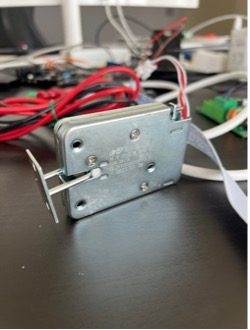
\includegraphics[height=7cm]{F1_lockerSlot.jpg}
    \captionsetup{justification=centering, singlelinecheck=false}    
    \caption{Een locker slot.}
    \label{fig:lockerSlot}
\end{figure}}

\begin{figure}[h]
    \centering
    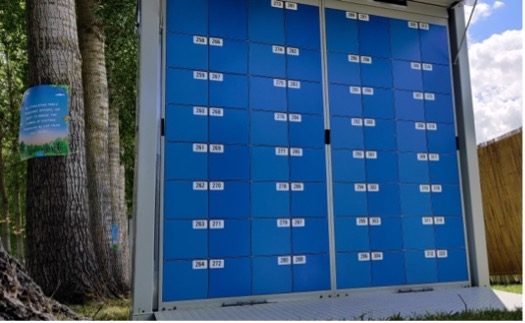
\includegraphics[height=6cm]{F2_lockerUnit.jpg}
    \captionsetup{justification=centering, singlelinecheck=false}    
    \caption{Reële weergave van een locker unit.}
    \label{fig:lockerUnit}
\end{figure}

\begin{figure}[h]
    \centering
    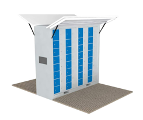
\includegraphics[height=7cm]{F3_lockerUnit2.png}
    \captionsetup{justification=centering, singlelinecheck=false}    
    \caption{Een uitgetekende weergave van een locker unit.}
    \label{fig:lockerUnit2}
\end{figure}}

\section{Hoe is een QR-code opgebouwd}%
\label{sec:opbouwQR-code}

Een QR-code is een machinaal leesbaar optisch label met informatie over het bijhorende product \autocite{Chang2014}. In deze context wordt het product als toegangscode gebruikt. QR-code staat voor Quick Response code en is een matrix van de welbekende streepjes code \autocite{Tiwari2016}. Het is een tweedimensionale code die informatie zoals tekst, URL of andere data bevat  \autocite{Shin2012} \autocite{Baharav2013}. In ons geval is het dus informatie die toebehoort bij een overeenkomstige locker. De QR-code is zodanig ontworpen dat ze door een smartphone uitgelezen kan worden aan hoge snelheden \autocite{Tiwari2016}. Dit maakt het optimaal als de QR-code gebruikt wordt als toegangscode \autocite{Narang2012}. De grootte van de QR-code kan aangepast worden naarmate de hoeveelheid data die hierin gestockeerd moet worden \autocite{Tiwari2016}. 
\\
Een QR-code wordt opgebouwd en voorgesteld als een vierkant \autocite{Fujita2011}. Hierrond bevindt zich een witte omranding. Dit vormt een contrast zodat de QR-scanner minder moeite heeft om de oppervlakte uit te lezen \autocite{Wang2015}. Dit is 1 van de 7 cruciale eigenschappen. Plaats markeringen zijn aanwezig om de scanner een duiding te geven hoe de code is gepositioneerd. Uitlijnmarkeringen hebben eveneens dezelfde functie maar deze zijn meer van toepassing bij grote QR-codes. De QR-code bevat timing patronen, dit zijn lijnen die de scanner vertellen hoe groot de data matrix is. De twee belangrijkste elementen van een QR-code zijn gegevens en foutcorrectiesleutels. Hierin zit de data gecapteerd inclusief de informatie hoe het algoritme moet omgaan met fouttolerantie \autocite{Tiwari2016}  \autocite{Petrova2016}  \autocite{Li2018}). Op figuur \ref{fig:voorstellingQR} zie je een visuele weergave. 
De fouttolerantie is doorslaggevend indien de QR-code gebruikt wordt als toegangscode \autocite{Tiwari2016}.  De fouttolerantie kan ingesteld worden door configuratie toe te passen. Het kan ingesteld worden op vier levels beginnend bij fouttolerantie van 7\% tot 30\% \autocite{Tiwari2016}.

\begin{figure}[h]
    \centering
    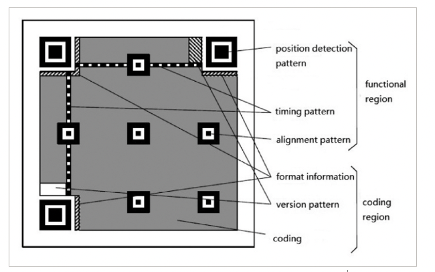
\includegraphics{F4_voorstellingQrCode.png}
    \captionsetup{justification=centering, singlelinecheck=false}    
    \caption{Een technische voorstelling van een QR-code.}
    \label{fig:voorstellingQR}
\end{figure}}

De voordelen van de QR-codes vormen een duidelijk beeld waarom Lockit Rentals voor deze technologie gekozen heeft. Niet enkel naar functionaliteit en flexibiliteit toe maar eveneens is het een makkelijk traceerbare tool. Bij verkoop van QR-codes kan men een overzicht opmaken hoeveel QR-codes er effectief gegenereerd zijn. Op basis van deze gegevens kunnen verkoopcijfers makkelijk berekend worden. 

De kans op diefstal wordt ook alsmaar kleiner als de toegangscode bestaat uit elementen die niet waarneembaar zijn \autocite{Baharav2013}. Hoe minder de persoon in kwestie weet over de code hoe moeilijker deze is om door te geven aan anderen ook al is het niet hun intentie.
\newpage
\subsection{Opbouwen van QR-codes voor verkoop}%
\label{sec:opbouwQR-codeVerkoop}

De applicatie kan meerdere versies van QR-codes genereren elk met hun eigen doel en eigenschappen. Zo bestaan er QR-codes die de software automatisch updaten of een universele QR-code die automatisch alle lockers kan openen. Deze functionaliteit wordt gebruikt voor de lockers te controleren na elk evenement. 

Hoewel een QR-code een standaard grafische voorstelling is, kan de grootte van een code verschillen. Wanneer een code groter is, ontstaat er meer witruimte tussen de pixels \autocite{Li2018}. Hierdoor kan de camera de code makkelijker en sneller scannen \autocite{Karrach2020}. Ook de foutcorrectie zorgt ervoor dat de resolutie vergroot zal worden. Hoe groter de resolutie van de QR-code hoe meer data gestockeerd kan worden \autocite{Chow2016}. 

\subsubsection{De reservatie voor een toegangscode van een locker}%
\label{sec:opbouwQR-codeVerkoop1}

\textit {De toelichting die hieronder weergeven wordt, is een vereenvoudigde voorstelling van de effectieve implementatie. Dit onderdeel van de toepassing is niet het hoofdonderwerp van deze bachelorproef, op deze analogie wordt niet verder ingegaan.}

\vspace{7}
De gegevens van de klant worden opgevraagd als hij/zij een QR-code wenst te kopen. Aan de hand van deze gegevens wordt er een gebruikersaccount automatisch aangemaakt en worden de gegevens bijgehouden \ref{lst:ophalenUser}. Deze aanpak maakt het mogelijk om nadien een koppeling te leggen tussen lockernummer en gebruiker. De reservatie en tot stand brengen van een QR-code zijn twee aparte concepten.
\begin{lstlisting}[caption={Ophalen de zopas aangemaakte gebruiker zijn gegevens indien hij in het huur proces terecht gekomen is.}, label={lst:ophalenUser}]
    /**
    * Get the user auth uid
    */
    const userAuthUid: string | undefined = context.auth?.uid;
    
    if (!userAuthUid) {
        functions.logger.error('No authenticated user was found', { data: data });
        throw new functions.https.HttpsError(
        'invalid-argument',
        'Something went wrong authenticating your device.'
        );
    }
    
    /**
    * If this user is registerd, get his info
    */
    let user: User;
    if (context?.auth?.token.email) {
        const userd = await db.collection('users').doc(userAuthUid).get();
        user = userd.data() as User;
    }
\end{lstlisting}

Bij het huurproces van een locker moet een huurder het festival aanduiden waar hij/zij de locker wil huren. Niets sluit uit dat de lockers operationeel zijn op twee verschillende locaties. Daarna heeft de huurder de keuze om het formaat te selecteren en als deze optie beschikbaar is hoelang de huurtijd zal zijn. Echter is het verstrijken van deze details over het geselecteerde evenement noodzakelijk voor de opbouw van de QR-code. De QR-code wordt gegenereerd op basis van de beschikbare lockers die aanwezig zijn op het geselecteerde evenement \ref{lst:ophalenEventInfo}.

\begin{lstlisting}[caption={Het informatie ophalen van de geselecteerde locatie. Aan de hand van geselecteerde evenement kan er gegevens uit de databank gehaald worden.}, label={lst:ophalenEventInfo}]
    /**
    * Get more info about the shop
    */
    const shopSnap = await db.collection('shop').doc(data.shopId).get();
    const shop: Shop = shopSnap.data() as Shop;
    
    /**
    * Check if selected option is active in shop
    */
    if (!shop.activeOptions?.find((o) => o.optionId === data.optionId)) {
        functions.logger.error(
        'Attempting reservation creation for non-active option',
        { data: data }
        );
        throw new functions.https.HttpsError(
        'invalid-argument',
        'This option is not yet active.'
        );
    }
    
    /**
    * Get more info about the option and location
    */
    const optionSnap = await db
    .collection('shop')
    .doc(data.shopId)
    .collection('options')
    .doc(data.optionId)
    .get();
    const option: ShopOption = optionSnap.data() as ShopOption;
    
    if (!option) {
        functions.logger.error('Can not find option for id', { data: data });
        throw new functions.https.HttpsError(
        'invalid-argument',
        'Something went wrong.'
        );
    }
    
    const locationSnap = await db
    .collection('shop')
    .doc(data.shopId)
    .collection('locations')
    .doc(option.location)
    .get();
    const location: ShopLocation = locationSnap.data() as ShopLocation;
    
    if (!location) {
        functions.logger.error('Can not find location for id', { data: data });
        throw new functions.https.HttpsError(
        'invalid-argument',
        'Something went wrong.'
        );
    }
\end{lstlisting}

Op voorwaarde dat de gebruiker informatie geldig is en er nog een locker beschikbaar is, zal er een reservatie aangemaakt worden en meteen bewaard worden in een databank. Het code die hiervoor verantwoordelijk is wordt afgebeeld in listing \ref{lst:aanmakenReservatie}.

\begin{lstlisting}[caption={De creatie van een reservatie voor het huren van een locker. Deze reservatie wordt bijgehouden in de databank}, label={lst:aanmakenReservatie}]
    /**
    * Create the reservation
    */
    const createdReservationRef = db
    .collection('shop')
    .doc(data.shopId)
    .collection('reservations')
    .withConverter(converter<ShopReservation>())
    .doc();
    
    await transaction.set(createdReservationRef, {
        id: createdReservationRef.id,
        /**
        * Here we decide if the reservation should be filled asap without payment or if a payment is needed
        */
        status: determineReservationStatus(option, data, context, user),
        customerAuthId: userAuthUid,
        customerOrigin: context.rawRequest.headers.referer,
        customerEmail: data.customerEmail,
        customerName: data.customerName,
        customerPhone: data.customerPhone,
        lockerType: data.lockerType,
        shopId: shopSnap.id,
        shopName: shop.name,
        shopAvatar: shop.avatar,
        optionColor: option.color,
        optionId: optionSnap.id,
        optionLocationId: locationSnap.id,
        optionLocationName: location.name,
        optionName: option.name,
        optionPeriodFrom: option.periodFrom,
        optionPeriodTo: option.periodTo,
        optionType: option.optionType,
        priceToPay: option.pricePerType[data.lockerType],
        manual: !!data.manual,
        reservationCreated: moment().unix(),
    });
    
    return Promise.resolve(createdReservationRef);
});
\end{lstlisting}

\subsubsection{Het betalingsverzoek voor een toegangscode van een locker}%
\label{sec:opbouwQR-codeVerkoop12}

Wanneer de databank een nieuwe reservatie constateert, word er een trigger uitgevoerd. Een trigger is een procedure die verplicht uitgevoerd wordt als een welbepaalde tabel een aanpassing ondergaat \autocite{documentation}. In dit geval is het de tabel ‘reservations’. Deze trigger zal een methode aanroepen om het betalingsverzoek te gecreëeren. 
De logistieke medewerkers kunnen huurders helpen indien hun QR-code te hard beschadigd is of als ze hun toegangscode tot de locker verloren zijn. Bij het aanmaken van toegangscodes bij logistieke medewerkers verloopt het proces op een alternatieve wijze.  Deze springen over het betalingsproces en verwerven direct een geldige QR-code. Zonder de aangemaakte betaling veld in de databank op te slaan.  \ref{lst:aanmakenBetaling}

\begin{lstlisting}[caption={Valideert of er een betaling van toepassing is. Indien nodig creëert het een betaling en bewaard deze in de databank}, label={lst:aanmakenBetaling}]
    /**
    * No action is needed but to move the status along
    */
    if (createdReservation.status === ReservationStatus.NO_PROVIDER_NEEDED) {
        await snap.ref.update({
            status: ReservationStatus.OPEN,
        });
    }
    
    /**
    * A payment is needed
    */
    if (createdReservation.status === ReservationStatus.WAITING_FOR_PROVIDER) {
        const mollieApiKey = process.env.MOLLIE_API_KEY || '';
        
        const mollie = await createMolliePayment(mollieApiKey, createdReservation);
        
        /**
        * Create the payment
        */
        const paymentRef = db
        .collection('shop')
        .doc(createdReservation.shopId)
        .collection('payments')
        .withConverter(converter<ShopPayment>())
        .doc();
        
        await paymentRef.set({
            id: paymentRef.id,
            reservationId: createdReservation.id,
            customerEmail: createdReservation.customerEmail,
            customerName: createdReservation.customerName,
            customerPhone: createdReservation.customerPhone,
            lockerType: createdReservation.lockerType,
            optionColor: createdReservation.optionColor,
            optionId: createdReservation.optionId,
            optionLocationName: createdReservation.optionLocationName,
            optionName: createdReservation.optionName,
            priceToPay: createdReservation.priceToPay,
            shopName: createdReservation.shopName,
            status: ShopPaymentStatus.PENDING,
            provider: PaymentProvider.MOLLIE,
            mollieData: {
                id: mollie.id,
            },
        });
\end{lstlisting}

De tool Mollie is een online betalingsservice deze wordt gehanteerd om de betalingen succesvol af te ronden \autocite{docs2023}. Gelijktijdig met de betaling wordt er een interne teller bijgehouden zodat deze locker geblokkeerd wordt voor andere kopers. Als de betaling niet succesvol is, wordt de locker terug vrijgegeven na een bepaalde periode. De betaling word aangemaakt met de gekende informatie over de gewilde locker \ref{lst:aanmakenBetalingMollie}.

\begin{lstlisting}[caption={Mollie betaling aanmaken met nodige data.}, label={lst:aanmakenBetalingMollie}]
    async function createMolliePayment(
    mollieApiKey: string,
    reservation: ShopReservation
    ): Promise<Payment> {
        const mollieClient = createMollieClient({
            apiKey: mollieApiKey,
        });
        return mollieClient.payments.create({
            amount: {
                value: reservation.priceToPay.toFixed(2),
                currency: 'EUR',
            },
            description:
            reservation.shopName +
            ' | ' +
            reservation.optionName +
            ' | ' +
            reservation.lockerType,
            redirectUrl: reservation.customerOrigin + 'reservations/' + reservation.id,
            webhookUrl:
            reservation.customerOrigin?.includes('localhost') ||
            reservation.customerOrigin?.includes('test')
            ? 'https://europe-west2-lockit-testing.cloudfunctions.net/mollieWebhook'
            : 'https://europe-west2-lockit-435cd.cloudfunctions.net/mollieWebhook',
            metadata: {
                shop: reservation.shopName,
                reservation: reservation.id,
                option: reservation.optionName,
                location: reservation.optionLocationName,
                lockerType: reservation.lockerType,
                customer: reservation.customerName,
                customerEmail: reservation.customerEmail,
                customerPhone: reservation.customerPhone,
            },
        });
    }
    \end{lstlisting}

Bij correcte betaling van de klant, zal de applicatie de desbetreffende creatiemethode aanspreken om dergelijke QR-code te genereren. Deze QR-code bevat een random geselecteerde locker nummer inclusief een tijdspanne waarin de toegangscode geldig is. De status van de reservatie die zich al in de databank bevindt word aangepast. Hierdoor weet heel de applicatie dat die bepaalde reservatie betaald is \ref{lst:voltooidebetaling}.


\begin{lstlisting}[caption={Voltooide betaling roept de creatie QR-code methode op. Hierbij gebeurt een status update van de vooraf aangemaakte reservatie.}, label={lst:voltooidebetaling}]
    await db.runTransaction(async (transaction) => {
        /**
        * Find a valid available locker
        * Because we can only compare 10 units with the firestore "IN" clause we have to split up
        */
        
        if (!location?.units) {
            throw new Error('No units assigned');
        }
        
        const availableLockerSnap = await getRandomLockerAvailable(
        transaction,
        db,
        reservation.lockerType,
        location?.units
        );
        if (!availableLockerSnap) {
            logger.error('no-open-locker-found', {
                reservation: reservation,
                option: option,
                location: location,
            });
            throw new Error('NO Open lockers found');
        }
        
        const generatedCode = await generateQrCodeWithRecordOnTransaction(
        transaction,
        {
            lockerNumber: availableLockerSnap.data().number,
            start: option?.periodFrom as number,
            end: option?.periodTo as number,
            color: option?.color as string,
            image: reservation?.shopAvatar,
            location: location?.name,
            periodName: option?.name as string,
            name: reservation?.shopName,
        }
        );
        
        /**
        * update current reservation
        */
        await transaction.update(reservationSnap.ref, {
            status: ReservationStatus.FILLED,
            accessCode: generatedCode,
            lockerNumber: availableLockerSnap.data().number,
        });
\end{lstlisting}


\subsubsection{Creatie QR-code na succesvolle betaling.}%
\label{sec:opbouwQR-codeVerkoop123}

Om de QR-code te tonen op de mobiele applicatie hebben we componenten nodig om de gegenereerde QR-code visueel te tonen zoals op figuur \ref{fig:qrCodeGebruiker} of figuur \ref{fig:qrCodeAdmin}. Hierdoor kan de koper zowel de code scannen op zijn/haar telefoon als op een afgedrukt kaartje \autocite{Chow2016}.

\begin{figure}[h]
    \centering
    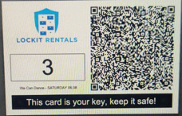
\includegraphics{F5_qrcodeKoper.png}
    \captionsetup{justification=centering, singlelinecheck=false}    
    \caption{Een voorbeeld van een QR-code die gekocht is door een gebruiker voor specifieke lockertoegang op een evenement.}
    \label{fig:qrCodeGebruiker}
\end{figure}}

\begin{figure}[h]
    \centering
    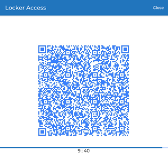
\includegraphics{F6_qrcodeAdmin.png}
    \captionsetup{justification=centering, singlelinecheck=false}    
    \caption{Een voorbeeld van een QR-code die gegeneerd is door een logistieke medewerker met de juiste bevoegdheden voor specifieke lockertoegang op een evenement.}
    \label{fig:qrCodeAdmin}
\end{figure}}

\newpage
Aangezien de generatie van een QR-code dat voorgesteld is als afbeelding wat front-end matige materie is, zal onderstaande code de werking weergeven \ref{lst:qrComponent}. 

\begin{lstlisting}[caption={Typescript code voor een visuele QR-code aan te maken}, label={lst:qrComponent}]
    await db.runTransaction(async (transaction) => {
        export class QrcodeViewerComponent implements OnInit {
            activeQrCode: string = 'EjIQT51wpdf6Is1r+R5+mt8aU0waHVKVK9lzvhXRV4w=';
            
            @Input() data: string = '';
            @Input() deCryptedData: QrCodeData = QrCodeData.createEmptyQrCodeData();
            
            secondsLeft$: Observable<number> = new BehaviorSubject(0);
            
            private qr_opts = {
                errorCorrectionLevel: 'H',
                type: 'image/jpeg',
                quality: 1,
                margin: 10,
                color: {
                    dark: '#3880ff',
                },
            };
            
            constructor(private modalController: ModalController) {
                this.secondsLeft$ = interval(1000).pipe(
                filter(
                () => !!this.deCryptedData.validFrom && !!this.deCryptedData.validTo
                ),
                map(() => this.deCryptedData.getSecondsLeftUntilEnd())
                );
            }
            
            ngOnInit(): void {
                qrcode
                .toDataURL(this.data, this.qr_opts as QRCodeToDataURLOptions)
                .then((qr) => {
                    this.activeQrCode = qr;
                });
            }
            
            dismissModal() {
                this.modalController.dismiss();
            }
        }
    \end{lstlisting}

Lijn 3: De variabele ‘activeQrCode’ van type string is de publieke sleutel die wordt gebruikt om de QR-code te ontcijferen. \\
Lijn 10 – 18: De ingestelde eigenschappen die gedefinieerd zijn om de QR-code aan te maken. Men kan de code naar zijn behoefte configureren \autocite{Sutheebanjard2010}. Een belangrijke waarde is hierbij de ‘ErrorCorrectionLevel’, deze veranderd doorheen de applicatie op basis waar de QR-code afgebeeld moet worden. Hierdoor mag de QR-code voor 30\% beschadigd of gescheurd zijn. De scanner zal alsnog de afbeelding succesvol kunnen detecteren \autocite{Tiwari2016}. \\
Lijn 29– 35: De tool die gehanteerd wordt om de QR-code te genereren is de bibliotheek ‘qrcode’ \autocite{pypi2023}. 

\newpage
\section{Het incrypteren en decrypteren van QR-codes is een QR-code opgebouwd}%
\label{sec:encryptQR-code}

Eerder in de werking van de QR-units is de validatie NaCL genaamd ‘Networking And Cryptography Library’ aan bod gekomen \autocite{Bernstein}. De hoofdfunctionaliteit van de recente software bibliotheek is het vercijferen en ontcijferen van bestanden. Het biedt alle kernbewerkingen aan die betrekking hebben om cartografische benodigdheden op hoger niveau te bouwen \autocite{Bernsteina}.

In de applicatie van Lockit Rentals is er gebruik gemaakt van TweetNaCl.js. TweetNaCl is een compacte versie van de implementatie bibliotheek NaCL \autocite{Bernstein2014} \autocite{Bernsteinb}. Deze bevat verschillende encryptie en onderteken algoritmes op basis van ed25519 \autocite{Bernstein2011}. \\
Ed25519 gebruikt het onderliggende algoritme Curve25519. Curve25519 is vooral ontworpen om snel, efficiënt en op een effectieve manier sleutelwisseling te gaan uitvoeren. Zo worden beide partijen op de hoogte gesteld van hun gezamenlijke sleutel \autocite{Bernstein2006}. Ed25519 aan de andere kant heeft andere prioriteiten. Deze zal op een betere en sneller manier algoritmen uitvoeren specifiek voor digitale ondertekeningen gaan uitvoeren. \autocite{Bernstein2011}. \\
In het kader van smart locker systemen wordt de encryptie gebruikt om de QR-codes digitaal te ondertekenen. De reden van gebruik ligt bij een voordeel van TweetNaCL.js die heel voordelig uitkomt bij de gegeven implementatie. Het heeft namelijk als voordeel dat deze beschikt over kleine onderteken sleutels ook wel ‘signatures’ genoemd \autocite{Bernstein2011}. Hoe minder gestockeerde data in de QR-code kleiner de afdruk is van de code \autocite{Chow2016}.

Deze term van algoritme wordt ‘signing’ genoemd. Het algoritme zal verifiëren of de data in de QR-code onveranderd blijft gedurende het gehele proces \autocite{Bernsteinb}. Het proces begint bij het tot stand brengen van een QR-code tot aan het scannen ervan.

De documentatie website van TweetNaCl.js laat de verschillende encryptie tool gratis uitproberen \autocite{Bernsteinb}. Een concreet voorbeeld hieronder geeft duiding hoe een specifiek bericht ondertekend kan worden. Hieruit kan aangetoond worden of het bericht al dan niet is aangepast na de creatie \autocite{Bernstein2014}.

\subsubsection{Uitgewerkt voorbeeld van digitale ondertekening op een standaard bericht.}%
\label{sec:voorbeeldDigitaleSigning}

Bij het ondertekenen van een bericht heeft het algoritme nood aan één geheime sleutel evenals één publieke sleutel
\ref{fig:privatePublicKey}. De geheime sleutel wordt gebruikt om nadien de versleutelde code te decrypteren.

\begin{figure}[h]
    \centering
    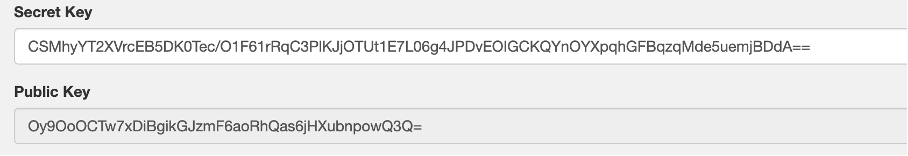
\includegraphics{F7_privatePublicKeys.png}
    \captionsetup{justification=centering, singlelinecheck=false}    
    \caption{De publieke en private sleutel voor encryptie aan de hand van TweetNaCL.js.}
    \label{fig:privatePublicKey}
\end{figure}}
 \newpage
In deze illustratie wordt een bericht dat afgebeeld staat hieronder \ref{fig:encryptionBericht} meegeven met de functie van TweetNaCl. Met als doel dit bericht te laten ondertekenen aan de hand van de geheime sleutel.

\begin{figure}[h]
    \centering
    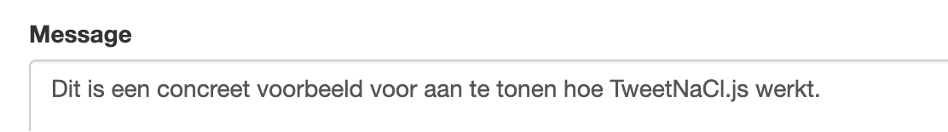
\includegraphics{F8_messageEncryption.png}
    \captionsetup{justification=centering, singlelinecheck=false}    
    \caption{Het bericht dat cryptisch ondertekend moet worden aan de hand van TweetNaCL.js.}
    \label{fig:encryptionBericht}
\end{figure}}

Bij ondertekening van dit bericht ontstaat er een unieke handtekening  \ref{fig:signatureQrcode} als zijnde een tekenreeks. Aan de hand van deze code kan de ontvanger verifiëren dat het bericht gedurende het proces niet gewijzigd is.

\begin{figure}[h]
    \centering
    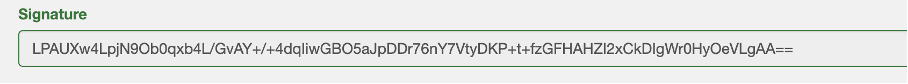
\includegraphics{F9_signature.png}
    \captionsetup{justification=centering, singlelinecheck=false}    
    \caption{De gegenereerde digitale handtekening aan de hand van TweetNaCL.js}
    \label{fig:signatureQrcode}
\end{figure}}

Om na te gaan of dit bericht zijn oorspronkelijke data bevat zal de functie ‘verify’ opgeroepen worden. In het geval dat dit bericht niet in oorspronkelijke status bevindt, zal de functie een foutboodschap retourneren \ref{fig:verifyFailed}. Als de methode geen foutboodschap weergeeft, kan men concluderen dat deze data origineel is \autocite{Bernstein2014}. Zoals word weergegeven in figuur \ref{fig:verified}.

\begin{figure}[h]
    \centering
    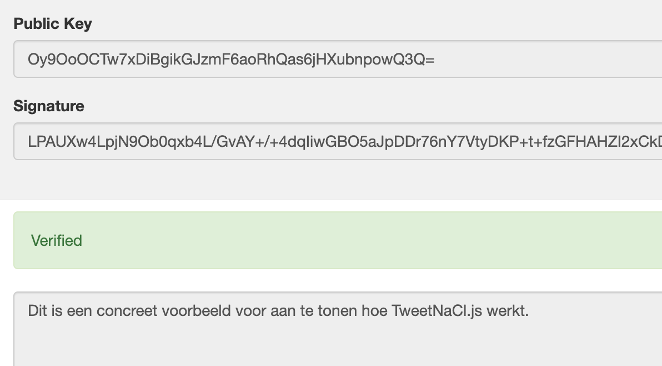
\includegraphics{F10_verified.png}
    \captionsetup{justification=centering, singlelinecheck=false}    
    \caption{Bewijs dat bericht zich in originele  staat bevindt.}
    \label{fig:verified}
\end{figure}}

\begin{figure}[h]
    \centering
    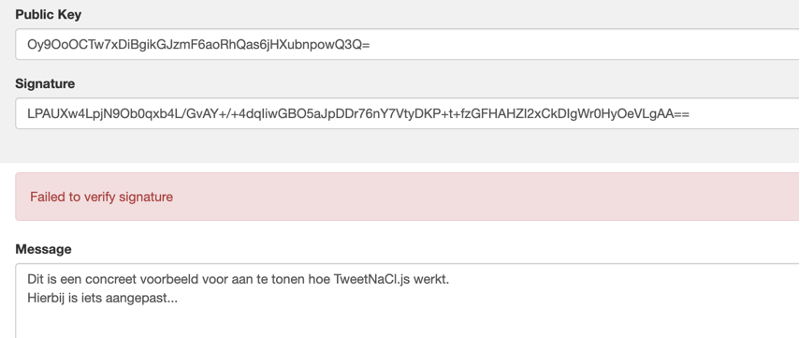
\includegraphics{F11_failedVerify.png}
    \captionsetup{justification=centering, singlelinecheck=false}    
    \caption{Bewijs dat bericht zich in geen originele  staat bevindt.}
    \label{fig:verifyFailed}
\end{figure}}
\\
\newpage
\newpage
\subsubsection{Uitgewerkt voorbeeld van digitale ondertekening op een aangemaakte QR-Code.}%
\label{sec:voorbeeldDigitaleSigningQRCode}

Bij de implementatie van deze smart locker technologie is het bericht dat standaard meegegeven wordt de QR-code data van type \ac{JSON} object. Deze kan niet ondertekend worden zolang het niet geconverteerd wordt naar een tekstueel gegeven. De omvorming van een \ac{JSON} object naar een string wordt verwerkt door de functie ‘deCodeBase64’. Deze functie zal de reeks decoderen terug naar het oorspronkelijke binair formaat \autocite{Josefsson2006}.



\begin{lstlisting}[caption={Data object met de naam smallItem bevat de essentiele data om een locker te openen.}, label={lst:essentieleQrdata}]
    export async function generateQrCodeWithRecord(qrData: {
        lockerNumber: any;
        start: number;
        end: number;
        color: string;
        image: string;
        location: string;
        name: string;
        periodName: string;
    }) {
        const smallItem = convertToSmallPayload(
        qrData.lockerNumber,
        qrData.start,
        qrData.end
        );
\end{lstlisting}

Lijn 11 - 15 \ref{lst:essentieleQrdata} :  De data die essentieel is om toegang te hebben tot de locker wordt gedefinieerd als de variabele ‘smallItem’. Aangezien de eigenschappen zoals kleur, locatie en afbeelding niets te maken heeft met de scanfunctie van de QR-unit. Word deze informatie hiervan gescheiden.

De functie ‘NaCL. Sign()’ aanvaardt twee parameters \ref{lst:encryptionCode}. In de eerste plaats nemen we de locker informatie op. Deze informatie beschikt over de locker nummer, creatiedatum QR-code en verval datum QR-code \ref{lst:essentieleQrdata}. Het is noodzakelijk dat het tekstbericht het juiste type is daarom wordt ‘smallItem’ omgezet naar een JSON object en daarna geconverteerd naar byte door de functie ‘decodeUTF8()’. Vervolgens heeft de functie een geheime sleutel nodig om de ondertekening te kunnen uitvoeren.

\begin{lstlisting}[caption={Digitale ondertekening van QR-code data.}, label={lst:encryptionCode}]
    const data = nacl.sign.detached(
    decodeUTF8(JSON.stringify(smallItem)),
    decodeBase64(
    'Hier komt de private key.'
    )
    );
    \end{lstlisting}


Door de twee gecreëerde objecten, QR-data en de digitale handtekening samen te voegen ontstaat er een \ac{JSON} object genaamd ‘createdCode’ \ref{lst:createCode}. De code wordt achteraf omgevormd naar een tekstueel formaat.

\begin{lstlisting}[caption={Samenstellen van object, locker informatie en verificatie code.}, label={lst:createCode}]
    const createdCode = Buffer.from(
    JSON.stringify({ d: smallItem, v: encodeBase64(data) })
    ).toString('base64');
\end{lstlisting}

\newpage
\subsubsection{Uitgewerkt voorbeeld van de verifieer functie op de een aangemaakte QR-Code.}%
\label{sec:controleaangemaakteQRcode}

Als illustratie maken we een QR-code aan op de applicatie die bestemd is voor locker nummer één. De geldigheidsduur van de code is tien minuten. Het request kan onderschept worden om zo de data te analyseren. We beelden het object af in figuur \ref{fig:dataobjectQR}.

\begin{figure}[h]
    \centering
    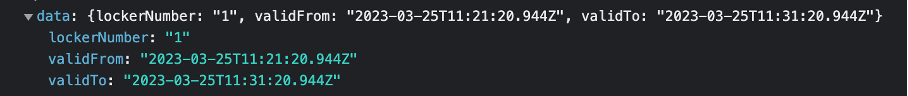
\includegraphics{F12_requestQrCode.png}
    \captionsetup{justification=ce/brntering, singlelinecheck=false}    
    \caption{Het data object bij de creatie van locker nummer 1 als logistieke medewerker. Deze heeft een tijdspanne van tien minuten.}
    \label{fig:dataobjectQR}
\end{figure}}

Als we dieper in de materie duiken is de aangemaakte code zichtbaar als antwoord op het creatieverzoek. De tekstuele code voorgesteld als base64 string ziet er als volgt uit: \\
 “eyJkIjp7Im4iOiIxIiwiZiI6MTY3OTc0MzIyMSwidCI6MTY3OTc0Mzg4MX0sInYiOiJLYT\\
 cwTmg4WUo3RlY0NmNiKythNlN3b21vczFFVURiQlpxajl2ZDhpNlNUWGZHU003eVN\\
 2ZGw0ZEs5WGp3clpyVnNV RlpHR3E3RVJGSlJQR09HTkxEdz09In0=".
 
\vspace{7}

Deze code wordt achter een vaste ingestelde URL geplaatst zodanig dat de QR-code gemakkelijk gedeeld kan worden. Het delen of doorsturen van een QR-code is een eenvoudig proces voor de huurder \ref{lst:shareQR}. Bij het delen van een QR-code wordt er een link gecreëerd dat verwijst naar de web applicatie van Lockit Rentals \ref{lst:createQRLink}. De applicatie zal de base64 string ontvangen en de link ontcijferen om zo een afbeelding van de QR-code genereren.

\begin{lstlisting}[caption={Het doorsturen van een QR-code in de vorm van een link.}, label={lst:shareQR}]
    handler: async () => {  
        await Share.share({
            title: 'Have access to my locker',
            text: 'Hi there, I want to share my locker with you. Open this link!',
            url: this.constructQRCodeData(qrData as string),
            dialogTitle: 'Share your locker with friends',
        });
\end{lstlisting}

\begin{lstlisting}[caption={De manier hoe de link van de QR-code is gestructureerd.}, label={lst:createQRLink}]
    constructQRCodeData(encryptedPart: string): string {
        return location.protocol + '//' + location.host + '/?code=' + encryptedPart;
    }
\end{lstlisting}

Op de figuur \ref{fig:decoderBase64ToJson} wordt een base64 van het type string omgevormd en ontcijferd  naar een tekstuele vorm. Hiervoor kan er gebruik gemaakt worden van gratis online tools. Om het base64 formaat te ontcijferen bestaat er een online decoder \autocite{base64decode}. 


\begin{figure}[h]
    \centering
    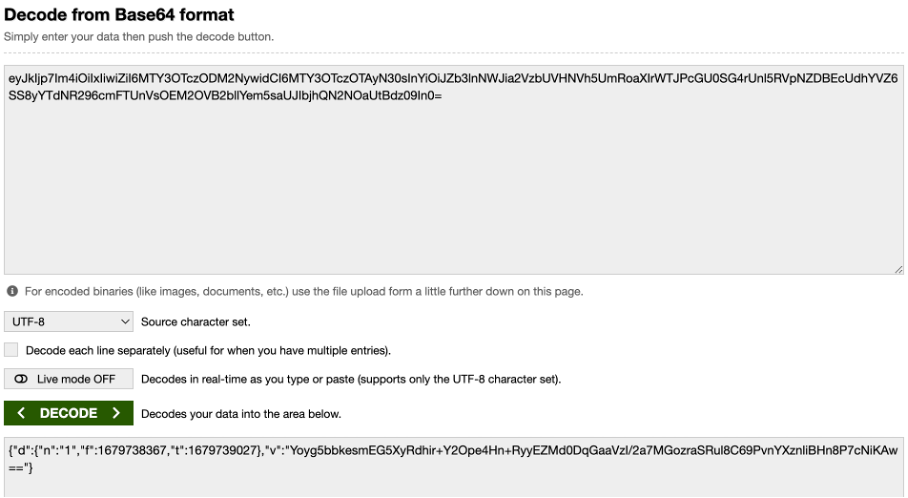
\includegraphics{F13_decoderbase64.png}
    \captionsetup{justification=ce/brntering, singlelinecheck=false}    
    \caption{De manier waarop een base64 string geconverteerd word naar een \ac{JSON} aan de hand van een online decoder.}
    \label{fig:decoderBase64ToJson}
\end{figure}}

Voor eenvoud van het illustratief voorbeeld vormen we dit om naar een gestandaardiseerd \ac{JSON} object \autocite{Concept}. Het geformatteerd \ac{JSON} object geeft een visueel beeld van de twee variabelen in de genereerde QR-code. Het visueel beeld word afgedrukt in de figuur \ref{fig:formattedJsonData}.

\begin{figure}[h]
    \centering
    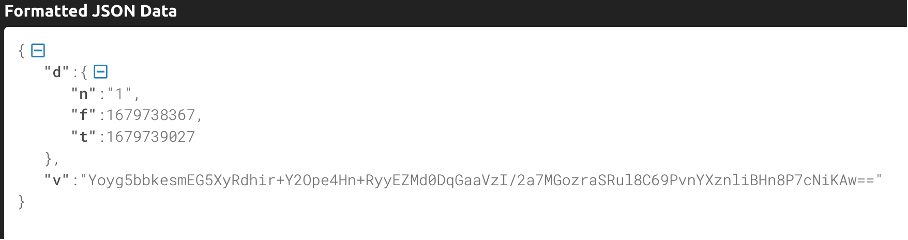
\includegraphics{F14_formattedJsonData.png}
    \captionsetup{justification=ce/brntering, singlelinecheck=false}    
    \caption{Het JSON object converteren naar een gestandaardiseerde vorm.}
    \label{fig:formattedJsonData}
\end{figure}

\newpage
Om de data te controleren wordt de functie ‘verify’ aangeroepen \ref{lst:verifyMethode}, deze heeft 3 parameters nodig. Als eerste het object waarin de QR-code data zit. Vervolgens geven we de verificatie code mee. De publieke sleutel is de laatste parameter om te decrypteren.


\begin{lstlisting}[caption={De controle van QR-code data met de TweetNaCL.js verifieer functie.}, label={lst:verifyMethode}]
    // Check if the object validates
    if (
    !nacl.sign.detached.verify(
    decodeUTF8(JSON.stringify(obj.d)),
    decodeBase64(obj.v),
    decodeBase64(publicKey)
    )
    ) {
        return new Error();
    }
\end{lstlisting}

Als data zijn originele vorm heeft aangehouden, zal de functie geen foutboodschap geven zoals in figuur \ref{fig:qrdataVerified}. Bij onveranderlijke data kan er van uitgegaan worden dat de QR-code informatie niet aangepast is doorheen het proces \autocite{Bernsteinb}. 

\begin{figure}[h]
    \centering
    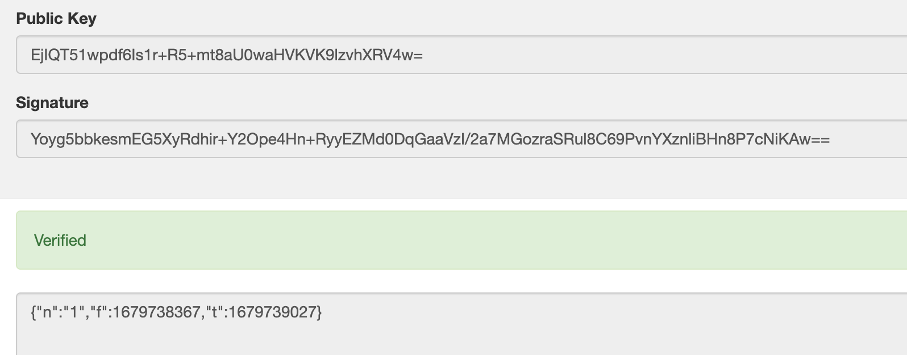
\includegraphics{F15_qrcodeVerified.png}
    \captionsetup{justification=ce/brntering, singlelinecheck=false}    
    \caption{De QR-code data dat vanaf de aanmaak tot de verifieer  functie ongewijzigd is gebleven.}
    \label{fig:qrdataVerified}
\end{figure}

\newpage

\section{De werking van een smart locker systeem.}%
\label{sec:WerkingUnits}

Een stabiele werking van het smart locker systeem is cruciaal aangezien hier het volledige business model op draait. Figuur \ref{fig:schemaWerkingUnit} is een schematische voorstelling hoe de software in aanraking komt met de hardware. Dit door middel van de QR-code die dient als toegangscode.

\begin{figure}[h]
    \centering
    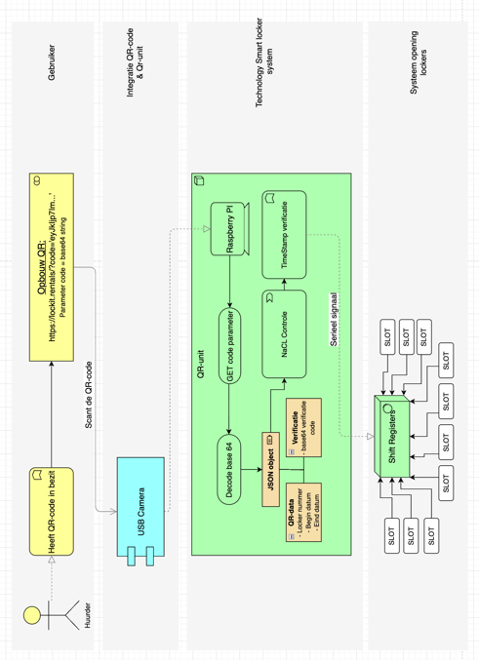
\includegraphics{F16_schemaWerking.png}
    \captionsetup{justification=ce/brntering, singlelinecheck=false}    
    \caption{Een schematische voorstelling  hoe een QR-unit operationeel te werk gaat.}
    \label{fig:schemaWerkingUnit}
\end{figure}

\begin{enumerate}
    \item De QR-code die alvorens is aangemaakt wordt uitgelezen met een USB camera. De software van de camera draait rechtstreeks op de Rasberry PI. Een Raspberry PI is een kleine maar krachtige mini computer die allerlei berekeningen kan uitvoeren \autocite{Richardson2013}. De aangesloten USB camera zal de afbeeldingen renderen en opslaan in zijn geheugen.
    \item Bij het scannen van de QR-code identificeert de Raspberry PI de URL van de QR-code \autocite{Weir2012}. De applicatie heeft enkel nood aan de parameter ‘code’. Die base64 string wordt uit de link gefilterd door de URL op te splitsen \ref{lst:pythonLinkSplitting}. Eenmaal dat de base64 string gevonden is, zal dit terug geconverteerd worden naar een \ac{JSON} object. Hieruit kunnen 3 drie elementen uitgehaald worden: het lockernummer alsook het begin en eind tijdstip dat de QR-code geldig is. Deze tijdstippen worden beide voorgesteld als type Unix. Unix stelt tijdstippen op een correcte en eenvoudige wijze voor. Deze zorgen voor een makkelijke conversie tussen verschillende tijdzones en formaten \autocite{Ritchie1978}.

        \begin{lstlisting}[language=Python, caption={Python script om parameter code uit de link te halen.}, label={lst:pythonLinkSplitting}, numbers=left]
            if (!url) {
                return new Error();
            }
            const data = url.split("code=")[1]
            const obj = JSON.parse(Buffer.from(data, 'base64').toString('utf8')); 
        \end{lstlisting}

    
    \item 
    De Raspberry PI is het hart van de hardware installatie, hier bevindt zich alle logica die uitgevoerd wordt na het scannen van de QR-code. Hieronder volgt de Python implementatie dat actief is op de Raspberry PI \ref{lst:pythonPrimary}.
    
    \begin{lstlisting}[language=Python, caption={Het primaire uitvoerbare script van de QR-unit.}, label={lst:pythonPrimary}, numbers=left]
        import cv2
        import pyzbar.pyzbar as pyzbar
        from datetime import datetime, timedelta
        import requests
        import time
        
        #width = 2592
        #height = 1944
        
        camera = cv2.VideoCapture(0)
        #camera.set(3,width)
        #camera.set(4,height)
        
        
        def decodeCam(image):
            try:
                gray = cv2.cvtColor(image, cv2.COLOR_BGR2GRAY)
                barcodes = pyzbar.decode(gray, symbols=[pyzbar.ZBarSymbol.QRCODE])
                global data
                global stamp
                for barcode in barcodes:
                barcodeData = barcode.data.decode()
                barcodeType = barcode.type
                if barcodeData != data or stamp + timedelta(days=0, seconds=5) < datetime.now():
                print("["+str(datetime.now())+"] Type:{} | Data: {}".format(barcodeType, barcodeData))
                res = requests.post('http://localhost:5000/qr-code', json = {'tag': barcodeData })
                print(res)
                data = barcodeData
                stamp = datetime.now()
                return image
            except Exception as e:
                print(e)
        
        try:
        global data
        data = ""
        global stamp
        stamp = datetime.now()
        print('reading camera...', end='\r')
        frame_rate = 3
        prev = 0
        while True:
        # Read current frame
        if camera.isOpened():
            time_elapsed = time.time() - prev
            ret, frame = camera.read()
            if time_elapsed > 1./frame_rate:
                prev = time.time()
                im=decodeCam(frame)
        except KeyboardInterrupt:
        print('interrupted!')
        
    \end{lstlisting}
    Lijn 10 \ref{lst:pythonPrimary}: Het definiëren van de camera zodat hij kan gebruikt worden om de QR-code waar te nemen. \\
    Lijn 34 – 41 \ref{lst:pythonPrimary}: Een oneindige lus waarin de camera constant probeert om QR-codes te scannen. Als hij een QR-code opmerkt, zal hij deze vertalen en zal de methode ‘decodeCam’ opgeroepen worden. De gescande afbeelding die voorgesteld wordt als QR-code zal hierin meegegeven worden.\\
    Lijn 17 \ref{lst:pythonPrimary}: Cv2 is een software pakket dat visuele afbeeldingen kan laden en verwerking in de taal Python. Het pakket de resulterende grijsvariabelen verwijderen die in de invoerafbeelding zitten. Dit betekent dat als de huurder een afbeelding scant hij enkel specifieke kleuren zal overhouden. Hierdoor kan het primaire Python script verder werken met één informatiekanaal, in plaats van meerdere in geval van een kleurenafbeelding \autocite{developmentteam}.\\
    Lijn 18 \ref{lst:pythonPrimary}: PyZbar is een andere bibliotheek die instaat om de QR-codes te gaan detecteren van de grijswaardenafbeelding die zonet met Cv2 bekend zijn gemaakt \autocite{Huang2022}\\
    Lijn 21 – 30 \ref{lst:pythonPrimary}: Hierin gebeurt de decoding van de parameter code in de URL. Maar uiteraard wordt dit niet rechtstreeks gedaan. Het moet eerst nog gedecodeerd worden, aangezien de QR-code versleuteld is met encryptie. \\
    Lijn 26 \ref{lst:pythonPrimary}: De Rasberry PI zal een request sturen naar de Node.js server die rechtstreeks draait op de PI. De bijhorende code wordt hieronder \ref{lst:pytho} getoont. Deze server ontvangt een parameter waarin de QR-code data zit.\\
    
    
     \begin{lstlisting}[language=Python, caption={De node.js server die de nodige validatie zal uitvoeren en de verdere communicatie afronden.}, label=lst:pytho, numbers=left]
        router.post('/qr-code', (request, response) => {
            try {
                const decryptedData = decryptor.decrypt(request.body.tag);
                console.log(decryptedData);
                const hasErrors = validator.validate(decryptedData, Number(config.unit));
                if (hasErrors) {
                    displayError(hasErrors.errorMessage);
                    return;
                }
                expressWs.getWss('/updates').clients.forEach(function (client) {
                    client.send(JSON.stringify(decryptedData));
                });
                if (decryptedData.n) {
                    pinController.openLock(calculateExactLock(Number(decryptedData.n), Number(config.unit)));
                } else if(decryptedData.r) {
                    pinController.openRange(decryptedData.r.map(l => calculateExactLock(Number(l), Number(config.unit))))
                } else if(decryptedData.u) {
                    //universal key scanned
                    
                    .......
        
    \end{lstlisting}

    Lijn 32 \ref{lst:pythonPrimary}: Het aanroepen van een voor gedefinieerd ‘decryptor’ script. Zie code in listing \ref{lst:function} De validatie hierbij zal uitmaken of de data die in de QR-code is geplaatst nog steeds correct is.    
    \begin{lstlisting}[language=Python, caption={ De parameter genaamd ‘code’ wordt verwerkt en ontcijferd, indien de QR-data is aangepast zal het een error terug geven.}, label=lst:function, numbers=left]
        decrypt: function(url) {
            if (!url) {
                return new Error();
            }
            const data = url.split("code=")[1]
            const obj = JSON.parse(Buffer.from(data, 'base64').toString('utf8'));
            
            // Check if the object validates
            if (!nacl.sign.detached.verify(decodeUTF8(JSON.stringify(obj.d)), decodeBase64(obj.v), decodeBase64(publicKey))) {
                return new Error();
            }
            
            
            return obj.d;
        }
                    
                \end{lstlisting}
   
        Validatie functie is gebaseerd op de twee tijdspanne die aanwezig zijn in het aangemaakt \ac{JSON} object. Met deze techniek kan bekeken worden of de gescande QR-code binnen een correcte tijdspanne ligt. Niet enkel controleert hij op correcte geldigheid, ook voert de code hieronder \ref{lst:data-validator} een controle uit of de QR-code wel bij de bijpassende QR-unit hoort.
        
        \begin{lstlisting}[language=Python, caption={ Valideer functie van de gescande QR-data op geldigheid en controle om na te gaan of gescande lockernummer in QR-unit zit.}, label=lst:data-validator, numbers=left]
            const moment = require('moment');
            
            module.exports = {
                validate: function(data, unit) {
                    const now = moment(); // create a moment with the current time
                    const then = moment.unix(data.t); // create a moment with the other time timestamp in seconds
                    const delta = now.diff(then, 'milliseconds'); // get the millisecond difference
                    console.log("diff to " + delta)
                    // Check if number is in range for this unit (number is not mandatory)
                    if (data.n && (data.n < getFirstLockerNumber(unit) || data.n > getLastLockerNumber(unit))) {
                        return {errorMessage: 'Locker not in this unit'}
                    }
                    // Check if after start time
                    if (moment().isBefore(moment.unix(data.f))) {
                        return {errorMessage: "This code is not yet valid"}
                    }
                    
                    // Check if before end time
                    if (moment().isAfter(moment.unix(data.t))) {
                        return {errorMessage: "This code is expired"}
                    }
                    return false;
                }
            }
            
            
            function getFirstLockerNumber(unit) {
                return ((unit - 1) * 128) + 1;
            }
            
            function getLastLockerNumber(unit) {
                return ((unit - 1) * 128) + 128;
            }
            
        \end{lstlisting}
        
        
    Lijn 42 – 62 \ref{lst:pythonPrimary}: Op basis van de correcte originele ontcijferde data kan de server van node.js de juiste sloten aansturen. De Raspberry Pi stuurt met een serieel signaal naar de verschillende shift registers, die elk op zich verantwoordelijk zijn voor een aantal verschillende sloten aan te spreken. 
    
    
\end{enumerate}

\newpage

\section{Wat is een chatbot}%
\label{sec:chatbot}

De term chatbot is heel snel geëvolueerd doorheen de voorbije jaren. Een chatbot is een "online mens-computer dialoogsysteem met natuurlijke taal" \autocite{Jia2003}. Dit wordt gebruikt om veel systemen te ondersteunen om vragen van klanten automatische te laten beantwoorden \autocite{Adamopoulou2020}. Ze maken gebruik van artificiële intelligentie die de vraagstelling van klanten analyseren. Op basis van de benodigdheden probeert de chatbot zo goed mogelijk te helpen \autocite{Khanna2015}. Dit concept waarbij de mens de computer om een gunst vraagt, wordt ‘Human-computer interaction’ (HCI) genoemd \autocite{Adamopoulou2020}. Chatbots zijn niet enkel gebouwd om conversaties op te vangen of om mensen te entertainen. Deze zijn ook ontworpen voor leer-, informatie- en bedrijfsdoeleinden \autocite{Shawar2007}. 

\subsection{Historie van een chatbot}%
\label{sec:chatbotHistorie}

Het idee van een chatbot werd het eerst gepubliceerd in 1950 \autocite{Turing2009}. Echter bestaat de eerste chatbot genaamd Eliza nog maar sinds 1966 \autocite{Weizenbaum1966}. Deze is ontworpen aan de hand van een simpel patronen overeenkomst en een vooraf aangemaakt antwoorden patroon.  Vanaf dit moment in de geschiedenis begon de functionaliteit en de ontwikkeling van chatbot alsmaar groter te worden \autocite{Brandtzaeg2017}. Zoals getoond in de figuur \ref{fig:graphDocusChatbotAYear} volgens Scopus \autocite{Elsevier2004}, was er grote en snelle groei van interesse in chatbots, zeker na het jaar 2016 \autocite{Adamopoulou2020}.

\begin{figure}[h]
    \centering
    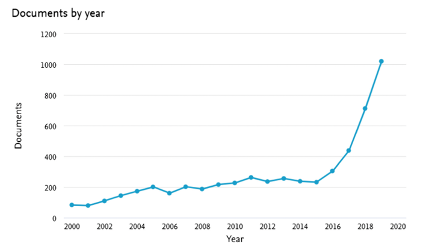
\includegraphics{F17_grafiekChatbotSearches.png}
    \captionsetup{justification=ce/brntering, singlelinecheck=false}    
    \caption{Zoek resultaten in scopus voor de termen ‘chatbot’ of ‘conversation agent’ of ‘conversational interface’ vanaf 2000 tot 2019.}
    \label{fig:graphDocusChatbotAYear}
\end{figure}


\subsection{Architectuur  van een chatbot}%
\label{sec:chatbotArchitectuur}

De start van de menselijke vraag tot een gegenereerde chatbot antwoord wordt voorgesteld als de architectuur van een chatbot. Als illustrerend voorbeeld vragen we als chatbot zijn/haar verloren QR-code op. De huurder heeft een specifieke vraag die de chatbot kan verwerken. Na het krijgen van de huurder zijn bericht zal de ‘Natural Language Understanding’ (NLUs) \autocite{Khanna2015} component de vraag analyseren en classificeren wat de gebruiker zijn intenties zijn \autocite{Tamrakar2021}. Wanneer er een duidelijk geformuleerde vraag gesteld is, kan de chatbot acties ondernemen. In het geval met de verloren QR-code zal hij een API oproep aanspreken om externe informatie op te vragen. Nadien kan de data worden vrijgegeven aan de gebruiker indien de huurder zich juist kan identificeren als het gaat om gevoelige informatie \autocite{Adamopoulou2020}. De architectuur kan voorgesteld worden op figuur \ref{fig:chatbotArchitectuur}.

\begin{figure}[h]
    \centering
    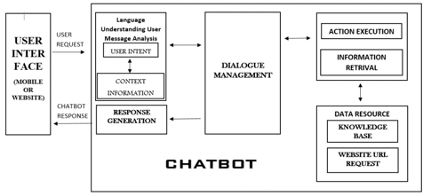
\includegraphics{F18_chatbotArchitectuur.png}
    \captionsetup{justification=ce/brntering, singlelinecheck=false}    
    \caption{Standaard architectuur van een chatbot.}
    \label{fig:chatbotArchitectuur}
\end{figure}

\subsection{Classificatie chatbots}%
\label{sec:chatbotTypes}

Chatbots kunnen geclassificeerd worden door middel van een aantal eigenschappen \ref{fig:chatbotTypes} zoals het interactie level en op welke manier de antwoorden gegenereerd worden \autocite{Nimavat2017}.
Een schematische voorstelling van de classificatie tussen soorten chatbots wordt weergegeven in figuur \ref{fig:chatbotTypes} \autocite{Tamrakar2021}.


\begin{figure}[h]
    \centering
    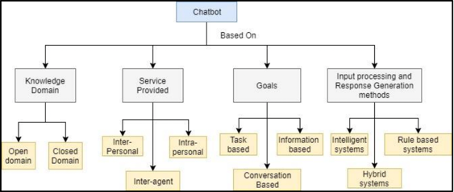
\includegraphics{F19_chatbotClassificatie.png}
    \captionsetup{justification=ce/brntering, singlelinecheck=false}    
    \caption{Classificaties en soorten van een chatbot.}
    \label{fig:chatbotTypes}
\end{figure}

Chatbots worden onderverdeeld in categorieën door gebruik te maken van enkele parameters. Voorbeelden van parameters zijn het kennisdomein, dienstverlening, de methode voor het verwerken van de input en het genereren van een antwoord en menselijke hulp en bouwmethode \autocite{Adamopoulou2020}. 

Twee grote categorieën waarin de soort chatbot verschillen zijn open domeinen en gesloten domeinen. Open domein chatbots vertellen ons meer over algemene onderwerpen die een zo goed mogelijk antwoord geven op de vraag van de gebruiker. Gesloten domein chatbots werken aan de hand van algemene domein kennis van de chatbot \autocite{Adamopoulou2020}. Nadelig hieraan is dat niet alle vragen even goed kunnen beantwoord worden \autocite{Kucherbaev2018}.

Een verdere onderscheid van chatbots zijn de soorten aangeboden diensten: ‘Interpersonal, ‘Intrapersonal en ‘Inter-agent’. Met een ‘Intrapersonal’ service communiceert hij de gekende informatie zoals openingsuren van een winkel, of trein boekingen met de eindgebruiker \autocite{Adamopoulou2020}. ‘Intrapersonal’ bots proberen de gebruiker te verstaan en te helpen zoals een echte mens. Deze gaan opzoek naar persoonlijke domein data van de gebruiker. Als laatste onderverdeling van dienstverlening bestaat de ‘Inter-agent’ chatbot. Deze bots communiceren met andere bots om hun informatie te delen. Op deze manier kunnen ze het best passende antwoorden schenken \autocite{Nimavat2017}.

De bots hebben altijd een specifiek doel. Daarvoor wordt er gekeken naar wat de chatbot wil bereiken. Wil de chatbot informatie verschaffen aan de gebruiker aan de hand van vaste middelen dan spreken we over informatieve chatbots. Bij het geval van ‘Task based’ zal de chatbot effectief een taak uitvoeren aan de hand van specifieke eisen. Als meest gebruikte vorm van chatbot is er de chat gebaseerde of conversatie chatbot. Deze is puur gericht om het juiste antwoord te verschaffen op de gestelde vraag (\autocite{Nimavat2017} \autocite{Adamopoulou2020}. 

De drie modellen die geklasseerd onder ‘respons en generation method’ stellen methodes voor die de vraagstelling in acht neemt en genereert een gepast antwoord. Als eerste bestaat er de ‘Rule based’ model. Deze bots worden zo getraind en geprogrammeerd om op specifieke zoektermen de juiste vooraf gedefinieerde antwoorden te verschaffen. De toepassing van \ac{FAQ} bot is hiervan een voorbeeld. Deze bot verschilt maar nauwelijks ten opzichte van een ‘Retrieval based model, wat meer flexibiliteit geeft. Het analyseert verschillende mogelijke bronnen aan de hand van ‘APIs’. Het laatste model is ‘Generative’.  Dit model is gebaseerd om op vorige berichten een antwoord te voorzien. Dit is het meest krachtigste model en het meest complexe om te programmeren en te trainen \autocite{Adamopoulou2020} \autocite{Hien2018}.

\subsection{Platformen om chatbots te bouwen}%
\label{sec:chatbotBouwen}



%%=============================================================================
%% Methodologie
%%=============================================================================

\chapter{\IfLanguageName{dutch}{Methodologie}{Methodology}}%
\label{ch:methodologie}

%% TODO: Hoe ben je te werk gegaan? Verdeel je onderzoek in grote fasen, en
%% licht in elke fase toe welke stappen je gevolgd hebt. Verantwoord waarom je
%% op deze manier te werk gegaan bent. Je moet kunnen aantonen dat je de best
%% mogelijke manier toegepast hebt om een antwoord te vinden op de
%% onderzoeksvraag.



%%=============================================================================
%% Proof-Of-Concept
%%=============================================================================


\chapter{Proof-Of-Concept}%
\label{ch:Proof-Of-Concept}


In dit hoofdstuk wordt omschreven op welke manier we onderzochte technologieën hebben toegepast op de probleemstelling van het bedrijf Lockit Rentals. De werking van eigen ontwikkelde toepassingen worden specifiek toegelicht op basis van gedocumenteerde informatie. Op vlak van de QR-codes is het doel om de huidige scan software te optimaliseren. Hierbij gaan er experimenten uitgevoerd worden om deze grondig te vergelijken. In het tweede deel zal de chatbot ontwikkeld worden aan de hand van het gekozen platvorm. Om aan te tonen dat nieuwe technieken een oplossing kunnen bieden, verwijs ik door naar de verwerkte resultaten \ref{ch:verwerkingresultaten}.

\section{Opbouw experimenten}%
\label{sec:toepassingenQR-coce scanners}

Zowel de nieuwe als de oude opstelling worden grondig getest in vier verschillende scenario’s. Daarnaast zijn er ook twee manieren om de toegangscode te bezitten. Allereerst kan de klant in het bezit zijn van een QR-code op papier. Alsook kunnen ze deze digitaal op de Lockit Rentals mobiele applicatie registreren. Beide manieren laat scan mogelijkheden toe. Dit zal een rol spelen in de aantal uitgevoerde experimenten waarbij constante variabelen van toepassing zijn. De QR-code dat gescand wordt door dezelfde testpersoon op hetzelfde apparaat zorgen voor betrouwbaar eindresultaat. 
Aangezien sommige omgevingsfactoren veranderen doorheen het proces zullen we ook de verlichtingssterkte meten uitgedrukt in lux. Deze waarde zal niet meegenomen worden bij de conclusie maar is gewoon ter illustratie. 
Op het einde van elke test wordt er een \ac{XLSX} bestand gecreëerd. Een voorbeeld hiervan is te zien op figuur \ref{fig:xlsxBestandExperiment}. Deze bestanden hebben steeds een logische naamgeving zodat we dit later kunnen verwerken in een duidelijke conclusie. In figuur x zien we de oplijsting van alle bestanden.


\begin{figure}
    \centering
    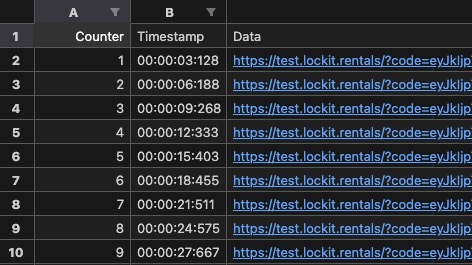
\includegraphics[width=0.8\textwidth]{graphics/F27_QR-data_uitlezing.jpg}
    \captionsetup{justification=centering, singlelinecheck=false}    
    \caption{Voorbeeld \ac{XLSX} bestand na uitvoeren van QR-code camera programma.}
    \label{fig:xlsxBestandExperiment}
\end{figure}}

\begin{figure}
    \centering
    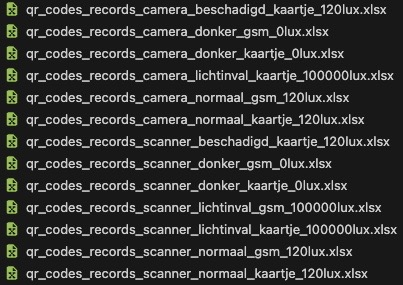
\includegraphics[width=0.8\textwidth]{graphics/F28_XLSX_opsomming.jpg}
    \captionsetup{justification=centering, singlelinecheck=false}    
    \caption{Opsomming alle \ac{XLSX} bestanden na uitvoeren van QR-code camera programma.}
    \label{fig:opsomming}
\end{figure}}


\section{Experiment 1: Huidige QR-camera}
\label{sec:huidigeToepassingScanners}

In het hoofdstuk \ref{sec:WerkingUnits} wordt aangetoond welk script er effectief actief is op de locker units. Na grondig onderzoek van de gebruikte camera’s kunnen we concluderen dat deze geen specifieke toestellen zijn om QR-codes te scannen. De camera op zich heeft veel configuratie en rekenkracht nodig om de QR-code waar te nemen en te kunnen capteren in bruikbare data. 

Om deze experimenten uit te voeren, ga ik gebruik maken van een eigen opstelling die de huidige scanner inclusief de software hanteert te zien op figuur \ref{fig:vooraanzichtUSBCamera} en \ref{fig:achteraanzichtUSBCamera}. Uiteraard maak ik enkele aanpassingen aan de code om ervoor te zorgen dat deze geschikt is voor de vergelijking.  Het is belangrijk om op te merken dat deze wijzigingen geen invloed zullen hebben op de eindresultaten van de experimenten. Deze aangepaste code wordt weergegeven in listing \ref{lst:huidigeQR-codeData}.

\begin{figure}[h]
    \centering
    \begin{minipage}{0.45\textwidth}
        \centering
        \rotatebox{-90}{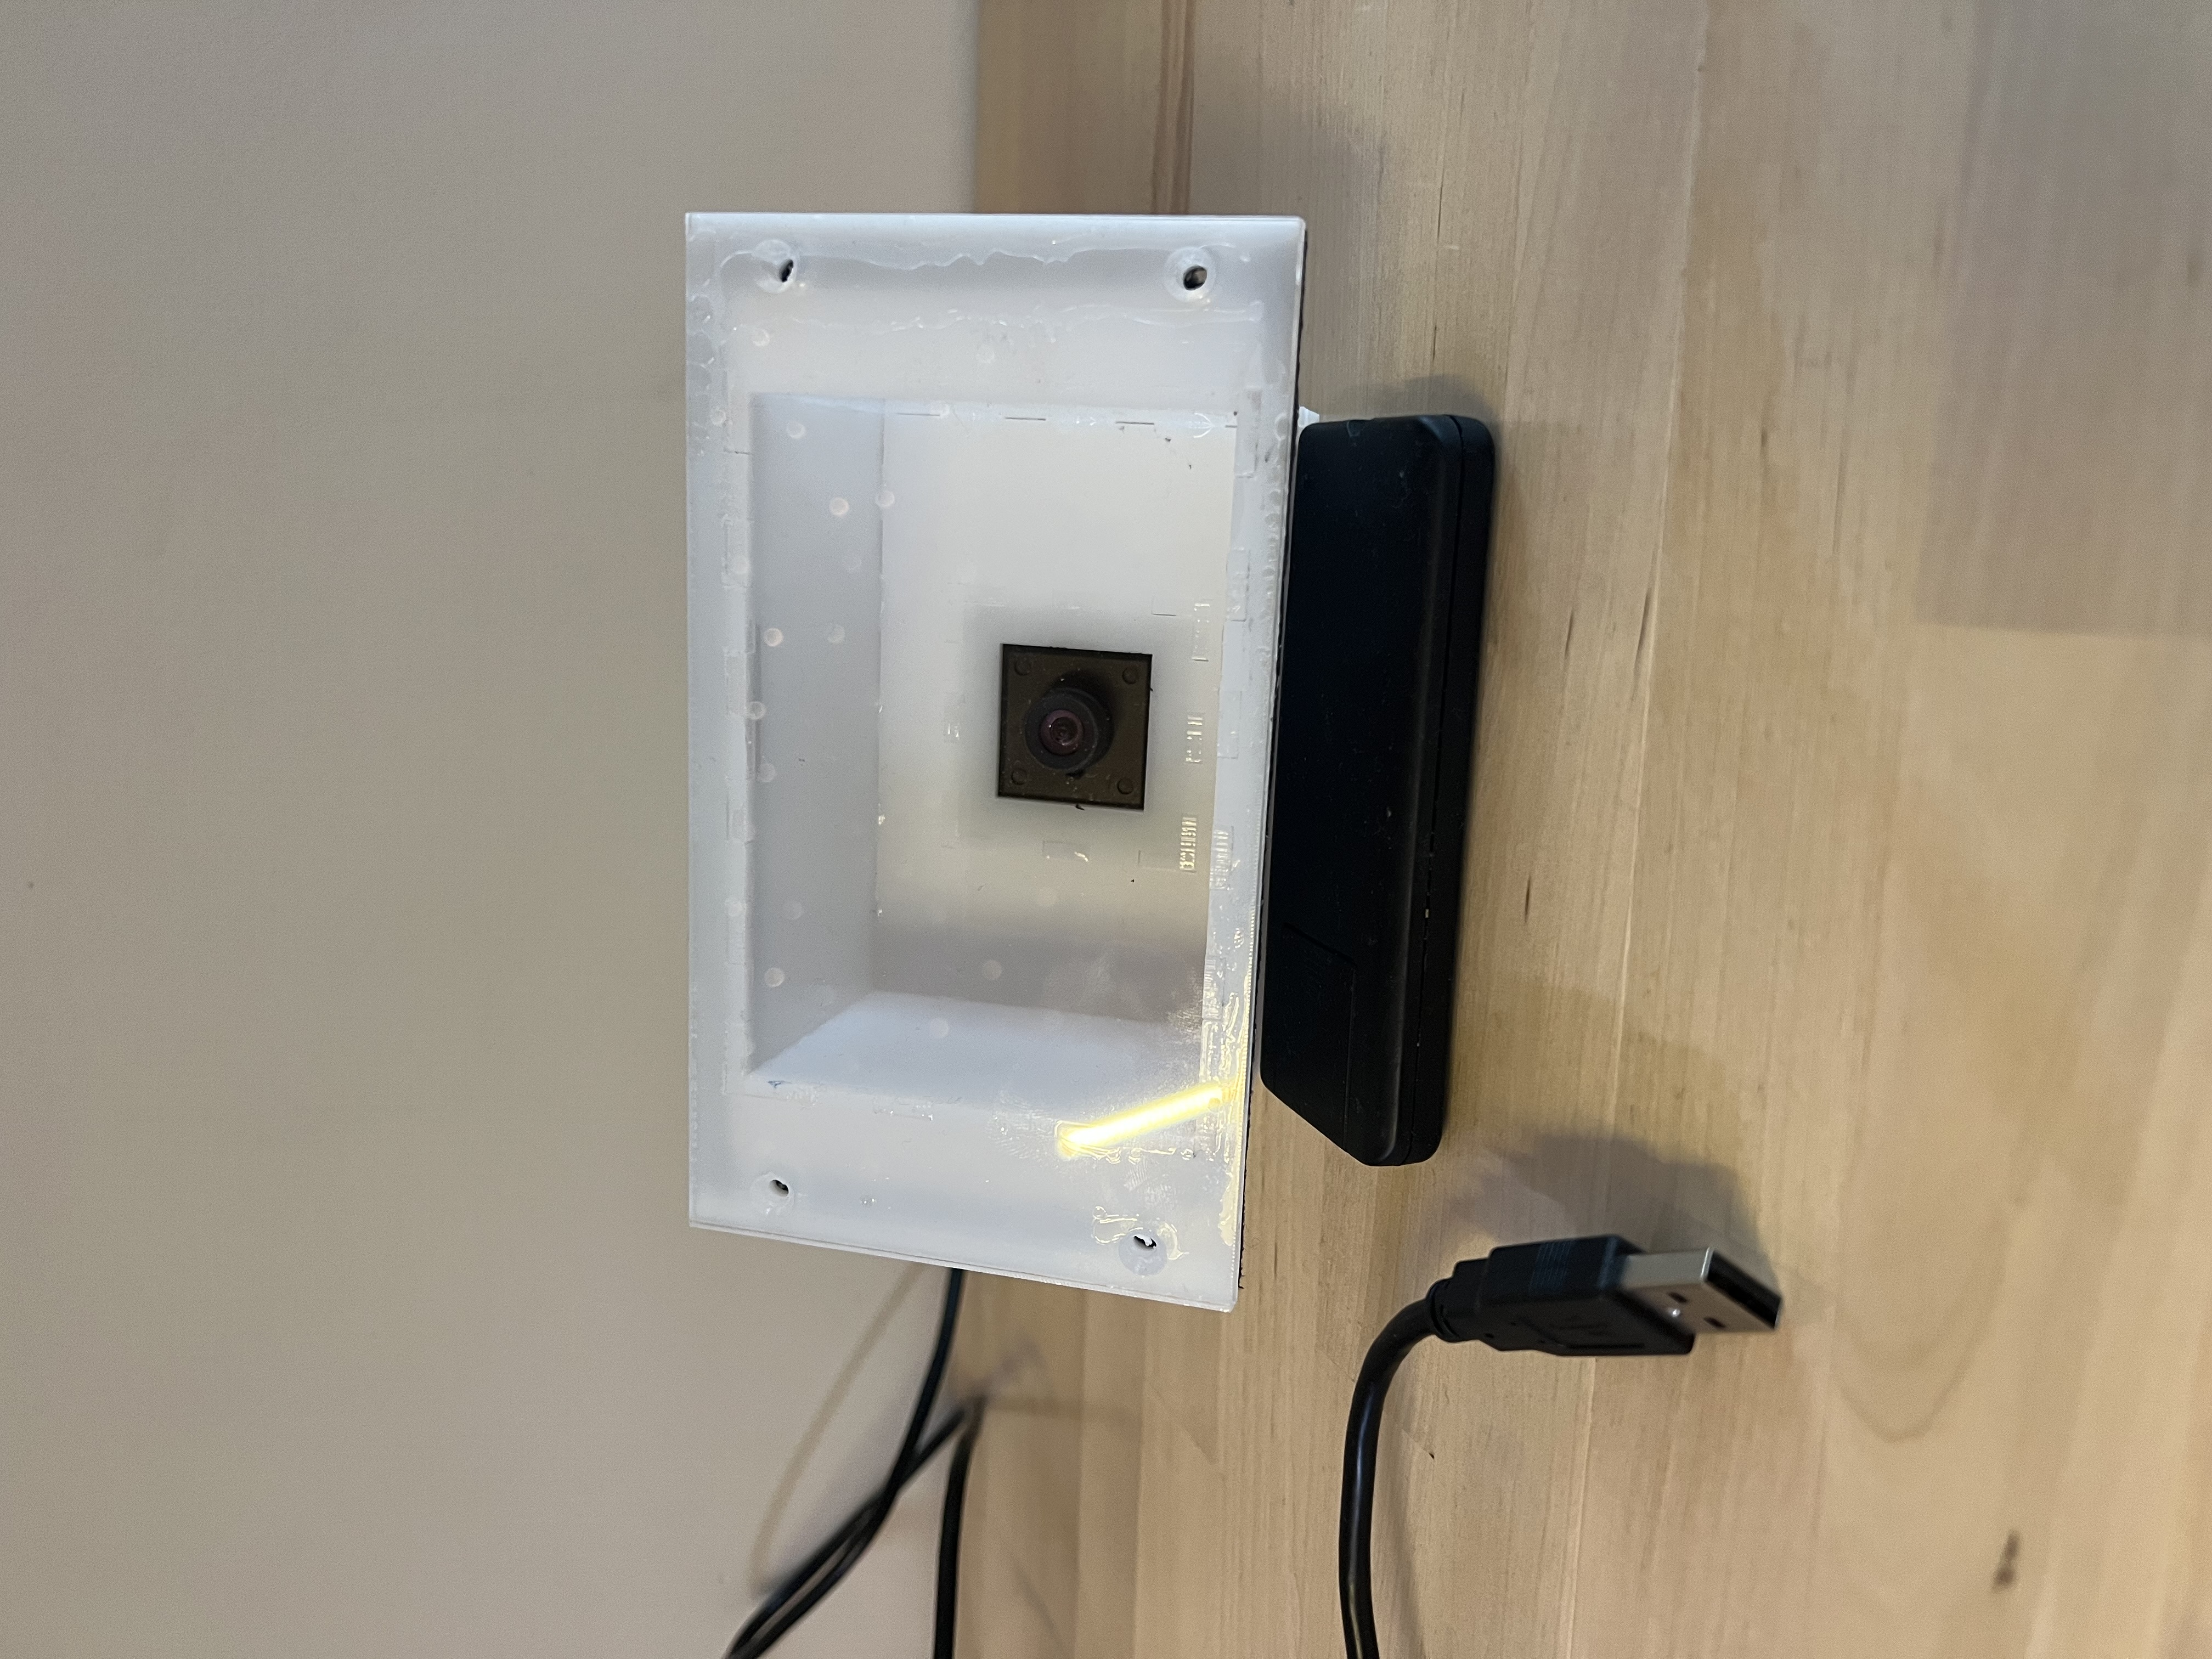
\includegraphics[width=\textwidth]{graphics/F22_USBCamera_front.jpeg}}
        \caption{Vooraanzicht USB QR-camera}
        \label{fig:vooraanzichtUSBCamera}
    \end{minipage}
    \hfill
    \begin{minipage}{0.45\textwidth}
        \centering
        \rotatebox{-90}{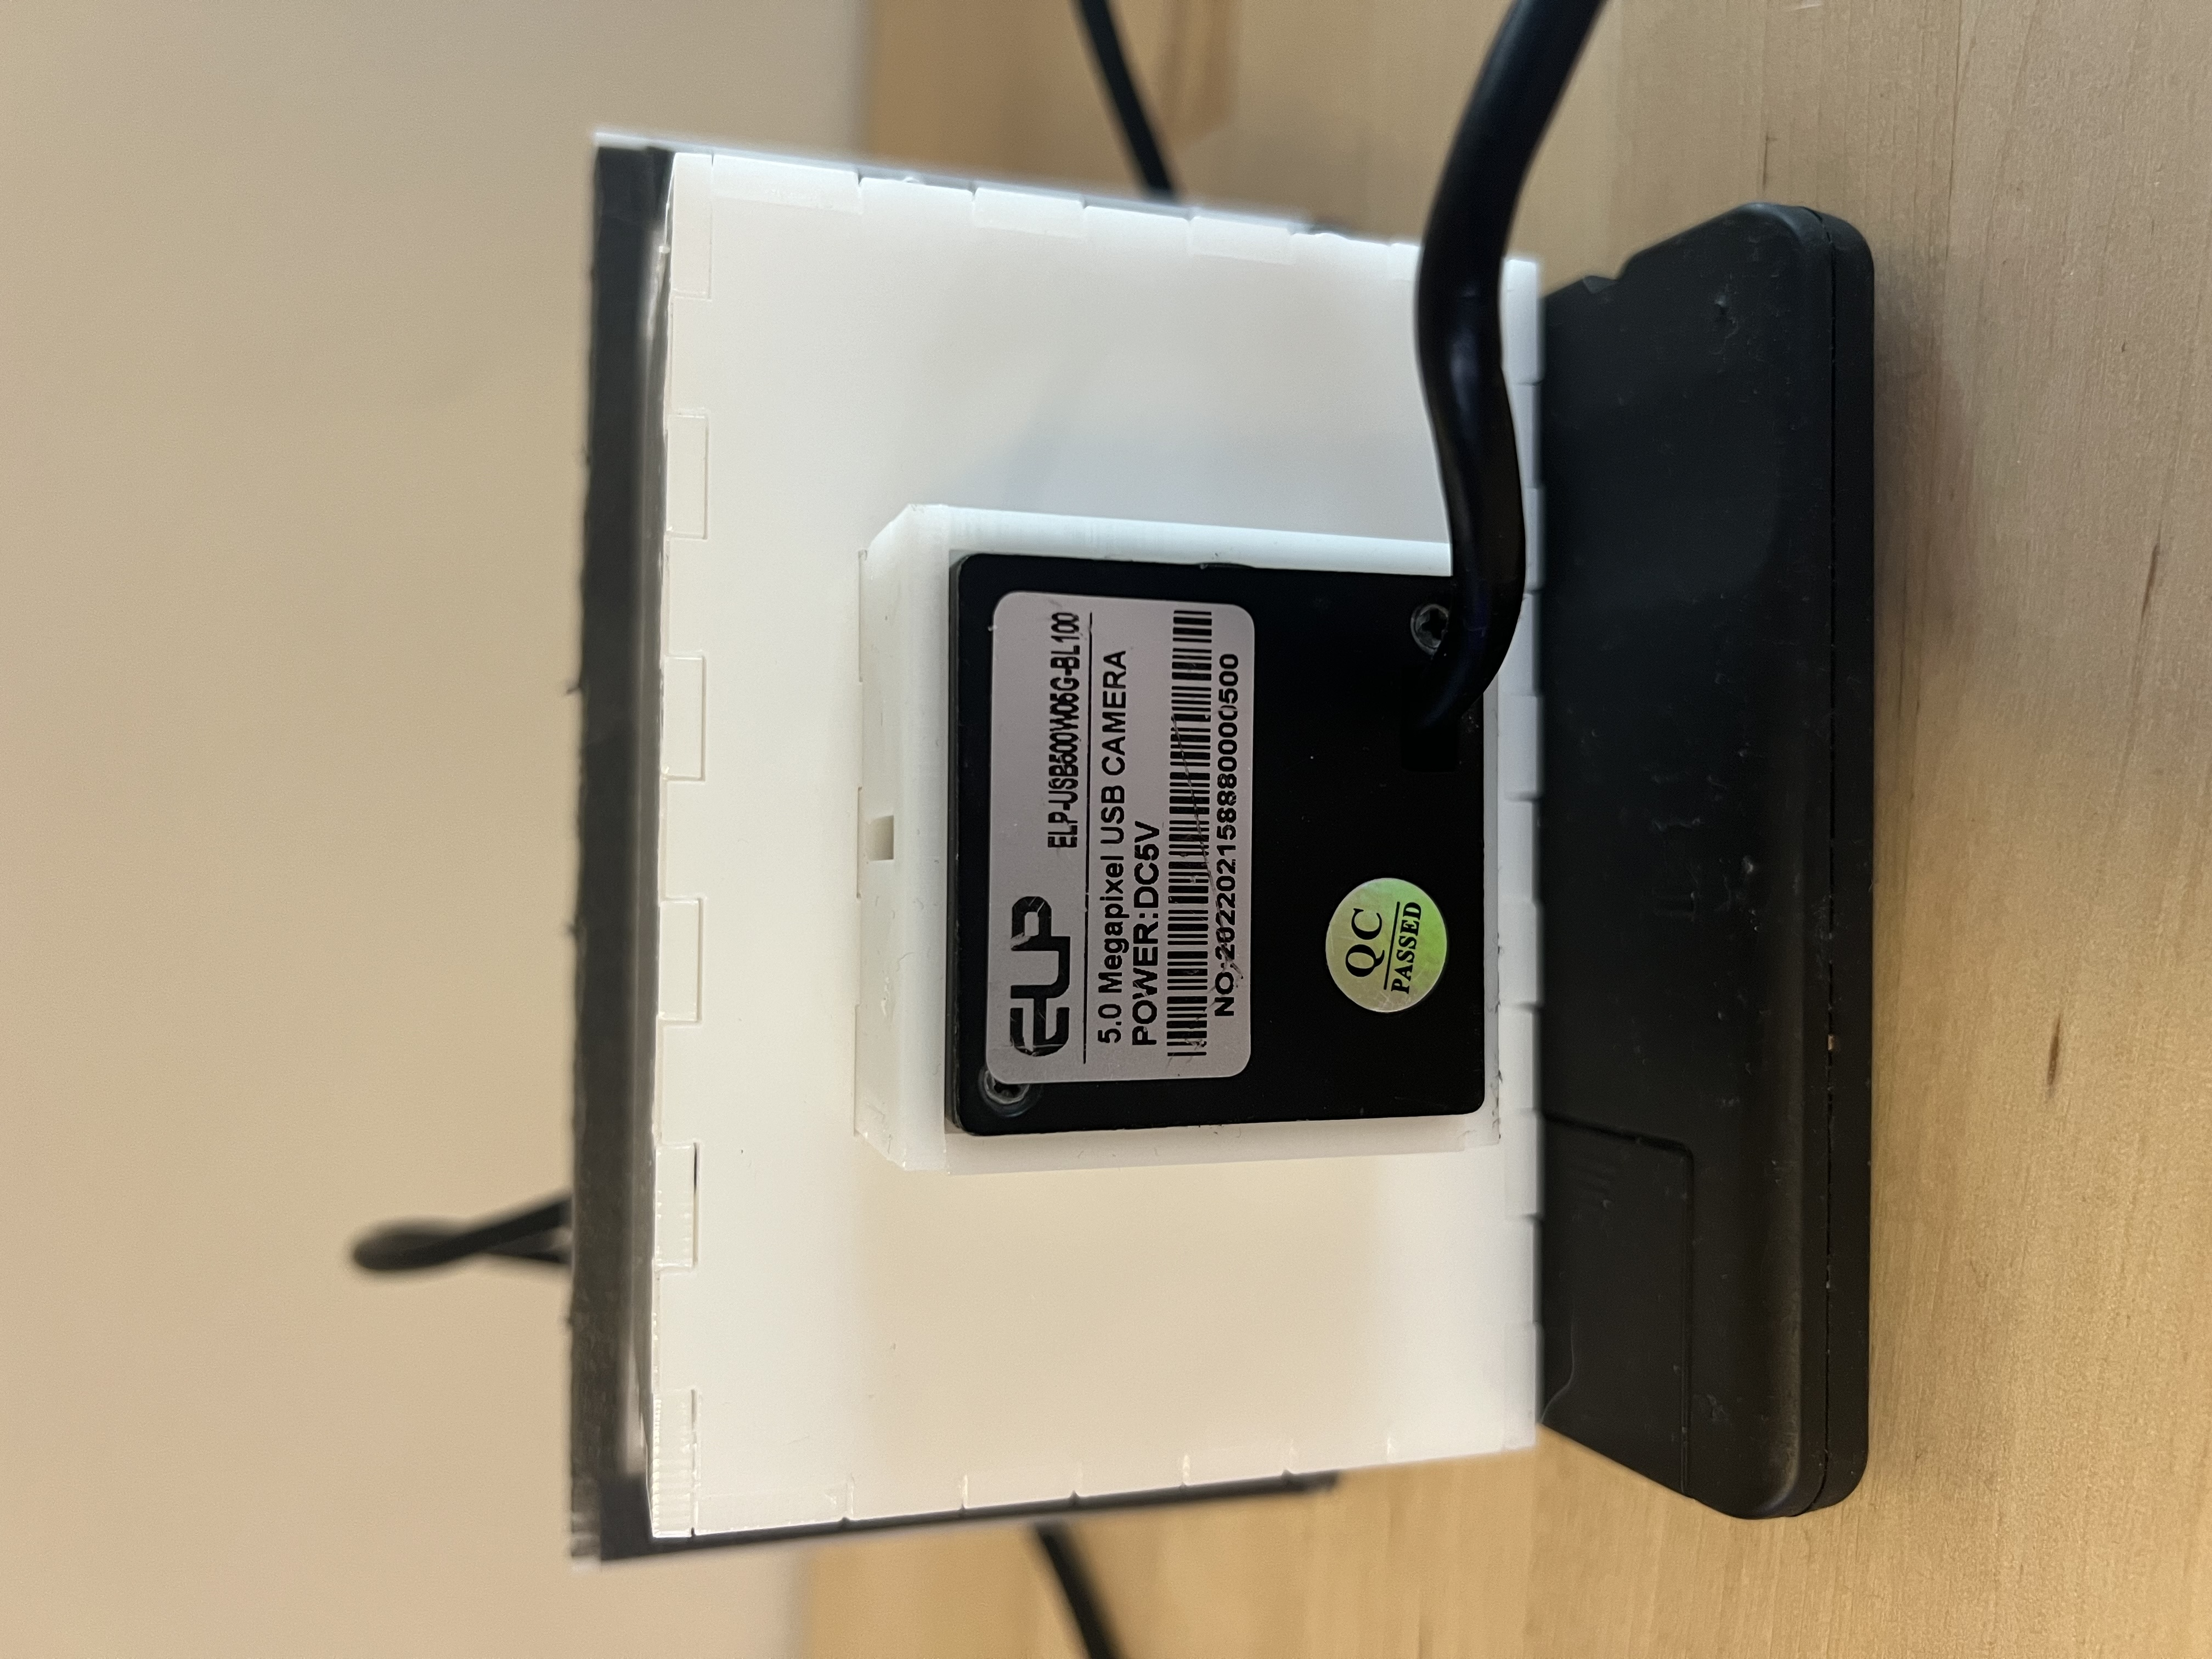
\includegraphics[width=\textwidth]{graphics/F23_USBCamera_back.jpeg}}
        \caption{Achteraanzicht USB QR-camera}
        \label{fig:achteraanzichtUSBCamera}
    \end{minipage}
\end{figure}


\begin{lstlisting}[language=Python, caption={Python script voor experiment van QR-code camera.}, label=lst:huidigeQR-codeData, numbers=left]
    import cv2  # Importeer de cv2-bibliotheek voor het werken met beeldverwerking
    import time  # Importeer de time-bibliotheek om pauzes in de uitvoering van het programma te creëren
    import pyzbar.pyzbar as pyzbar  # Importeer de pyzbar-bibliotheek voor het decoderen van QR-codes
    from datetime import datetime  # Importeer de datetime-bibliotheek om tijdstempels te maken
    from openpyxl import Workbook  # Importeer de openpyxl-bibliotheek voor het werken met Excel-bestanden
    
    camera = cv2.VideoCapture(0)  # Gebruik de cv2-bibliotheek om toegang te krijgen tot de camera
    counter = 1  # Initialiseer een teller om bij te houden hoeveel QR-codes zijn gescand
    start_time = datetime.now()
    
    # Maak een nieuw werkboek / excel aan en selecteer het actieve werkblad
    workbook = Workbook()
    worksheet = workbook.active
    # Stel de kolomkoppen in voor het Excel-bestand
    worksheet['A1'] = 'Counter'
    worksheet['B1'] = 'Timestamp'
    worksheet['C1'] = 'Data'
    
    def decode_qr(image):  # Functie om QR-codes te decoderen
        try:
            gray = cv2.cvtColor(image, cv2.COLOR_BGR2GRAY)  # Zet het kleurenbeeld om in grijswaarden
            barcodes = pyzbar.decode(gray, symbols=[pyzbar.ZBarSymbol.QRCODE])  # Decodeer QR-codes
            if barcodes:
                timestamp = (datetime.now() - start_time).total_seconds()  # Bereken het tijdsverschil vanaf het begin
                timestamp_formatted = time.strftime('%H:%M:%S:%f', time.gmtime(timestamp))  # Maak de tijdstempel
                return (barcodes[0].data.decode(), timestamp_formatted)  # Return de gedecodeerde gegevens en tijdstempel
        except Exception as e:
            print(e)
        return None
    
    while counter <= 50:
    ret, frame = camera.read() # Lees de afbeelding van de camera
    
        if not ret:
            break
        qr_data = decode_qr(frame) # Decodeer QR-code in afbeelding
        if qr_data:
            timestamp = (datetime.now() - start_time).total_seconds() * 1000 # Formatteer de timestamp
            hours, remainder = divmod(int(timestamp), 3600000)
            minutes, remainder = divmod(remainder, 60000)
            seconds, milliseconds = divmod(remainder, 1000)
            timestamp_formatted = f"{hours:02}:{minutes:02}:{seconds:02}:{milliseconds:03}"
            # Print de QR-code informatie en voeg het toe aan de Excel-sheet
            print(f'{counter} | Timestamp: {timestamp_formatted} | Data: {qr_data[0]}')
            # Normaal doen we hier het POST request naar de server zie originele code
            row = (counter, timestamp_formatted, qr_data[0])
            worksheet.append(row)
            counter += 1
        time.sleep(3) # Wacht 3 seconden tussen elke frame
    
    
    end_time = datetime.now()
    
    # Sla het Excel bestand op
    workbook.save('qr_codes_records_camera_normaal_gsm_120lux.xlsx')
    
    print(f"Counter reached {counter - 1}. Exiting program. Final time of scanning: {end_time - start_time}")
    camera.release() # Beëindig het gebruik van de camera    
\end{lstlisting}

\subsection{Resultaten huidig QR-camera experiment}
\label{sec:huidigeToepassingScannersExperiment}

Hieronder bevinden zich de tabellen met daarin de eindresultaten van het experiment met de huidige QR-camera. Er zijn telkens 50 QR-codes gescand met uitzondering van QR-codes in de beschadigde situatie.

\begin{table}[h]
    \centering
    \begin{tabular}{ c|c|c|c }
        \cline{2-4}
        & \textbf{\textit{QR-code op papier}} & \textbf{\textit{QR-code op gsm}} & \textbf{\textit{Verlichtingssterkte}} \\
        \cline{2-4}        
        \hline
        \textbf{\textit{1. Normaal}} &  230,402 s & 189,09 s & 120 lux \\
        \hline
        \textbf{\textit{2. Lichtinval}} & 204,729 s & 275,128 s & 100.000 lux \\
        \hline
        \textbf{\textit{3. Donker}} & 517,394 s & 166,856 s & 5 lux \\
        \hline        
    \end{tabular}
    \captionsetup{justification=centering}
    \caption{De waarden in de tabel zijn uitgedrukt in milliseconden (ms). Geef de resultaten weer van de huidige QR-camera experiment.}
    \label{tab:3expeQR-camera}
\end{table}

Het experiment dat beschadigde QR-codes omvat zal doorgaan met een set van acht QR-codes die beschadigd of onleesbaar gemaakt zijn. Deze QR-codes zijn zichtbaar op figuur \ref{fig:beschadigdeQR-codes} en zijn gerangschikt op basis van toenemende mate van beschadiging.

\begin{table}[h]
    \centering
    \begin{tabular}{ c|c }
        \cline{2-2}
        & \textbf{\textit{Beschadigd}} \
        \cline{2-2}
        \textbf{\textit{QR-code 1}} & 3,178 s \
        \cline{2-2}
        \textbf{\textit{QR-code 2}} & 15,588 s \
        \cline{2-2}
        \textbf{\textit{QR-code 3}} & 21,788 s \
        \cline{2-2}
        \textbf{\textit{QR-code 4}} & 99,403 s \
        \cline{2-2}
        \textbf{\textit{QR-code 5}} & / \
        \cline{2-2}
        \textbf{\textit{QR-code 6}} & / \
        \cline{2-2}
        \textbf{\textit{QR-code 7}} & / \
        \cline{2-2}
        \textbf{\textit{QR-code 8}} & 158,377 s \
        \cline{2-2}
    \end{tabular}
    \captionsetup{justification=centering}
    \caption{De waarden in de tabel zijn uitgedrukt in seconden (s). De verlichtingssterkte bij deze uitwerking is 120lux. De QR-codes in kwestie zijn te vinden in figuur \ref{fig:beschadigdeQR-codes}.}
    \label{tab:omgezette_tabel_seconds}
\end{table}

\begin{figure}
    \centering
    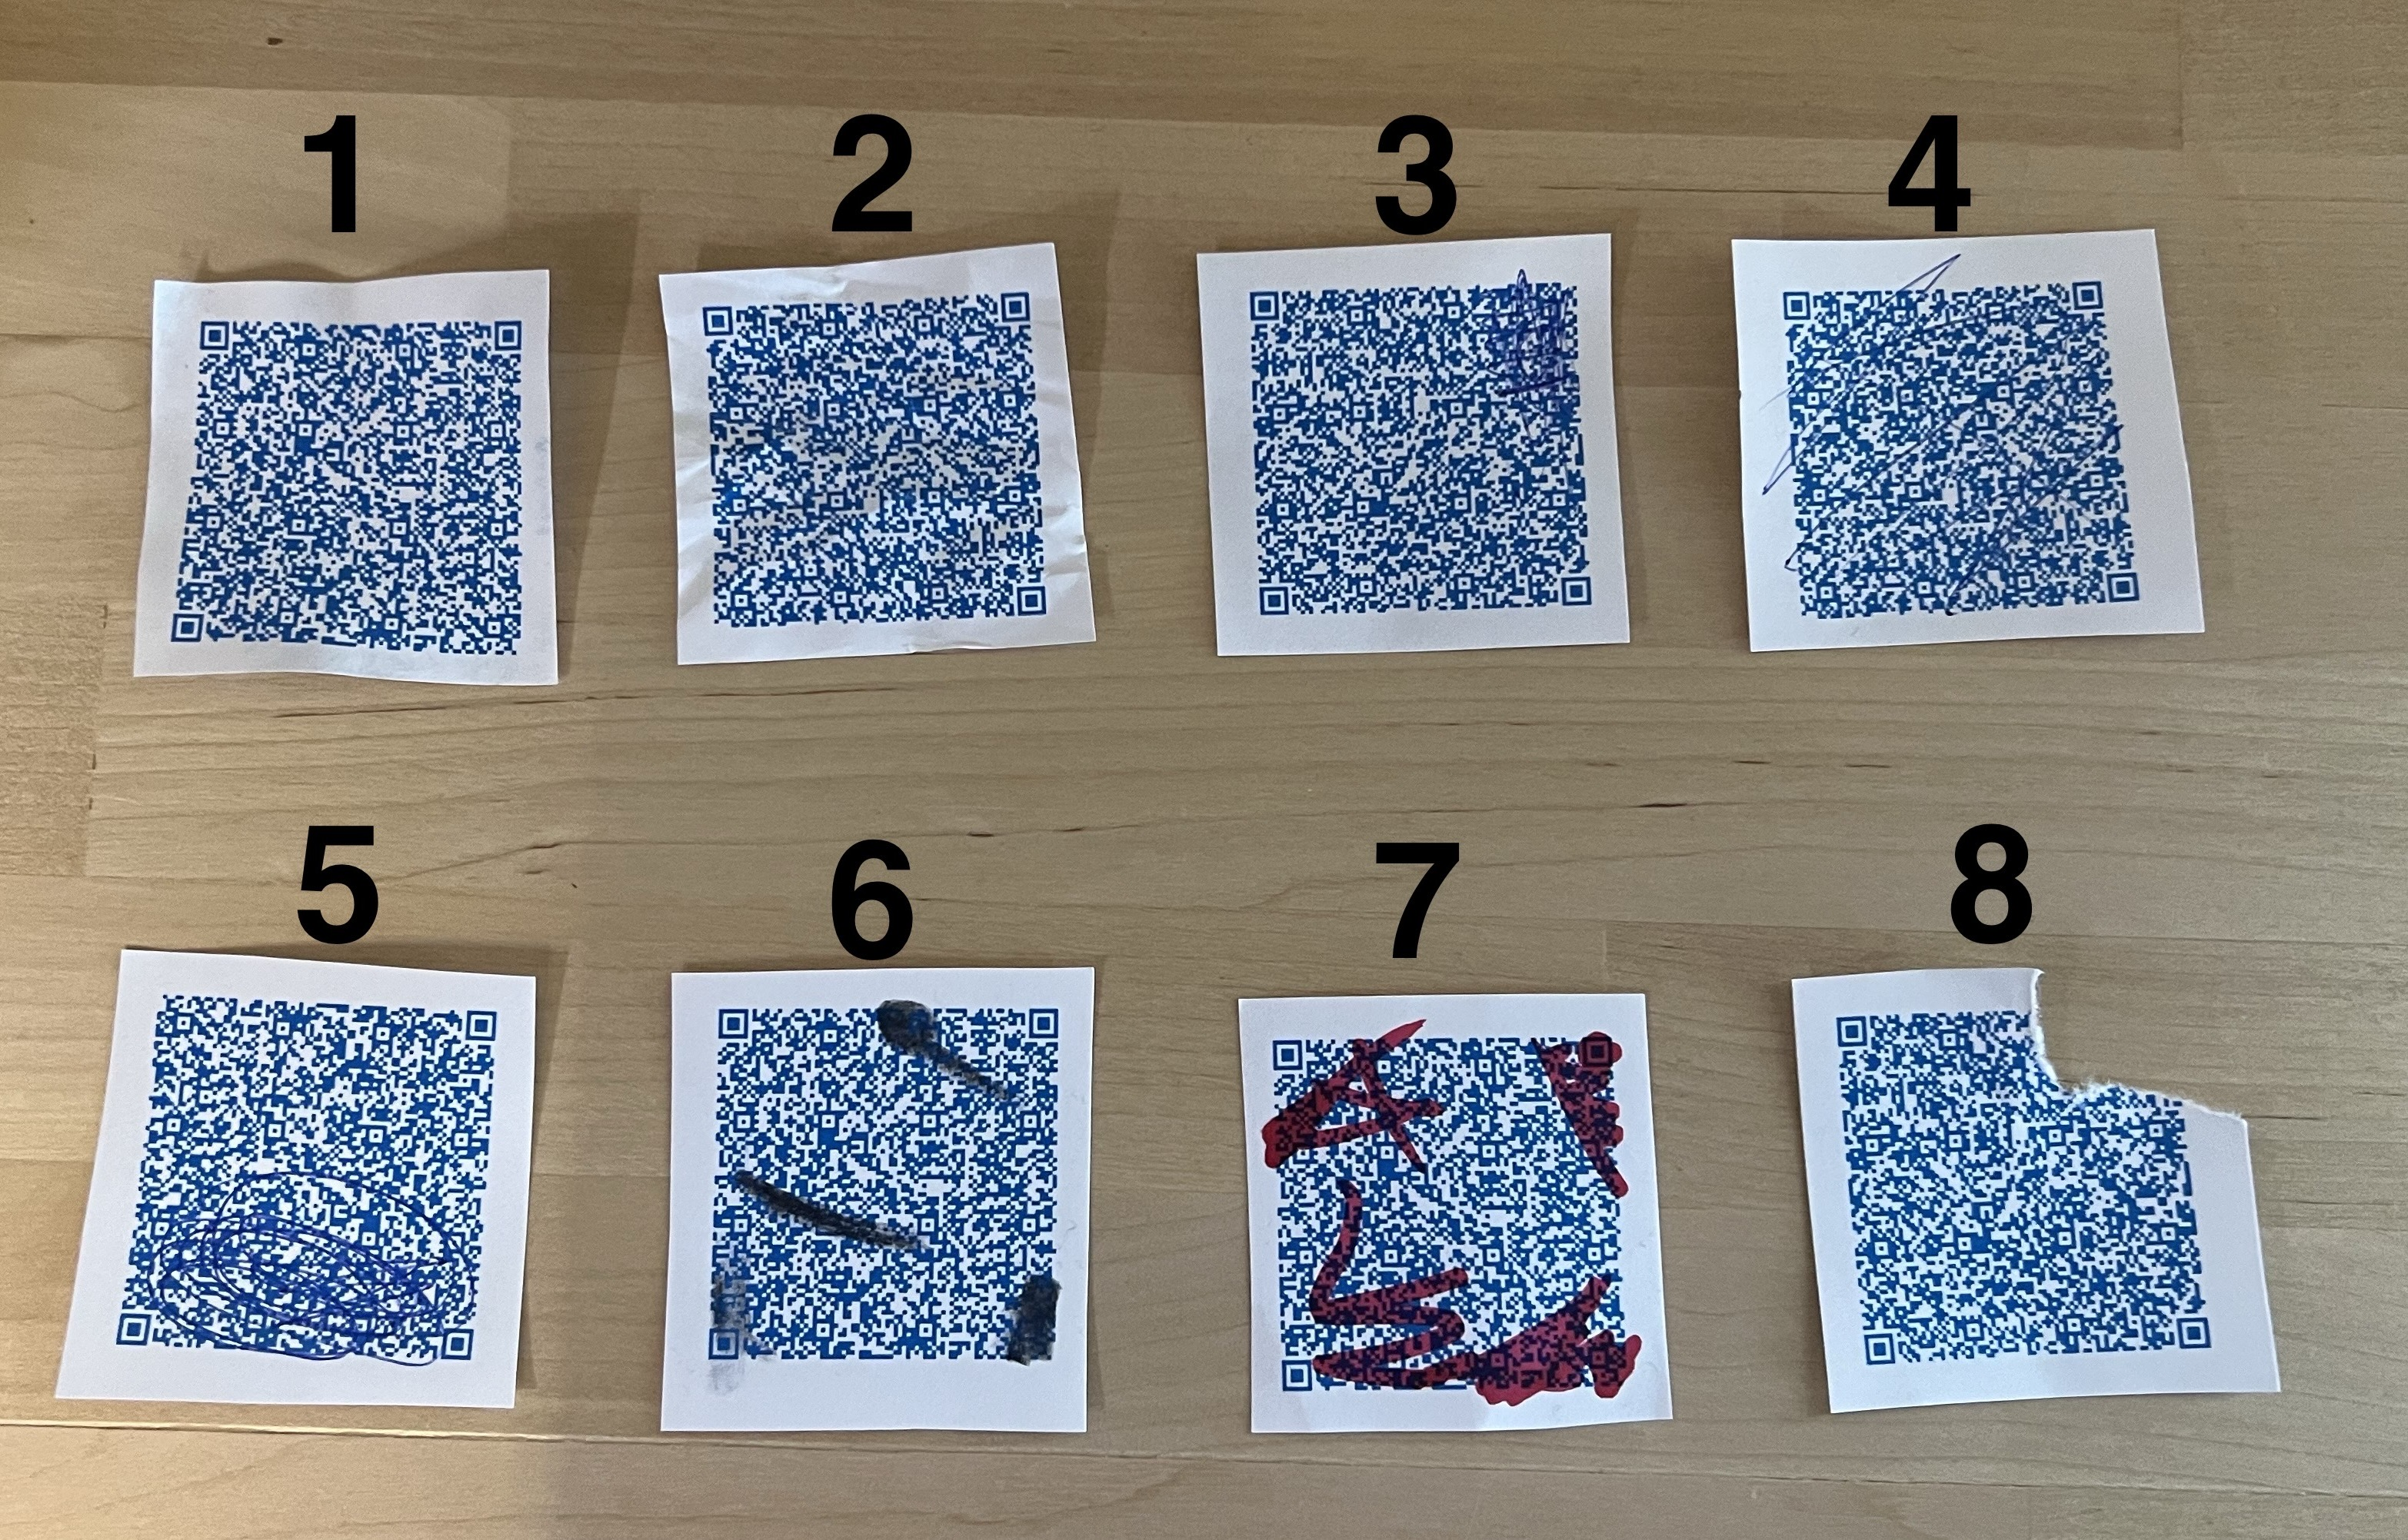
\includegraphics[width=0.8\textwidth]{graphics/F33_setBeschadigdeQR-codes.jpeg}
    \captionsetup{justification=centering, singlelinecheck=false}    
    \caption{Set van acht beschadigde QR-codes gerangschikt op basis van toenemende mate van beschadiging.}
    \label{fig:beschadigdeQR-codes}
\end{figure}}

\section{Experiment 2: Uitwerking nieuwe QR-scanner}
\label{sec:nieuweToepassing}

Wat opvalt bij het herschrijven en aanpassen van de bestaande scanner software is dat deze camera heel veel configuratie nodig heeft. We moeten de camera gaan initialiseren. Daarna moet de camera voortdurend de frames opnemen en bekijken of er een QR-code in beeld gekomen is. Dit proces neemt echter veel middelen in beslag waardoor de Raspberry PI oververhit kan worden zeker bij langdurige operaties in warme omgevingen.

Als we kijken naar hedendaagse scanners zoals kassasystemen en toegangscontrolesystemen bevatten deze vaste gespecialiseerde QR-code scanners. Na onderzoek heb ik een QR-code scanner gevonden en aangekocht die gespecialiseerd is om zowel ééndimensionale als tweedimensionale barcodes uit te lezen. De aangekochte scanner is afgebeeld op figuur \ref{fig:scannerBack}, \ref{fig:scannerFront} en \ref{fig:scannerSide}. In figuur \ref{fig:handleidingNieuweQRScanner} bevinden zich alle technische specificaties van de aangekochte QR-scanner. Bij de aankoop van deze QR-code scanner is er een handleiding met daarin alle mogelijke configuraties. Deze zijn zeer divers en kunnen een positieve invloed hebben op het scannen van QR-codes. Hieronder volgt een lijst met een aantal belangrijke configuratiemogelijkheden van dit toestel.

\begin{itemize}
    \item Het instellen van de USB virtuele poort, hierdoor kan de computer de USB poort herkennen en initialiseren. 
    \item De vertraging instellen als we éénzelfde QR-code na elkaar proberen te scannen. Deze is op het gebruikte toestel ingesteld op 3000 milliseconden. (TODO verwijzing figuur)
    \item Het toestel is geconfigureerd opdat er geen periode verstrijkt waarin we geen module kunnen lezen na het inlezen van een eerder gescande QR-code. (TODO verwijzing figuur)
    \item De lichten kunnen aan -of uitgezet worden.
    \item Een piepsignaal kan aan -of uitgezet worden wanneer de QR-code succesvol is uitgelezen.
    \item ...
\end{itemize}



\begin{figure}[h]
    \centering
    \begin{minipage}{0.32\textwidth}
        \centering
        \rotatebox{-90}{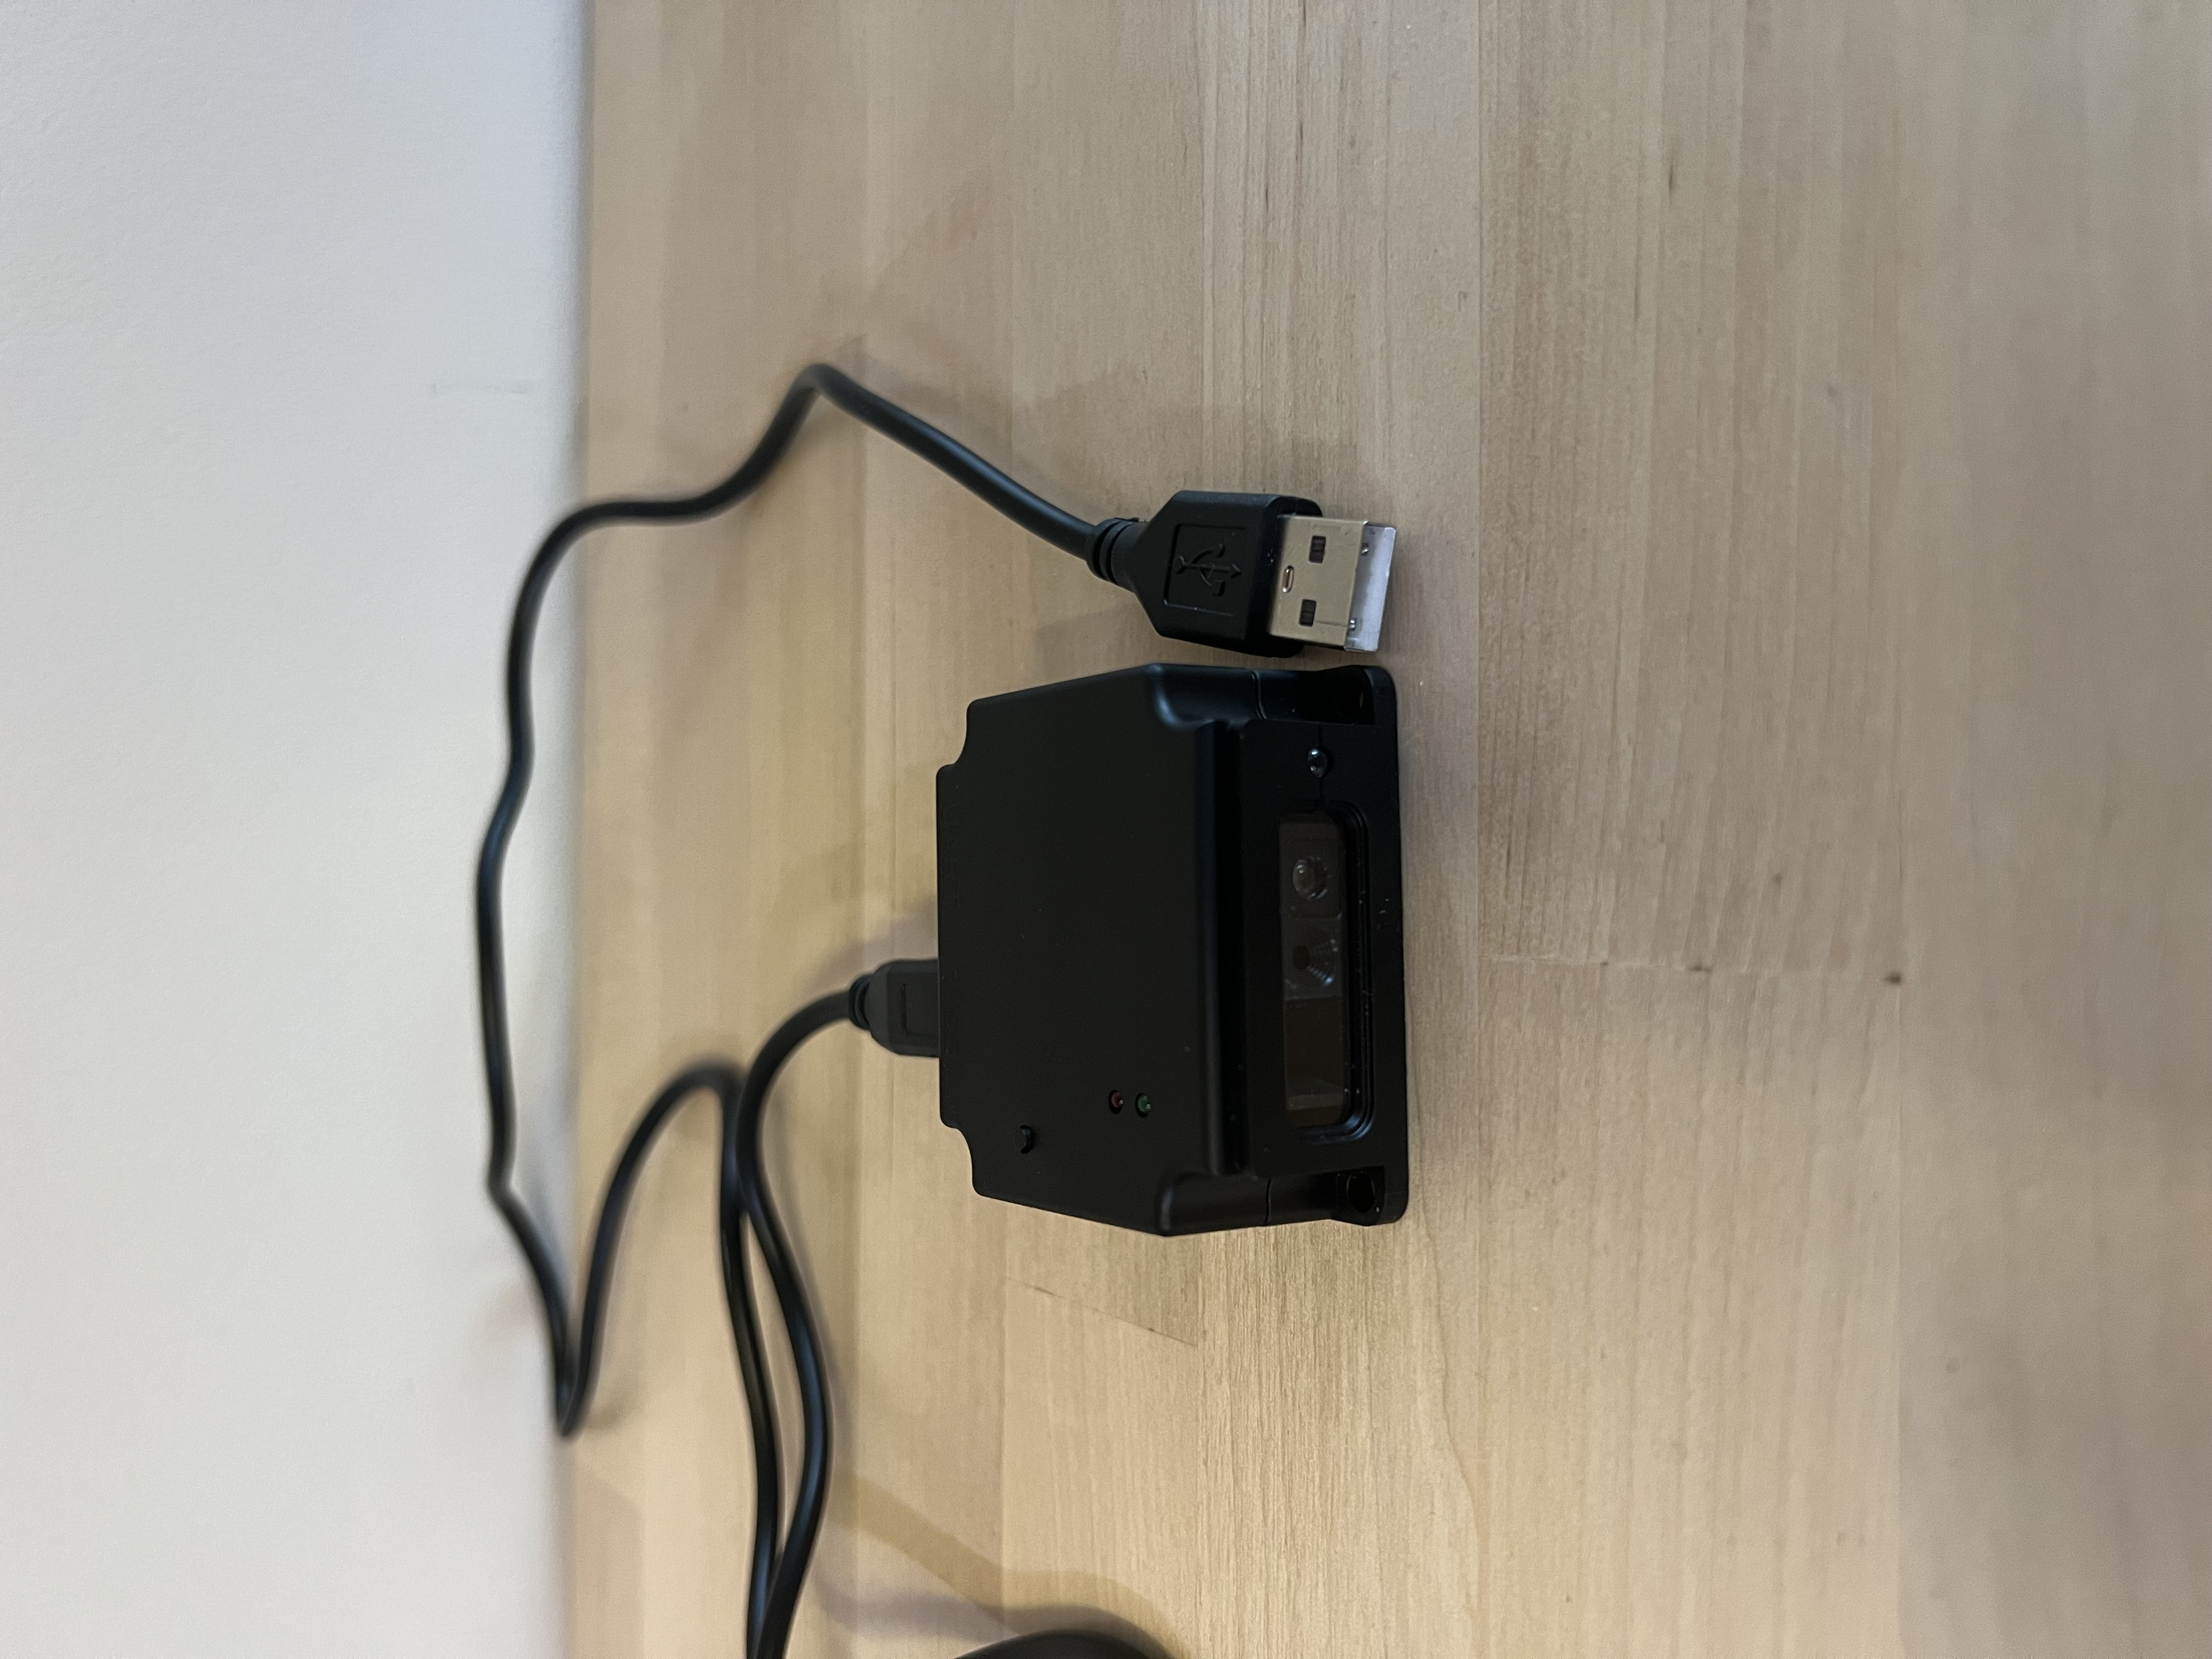
\includegraphics[width=\textwidth]{graphics/F24_scanner_back.jpeg}}
        \caption{Achterkant QR-scanner}
        \label{fig:scannerBack}
    \end{minipage}
    \hfill
    \begin{minipage}{0.32\textwidth}
        \centering
        \rotatebox{-90}{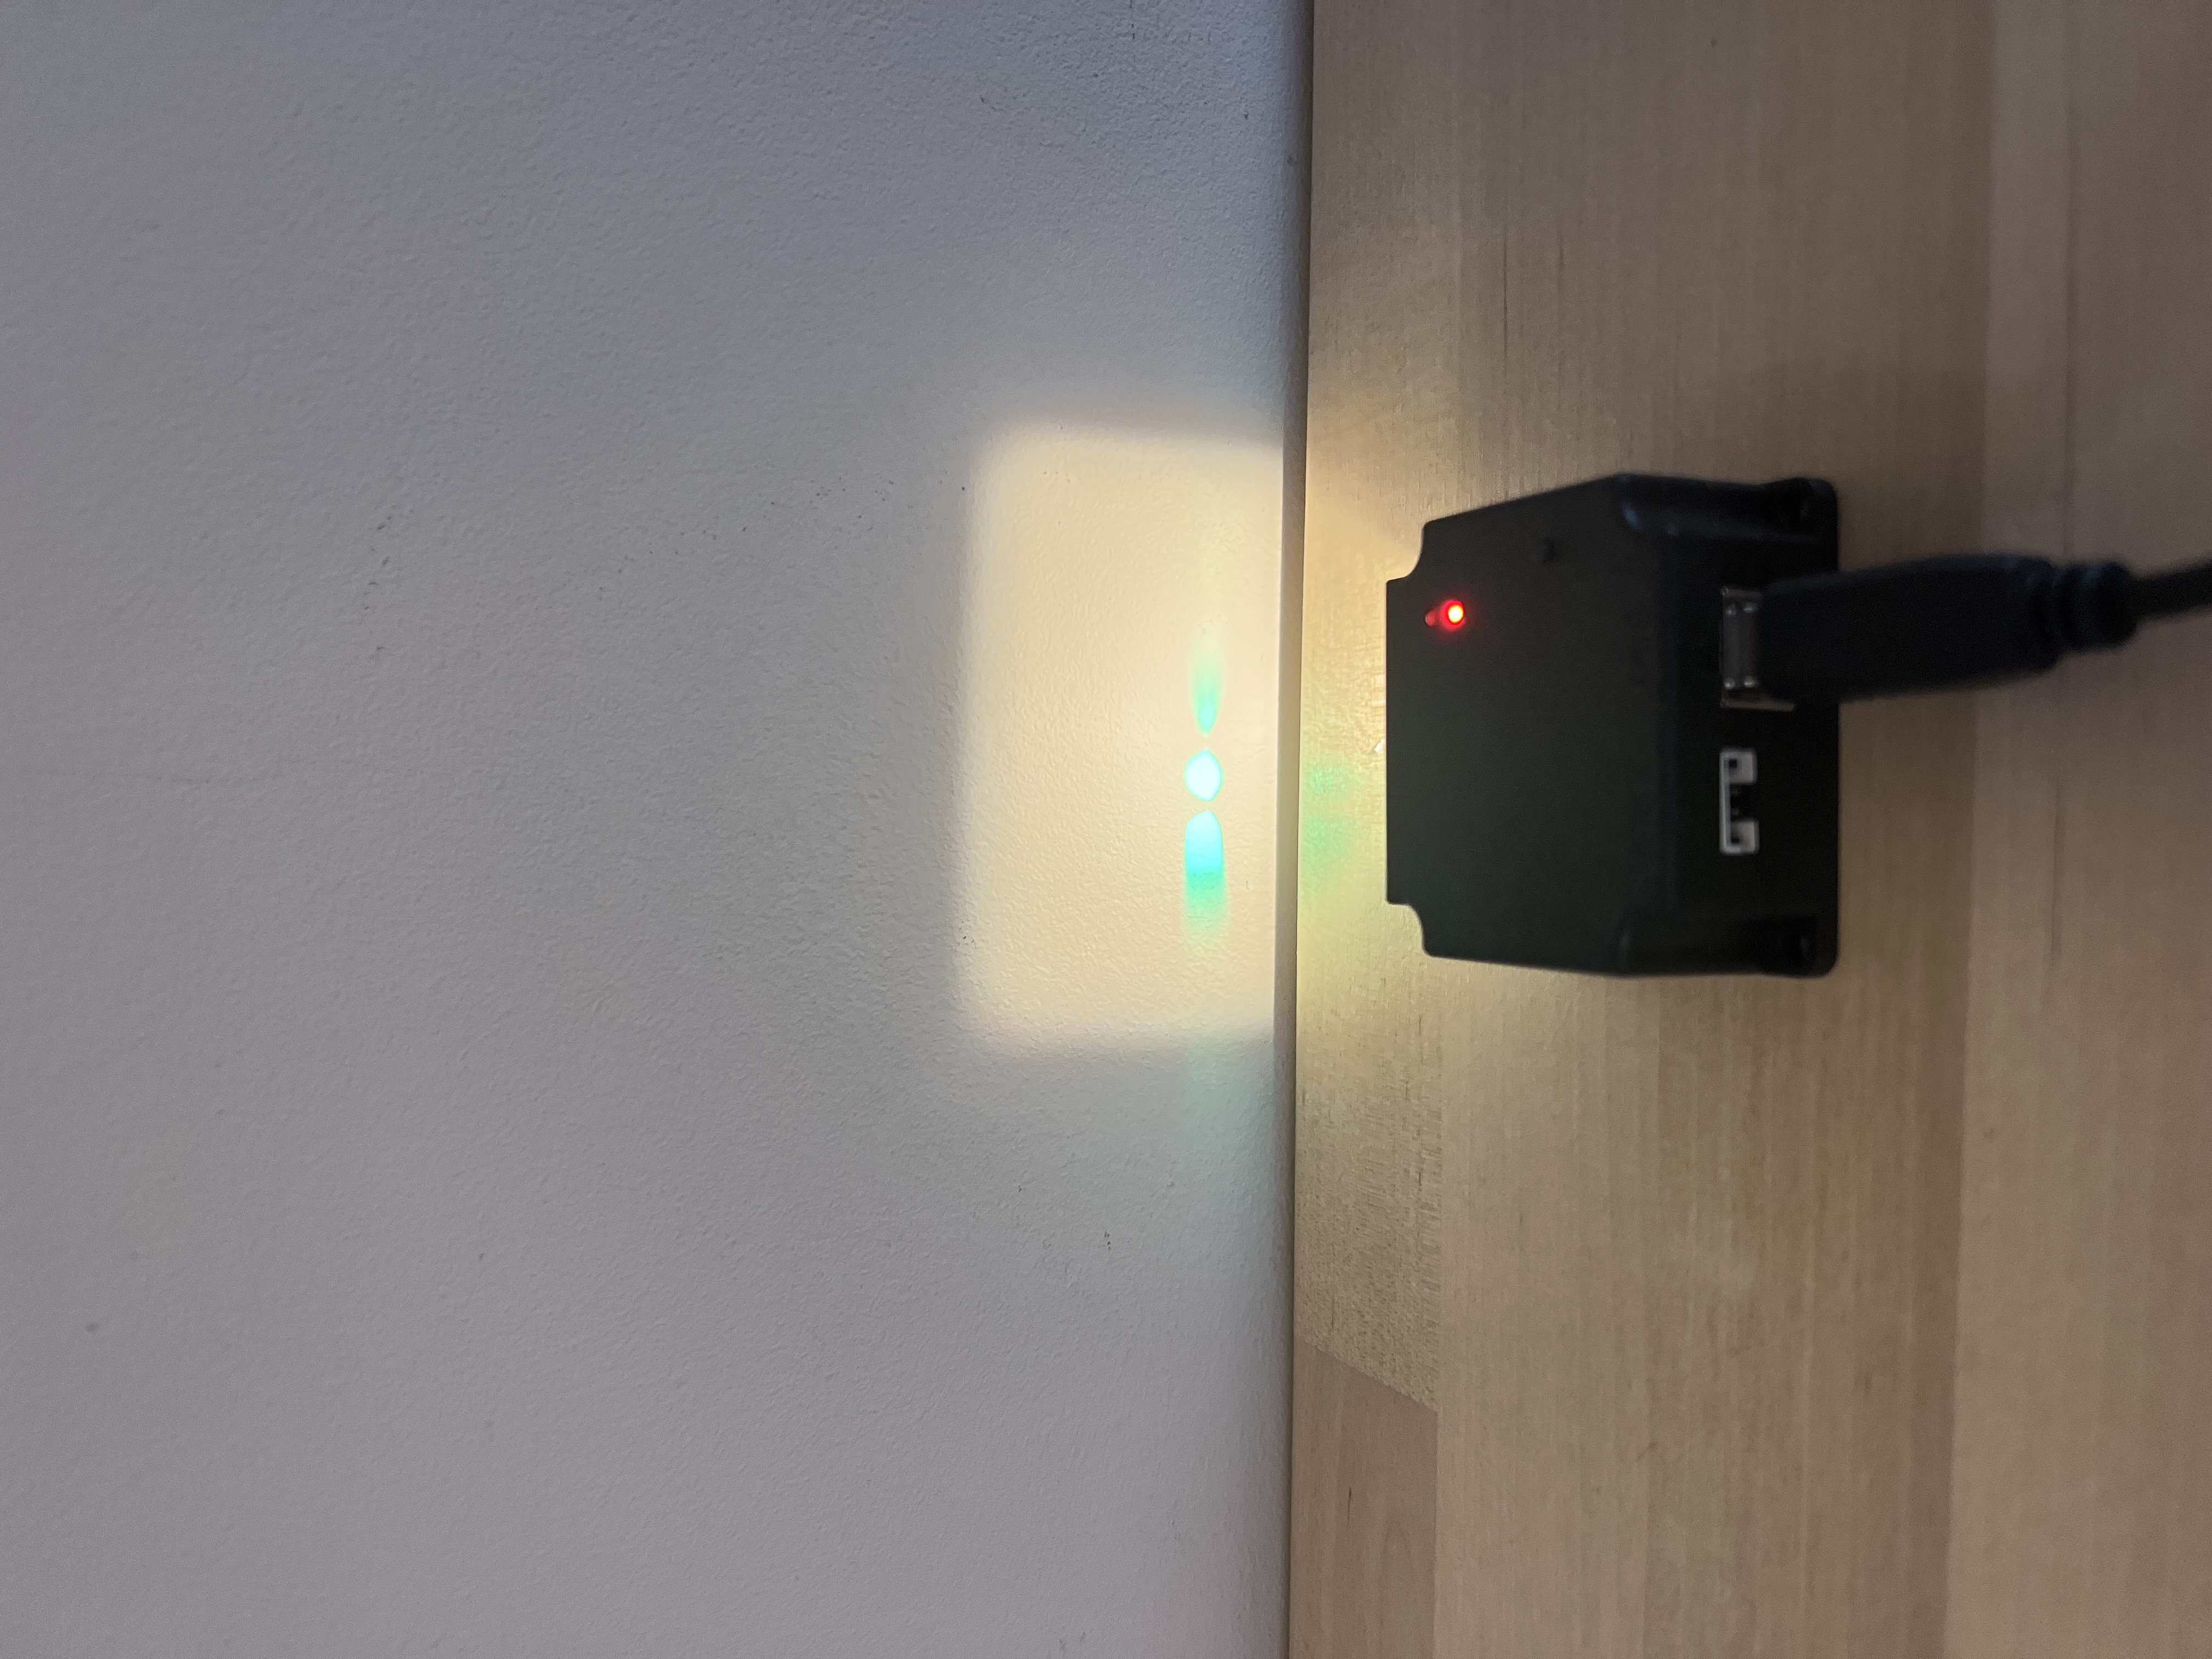
\includegraphics[width=\textwidth]{graphics/F25_scanner_front.jpeg}}
        \caption{Vooraanzicht QR-scanner}
        \label{fig:scannerFront}
    \end{minipage}
    \begin{minipage}{0.32\textwidth}
        \centering
        \rotatebox{-90}{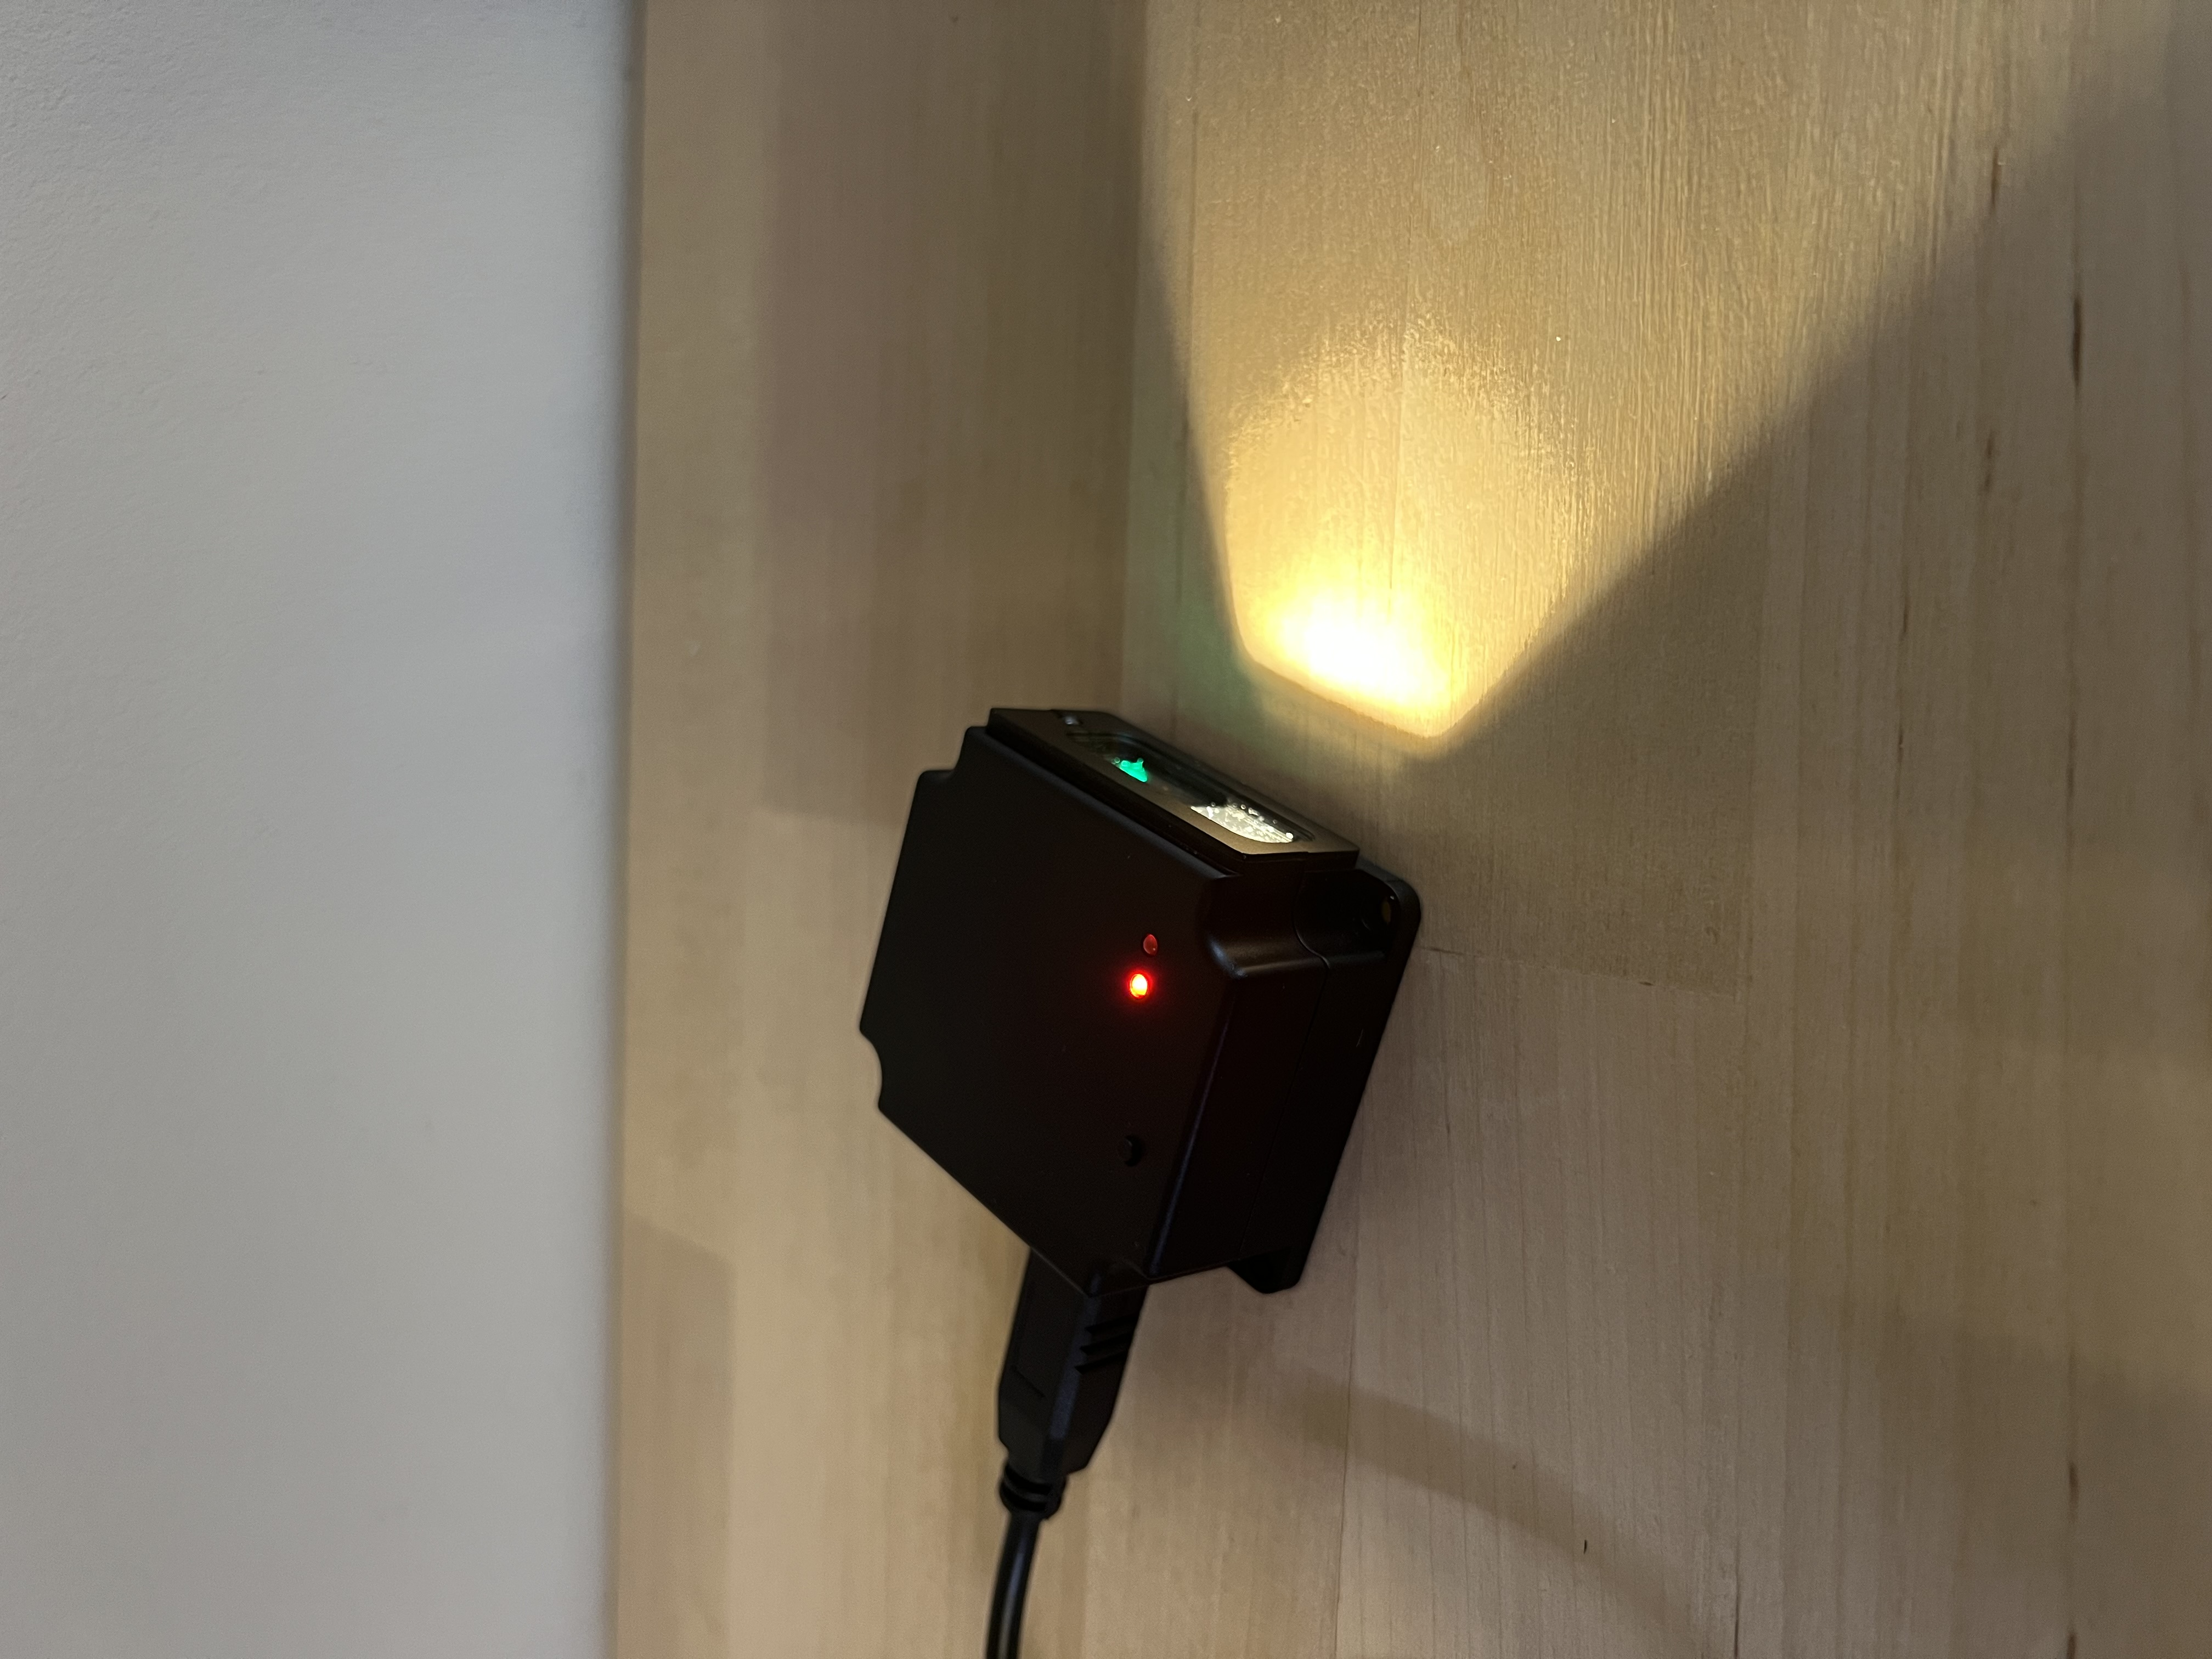
\includegraphics[width=\textwidth]{graphics/F26_scanner_side.jpeg}}
        \caption{Zijaanzicht QR-scanner}
        \label{fig:scannerSide}
    \end{minipage}
\end{figure}

\begin{figure}[h]
    \centering
    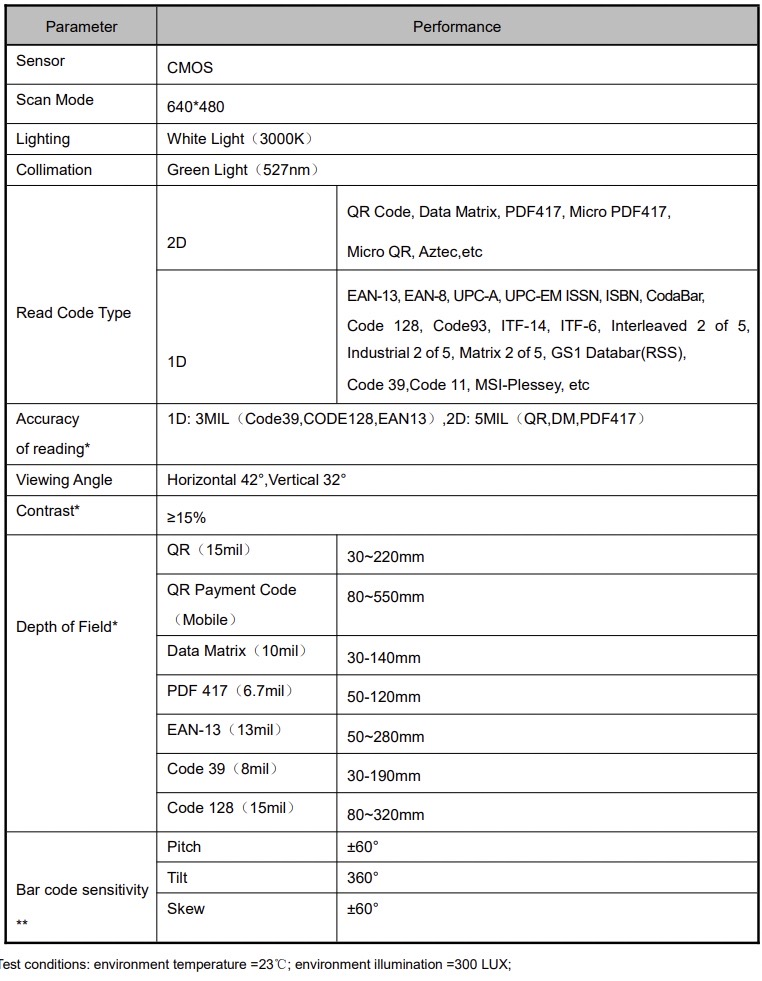
\includegraphics[width=0.8\textwidth]{graphics/F29_aangekochteQRScannerHandleiding.jpg}
    \captionsetup{justification=centering, singlelinecheck=false}    
    \caption{Handleiding aangekochte QR-code scanner.}
    \label{fig:handleidingNieuweQRScanner}
\end{figure}}

Om het experiment van de nieuwe QR-scanner zo goed mogelijk uit te voeren heb ik een nieuw script geschreven, dit script staat vermeld in listing \ref{lst:nieuweQR-codeData}. Deze gaat op dezelfde manier te werk als de huidige QR-code camera en gaat achteraf ook de opgehaalde data opslaan in een \ac{XLSX} bestand. Aan de hand van deze bestanden kunnen we de oude software en hardware vergelijken met de nieuwe om een duidelijke conclusie te maken in het hoofdstuk verwerking van resultaten.

\newpage

\begin{lstlisting}[language=Python, caption={Python script voor experiment van nieuwe QR-code scanner.}, label=lst:nieuweQR-codeData, numbers=left]
    import serial
    import time
    import pyzbar.pyzbar as pyzbar
    from datetime import datetime
    from datetime import timedelta
    from openpyxl import Workbook
    
    # De code opent de seriele poort van de scanner, in dit geval '/dev/tty.usbmodem2027300413411', op een baudrate van 9600
    port = '/dev/tty.usbmodem2027300413411'
    baud = 9600
    ser = serial.Serial(port, baud, timeout=1)
    
    # De variabele 'counter' houdt bij hoeveel QR-codes gescand zijn. De starttijd wordt vastgelegd met datetime.now().
    counter = 1
    start_time = datetime.now()
    
    # Een nieuw werkboek wordt aangemaakt met openpyxl.
    workbook = Workbook()
    worksheet = workbook.active
    
    # De eerste rijen van het werkblad krijgen labels voor de kolommen.
    worksheet['A1'] = 'Counter'
    worksheet['B1'] = 'Timestamp'
    worksheet['C1'] = 'Data'
    
    # Er wordt een while loop uitgevoerd die stopt nadat er 10 QR-codes zijn gescand.
    while counter <= 8:
        # De scanner leest de QR-code en de data wordt in de variabele 'data' opgeslagen.
        data = ser.readline().rstrip()
        if data:
            # De data wordt gedecodeerd met UTF-8 en opgeslagen in de variabele 'message'.
            message = data.decode('utf-8')
            # De huidige tijd wordt vastgelegd met datetime.now().
            timestamp = datetime.now()
            # De verstreken tijd sinds het begin van het scannen wordt berekend.
            elapsed_time = timestamp - start_time
            # Er wordt een datetime object aangemaakt met de huidige datum en de verstreken tijd.
            midnight = datetime.combine(datetime.today(), datetime.min.time())
            elapsed_datetime = midnight + elapsed_time
            # De tijd wordt in een leesbaar formaat opgeslagen in de variabele 'timestamp_str'.
            timestamp_str = elapsed_datetime.strftime('%H:%M:%S:%f')[:-3]
            # De data wordt geprint op het scherm.
            print(f'{counter} | {timestamp_str} | Data: {message}')
            # De data wordt toegevoegd aan het werkblad.
            worksheet.append([counter, timestamp_str, message])
            # De teller wordt verhoogd met 1.
            counter += 1
    
    # Het werkblad wordt opgeslagen als 'qr_codes_records_scanner.xlsx'.
    workbook.save('qr_codes_records_scanner_beschadigd_kaartje_120lux.xlsx')
    # De eindtijd van het scannen wordt vastgelegd met datetime.now() en geprint op het scherm.
    end_time = datetime.now()
    print(f"Counter reached {counter - 1}. Exiting program. Final time of scanning: {end_time - start_time}")
\end{lstlisting}

\subsection{Resultaten nieuwe QR-scanner experiment}
\label{sec:nieuweUitwerkingExperiment}

Hieronder bevinden zich de tabellen met daarin de eindresultaten van het experiment met de nieuwe QR-scanner. Er zijn telkens 50 QR-codes gescand met uitzondering van QR-codes in de beschadigde situatie.

\begin{table}[h]
    \centering
    \begin{tabular}{ c|c|c|c }
        \cline{2-4}
        & \textbf{\textit{QR-code op papier}} & \textbf{\textit{QR-code op gsm}} & \textbf{\textit{Verlichtingssterkte}} \\
        \cline{2-4}        
        \hline
        \textbf{\textit{1. Normaal}} & 157.496 s & 176.180 s & 120 lux \\
        \hline
        \textbf{\textit{2. Lichtinval}} & 177.737 s & 186.605 s & 100000 lux \\
        \hline
        \textbf{\textit{3. Donker}} & 158.847 s & 161.284 s & 5 lux \\
        \hline        
    \end{tabular}
    \captionsetup{justification=centering}
    \caption{De waarden in de tabel zijn uitgedrukt in seconden (s). Geef de resultaten weer van de nieuwe QR-scanner experiment.}
    \label{tab:3expeQR-scanner}
\end{table}

Het experiment dat beschadigde QR-codes omvat zal doorgaan met een set van acht QR-codes die beschadigd of onleesbaar gemaakt zijn. Deze QR-codes zijn zichtbaar op figuur \ref{fig:beschadigdeQR-codes} en zijn gerangschikt op basis van toenemende mate van beschadiging.

\begin{table}[h]
    \centering
    \begin{tabular}{ c|c }
        \cline{2-2}
        & \textbf{\textit{Beschadigd}} \
        \cline{2-2}
        \textbf{\textit{QR-code 1}} & 3,777 s \
        \cline{2-2}
        \textbf{\textit{QR-code 2}} & 11,953 s \
        \cline{2-2}
        \textbf{\textit{QR-code 3}} & 14,995 s \
        \cline{2-2}
        \textbf{\textit{QR-code 4}} & 14,995 s \
        \cline{2-2}
        \textbf{\textit{QR-code 5}} & 22,390 s \
        \cline{2-2}
        \textbf{\textit{QR-code 6}} & 25,340 s \
        \cline{2-2}
        \textbf{\textit{QR-code 7}} & 29,454 s \
        \cline{2-2}
        \textbf{\textit{QR-code 8}} & 32,495 s \
        \cline{2-2}
    \end{tabular}
    \captionsetup{justification=centering}
    \caption{De waarden in de tabel zijn uitgedrukt in seconden (s). De verlichtingssterkte bij deze uitwerking is 120 lux. De QR-codes in kwestie zijn te vinden in figuur \ref{fig:beschadigdeQR-codes}.}
    \label{tab:omgezette_tabel2}
\end{table}

\newpage

\section{Ontwikkeling van chatbot}%

De chatbot maken was een uitdaging binnen de requirements analyse en de tijdslimiet van deze bachelorproef. Echter wou ik deze wel uitwerken zodat er een QR-code op de eenvoudigste manier kan gerecupereerd worden. Om dit doel te bereiken waren twee eigenschappen enorm belangrijk. Een gebruiksvriendelijke interface hanteren alsook een makkelijke integratie in eender welk mediaplatform is noodzakelijk. Met deze twee cruciale kenmerken in het achterhoofd, ben ik naar chatbot platformen gaan zoeken. Veel bedrijven zoals Google of Microsoft bieden interessante dienstverleningen aan om een eigen chatbot te ontwikkelen, maar de prijsklasse van deze platformen ligt buiten het opgegeven budget.

Het zoeken van een chatbot service die aan de vooraf opgestelde eisen en voorwaarden voldoet, was niet eenvoudig. Voor deze Proof-Of-Concept heb ik de service genaamd ‘BotPress’ gekozen. BotPress maakt gebruik van Node.js en een modulaire architectuur. Dit maakt het ons eenvoudiger aangezien de business logica en de back-end van de Lockit Rentals applicatie ook gecodeerd is in dezelfde taal. Het biedt ook functies aan, zoals machine learning, natuurlijke taalverwerking, contextuele dialoogbeheer, integratie met externe services en analyse van gebruikersgedrag. Dit alles binnen een gratis opstartkost met maximaal 1000 conversaties per maand. Dankzij deze voordelen kunnen we de kennis verder zetten en de aangepaste modules integreren.

Het gebruik van BotPress is eenvoudig maar kan indien nodig voor genoeg diepgang zorgen. De conversatie of workflow bestaat uit verschillende blokken wat ‘Nodes’ wordt genoemd. Hierin kunnen vijf types van acties gebeuren zoals weergegeven in figuur \ref{fig:botpressActies}. Als eerste actie kan de eindgebruiker een voorgeprogrammeerd bericht ontvangen. Dit bericht kan uit verschillende types bestaan: tekst, video, audio, afbeeldingen of locatie zijn hier voorbeelden van. In een tweede actie binnen een Node blok kan er een interactie aangegaan worden met de eindgebruiker. Bij deze optie kan of mag de gebruiker een antwoord geven op een vooraf gedefinieerde vraag. Dit antwoord wordt nadien bewaard in een variabele die aangemaakt is binnen de workflow figuur \ref{fig:botpressVariables}. Het laten uitvoeren van eigen geschreven of \ac{AI} gegenereerde code is de derde actie die binnen de werkomgeving kan worden aangemaakt. Dit laat toe om opdrachten uit te sturen naar andere externe diensten buiten het platform. Bij de implementatie van de Lockit Rentals Chatbot maken wij hier uitgebreid gebruik van om te kunnen communiceren met de Lockit Rentals applicatie. De voorlaatste stap markeert de overgang tussen verschillende 'Nodes', waarbij er meerdere mogelijkheden zijn om verder te gaan met het gesprek. Hierdoor krijgt de eindgebruiker de vrijheid om verschillende routes te verkennen en het gesprek verder op maat te maken om zoveel mogelijk informatie te vergaren. De laatste actie die het minst gebruikt is binnen onze toepassing is een \ac{AI} task. 
Belangrijk om weten is dat er geen beperkingen zijn met betrekking tot de volgorde waarin de vijf acties uitgevoerd worden. Aan de hand van een gestructureerd stroomdiagram heb ik de chatbot opgebouwd weergegeven in figuur \ref{fig:workflowBotPress}. 

\subsection{Stappen om QR-code terug te winnen via chatbot}

Hieronder volgt een voorbeeld hoe je als festivalganger een QR-code kan terugwinnen via de chatbot. Deze stappen worden later gevisualiseerd in sectie \ref{sec:resultatenChatbot}.
\newline

Primaire actor: Festivalganger die zijn of haar locker niet kan openen vanwege een verloren QR-code.
\newline
Secundaire actor: Chatbot dat is ontworpen om de festivalganger te helpen de verloren QR-code terug te geven.
\newline
Normaal verloop:

\begin{enumerate}
    \item De festivalganger typt een bericht om de chatbot te activeren.
    \item De festivalganger selecteert de optie "verloren QR-code".
    \item De chatbot haalt de huidige festivals op waar de lockers actief staan en presenteert deze aan de festivalganger via een keuze menu. \ref{ophalenActieveFestivals}
    \item De festivalganger selecteert het juiste festival waarbij hij/zij de locker heeft aangekocht.
    \item De chatbot vraagt naar het e-mailadres van de festivalganger om de QR-code op te sturen.
    \item De festivalganger verstrekt het juiste e-mailadres.
    \item De chatbot stuurt een verzoek naar de achterliggende service met het zonet ingegeven emailadres. \ref{versturenRequestEmail}
    \item Het systeem zal de QR-code ophalen en een mail versturen. \ref{ophalenQR}
    \item De chatbot krijgt het antwoord van het verzoek binnen en geef een gepaste melding.
    \item De festivalganger ontvangt de QR-code en kan deze gebruiken om zijn of haar locker te openen.
\end{enumerate}

Alternatieve verlopen:
\newline
Hierbij zal de chatbot een gepaste foutmelding geven en de vraag opnieuw stellen. De chatbot zal er alles aan doen om de eindgebruiker genoeg informatie te verschaffen zodanig dat hij/zij zijn weg vindt in de conversatie.

\subsection{Ophalen evenementen waarop lockers actief zijn}
\label{ophalenActieveFestivals}
De chatbot zal de vraag stellen om een evenement aan te duiden in de chat. Een lijst van alle actieve evenementen waarop de lockers actief staan is hiervoor nodig. Deze actie wordt uitgevoerd in een stroomdiagram aan de hand van eigen geschreven code. Het antwoord op dit verzoek wordt bewaard in vooraf gedefinieerde lijsten. Deze code is voorgesteld in listing \ref{lst:botpressActie1}.

\begin{lstlisting}[language=Python, caption={Code blok geschreven in javascript om een actie van botpress uit te voeren.}, label=lst:botpressActie1, numbers=left]
    const response = await axios.get('https://europe-west2-lockit-testing.cloudfunctions.net/getActiveShops')
    
    const festivalsToAdd = response.data.map((festival) => festival.name)
    console.log(festivalsToAdd)
    // add the new festivals to the list
    workflow.ListOfFestivals = festivalsToAdd
    workflow.ListOfFestivalsObj = response.data
\end{lstlisting}

De ophaling van alle actieve evenementen verloopt in de backend van de Lockit Rentals applicatie. Dit wordt geconverteerd naar duidelijke objecten om zo weer te geven in de chat.
Methode \ref{lst:botpressActie2}, waarin men informatie verkrijgt van festivals waar lockers actief staan.
\begin{lstlisting}[language=JavaScript, caption={Methode waarin festivals worden ogpehaald waar lockers actie zijn.}, label=lst:botpressActie2, numbers=left]
    import * as functions from 'firebase-functions';
    import * as admin from 'firebase-admin';
    
    export const shopOverview = functions
    .region('europe-west2')
    .https.onRequest(async (req, resp) => {
        const db = admin.firestore();
        
        const activeShops = await db
        .collection('shop')
        .where('status', '==', 'LIVE')
        .get();
        
        resp
        .status(200)
        .send(activeShops.docs.map((doc) => ({ id: doc.id, ...doc.data() })));
    });
\end{lstlisting}

\subsection{Verzoek sturen naar backend om verloren QR-code op te halen}
\label{versturenRequestEmail}

Eénmaal de chatbot het e-mailadres goed heeft ontvangen kan het proces van het terugwinnen van een QR-code in werking treden. De chatbot voert een taak uit dat weergegeven wordt in listing \ref{lst:botpressActie3}. 

\begin{lstlisting}[language=JavaScript, caption={Een blok uitvoerbare code geschreven in javascript in een actie van Botpress. Deze code zal een verzoek uitsturen en het antwoord hiervan capteren.}, label=lst:botpressActie3, numbers=left]
    const response = await axios
    .post('https://europe-west2-lockit-testing.cloudfunctions.net/recoverLostCode', {
        shopId: workflow.FestivalNameObj['id'],
        email: workflow.Emailadress
    })
    .then((response) => {
        workflow.EmailSend = true
    })
    .catch((error) => {
        if (error.response && error.response.status === 404) {
            workflow.RecoveQr = "I couldn't find any email address associated with a purchased QR code. Please try again."
        } else if (error.response && error.response.status === 500) {
            workflow.RecoveQr = 'Something bad happend..... :^('
        } else {
            console.log(error)
        }
    })
\end{lstlisting}

\subsection{Ophalen van QR-code en aanmaken e-mail}
\label{ophalenQR}

Dit verzoek zal opnieuw afgehandeld worden in de backend van de Lockit Rentals applicatie. Het uitvoeren van onderstaande code \ref{lst:botpressActie4} zal de QR-code ophalen uit de reservatie tabel. Het antwoord waarin hij aangeeft dat de QR-code succesvol is opgehaald en de herstel email zullen verzonden worden. Op deze manier kan de chatbot een gepaste actie voorzien om de gebruiker erop te wijzen dat deze email onderweg is. 

\begin{lstlisting}[language=JavaScript, caption={Het ophalen van de bijhorende QR-code, indien dit gelukt is, opmaken en bewaren in de databank.}, label=lst:botpressActie4, numbers=left]
    const shopSnap = await db.collection('shop').doc(recoveryData.shopId).get();
    
    /**
    * If we can't find the shop, no point in searching for the reservation
    */
    if (!recoveryData.shopId || !shopSnap.data()) {
        resp.status(500).send();
    }
    
    if (recoveryData.email) {
        const reservationsSnap = await shopSnap.ref
        .collection('reservations')
        .withConverter(converter<ShopReservation>())
        .where('customerEmail', '==', recoveryData.email)
        .get();
        for (const reservationSnap of reservationsSnap.docs) {
            const reservation: ShopReservation = reservationSnap.data();
            await db
            .collection('mail')
            .doc()
            .create({
                to: reservation.customerEmail,
                message: {
                    subject: '🎉 Your locker for ' + reservation.shopName,
                    html: constructLiveSaleEmail(
                    reservation.lockerNumber + '',
                    reservation.optionName,
                    reservation.shopName,
                    reservation.customerName,
                    reservation.lockerType,
                    reservation.optionLocationName,
                    reservation.accessCode + ''
                    ),
                },
            });
        }
        if (reservationsSnap.size > 0) {
            resp.status(201).send();
        } else {
            resp.status(404).send('email adress not found');
        }
    } else if (recoveryData.phone) {
        console.log('tel reached');
    }
    
    resp.status(200).send();
});
\end{lstlisting}

\subsection{Versturen van aangemaakte herstel email}
\label{versturenQRcode}

Om de aangemaakte email met daarin de gerecupereerde QR-code te verzenden naar de eindgebruiker is echter een ander verhaal. De aangemaakte email wordt bewaard in een tabel ‘customerEmail’. Om deze mail automatisch te detecteren gebruiken we de extentie binnenin Firebase genaamd ‘Tigger email’. Deze extentie zorgt voor het detecteren van emails die aangemaakt zijn binnen de tabel ‘customerEmail’. De extentie kan zo nog een derde provider aanspreken genaamd ‘Mail Sender’ die ervoor zal zorgen dat de email naar de desbetreffende correspondent verstuurd wordt \ref{fig:resultaatEmailSender}. Via deze tool kunnen we alles analayseren wat er precies gebeurt met de verstuurde email. 

\begin{figure}[h]
    \centering
    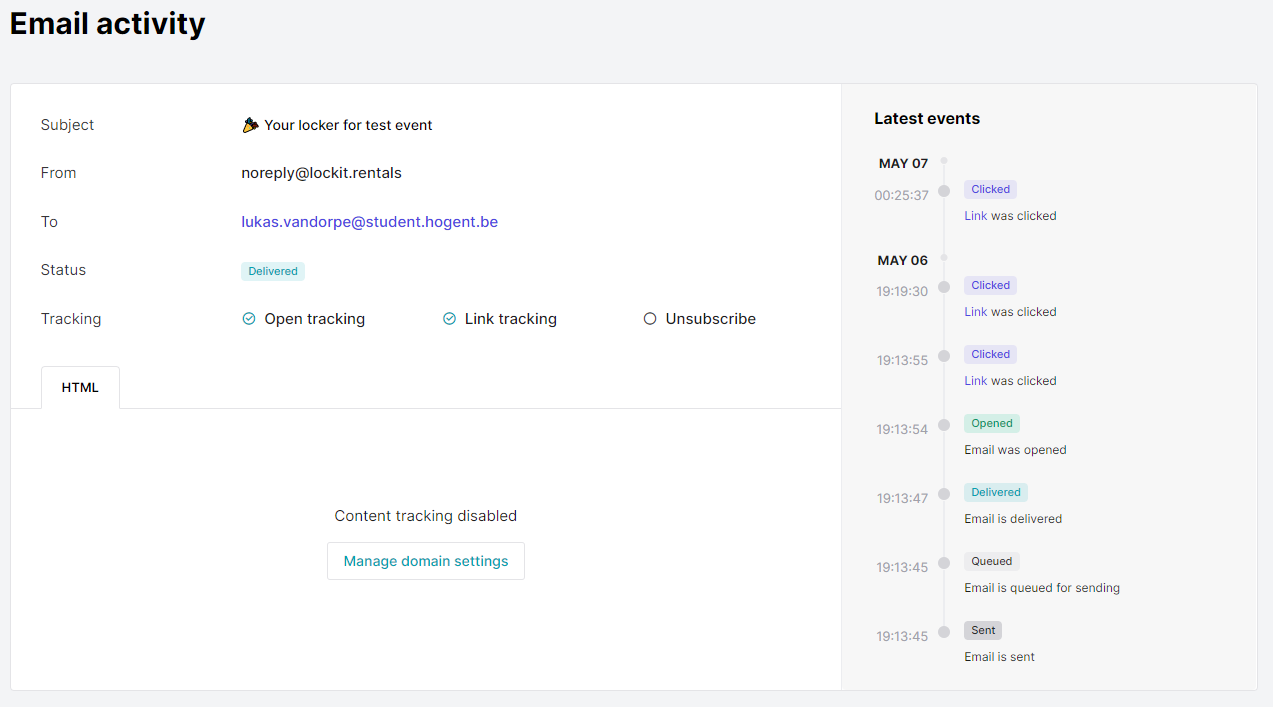
\includegraphics[width=0.8\textwidth]{graphics/F35_mailSender.png}
    \captionsetup{justification=centering,singlelinecheck=false}
    \caption{De tool 'Mail Sender' waarop we de verzonden mail kunnen traceren.}
    \label{fig:resultaatEmailSender}
\end{figure}


\begin{figure}[h]
    \centering
    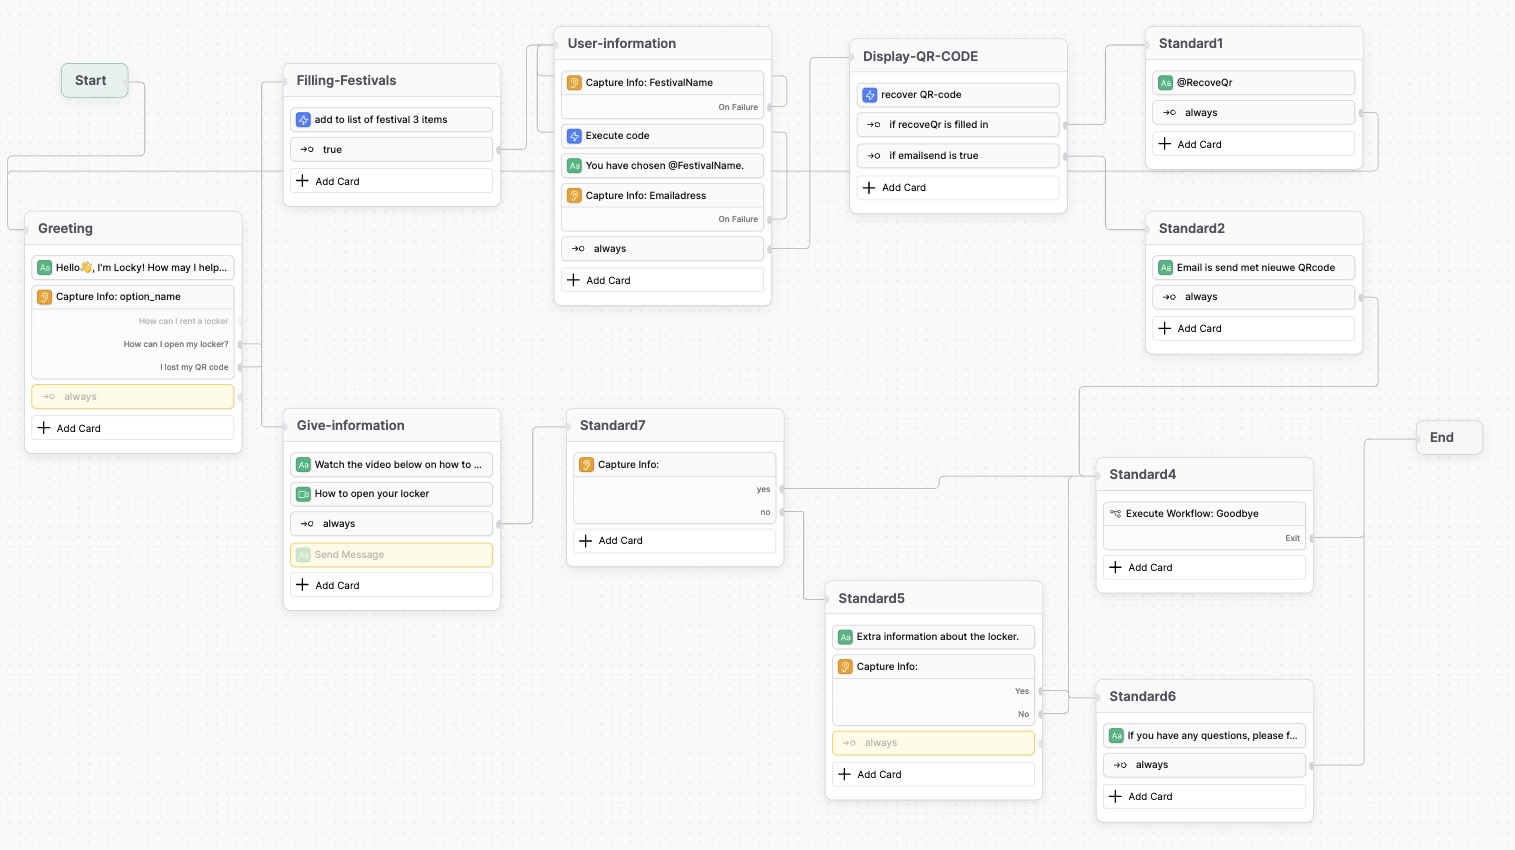
\includegraphics[angle=90, width=0.9\textwidth]{graphics/F36_workflowBotPress.jpg}
    \captionsetup{justification=centering}    
    \caption{De workflow van de Lockit Rentals Bot gemaakt in BotPress.}
    \label{fig:workflowBotPress}
\end{figure}

%todo: figuur aanvullen van volledig model botpress
\begin{figure}[h]
    \centering
    \begin{minipage}{0.45\textwidth}
        \centering
        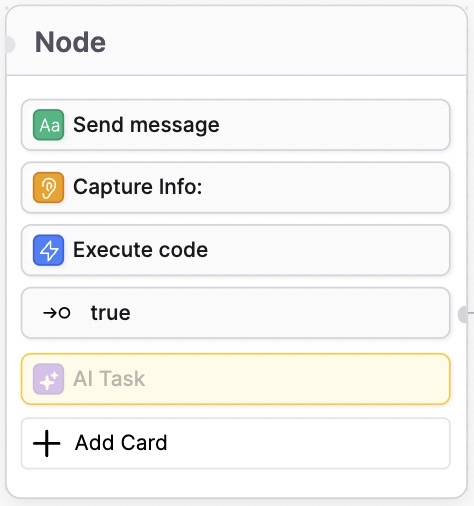
\includegraphics[width=\textwidth]{graphics/F31_botpress_Acties.jpg}
        \caption{Representatie BotPress Node en vijf verschillende acties.}
        \label{fig:botpressActies}
    \end{minipage}
    \hfill
    \begin{minipage}{0.45\textwidth}
        \centering
        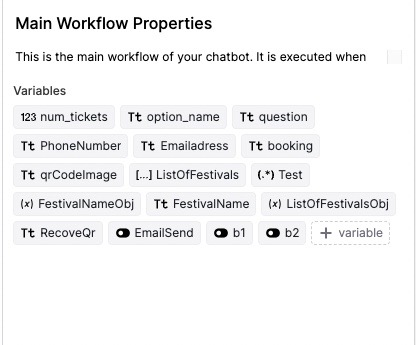
\includegraphics[width=\textwidth]{graphics/F32_botpress_Variables.jpg}
        \caption{Alle variabelen die binnen de workflow zitten voor de Lockit Rentals chatbot.}
        \label{fig:botpressVariables}
    \end{minipage}
\end{figure}















%%=============================================================================
%% Verwerking resultaten
%%=============================================================================

\chapter{Verwerking resultaten}%
\label{ch:verwerkingresultaten}

In dit hoofdstuk zullen de resultaten van de experimenten aangehaald worden. De nieuwe ontwikkelde chatbot met al zijn vereiste functionaliteiten zal ook aan bod komen. Op basis van deze gegevens en uitvoeringstijden wordt er zo tot een correct antwoord gekomen op de hoofdonderzoeksvraag in sectie \ref{sec:Hoofdonderzoeksvragen}.


\section{Resultaten QR-code scanners}
\label{sec:resultatenQR-codeScanners}

In tabellen \ref{tab:3expeQR-camera}, \ref{tab:omgezette_tabel_seconds}, \ref{tab:3expeQR-scanner} en \ref{tab:omgezette_tabel2} zijn de uitvoeringstijden van de verschillende QR-code lezers waar te nemen. Als eerste schetsen we een algemeen beeld om nadien dieper in te gaan op de omgeving en de factor die de leesbaarheid en leessnelheid kan beïnvloeden. 

Hieronder vindt u per gehanteerde scan een overzicht van het gemiddelde, de mediaan, de standaardafwijking en de variatiecoëfficiënt van alle metingen. De meting over de beschadigde QR-codes zijn niet in acht genomen bij dit besluit. Deze komen verder aanbod.


\begin{table}[h]
    \centering
    \begin{tabular}{ |c|c|c| }
        \hline
        \multicolumn{1}{|c|}{} & \textbf{Oude QR-camera} & \textbf{Nieuwe QR-scanner} \\       
        \hline
        \textbf{\textit{Gemiddelde}} & 267,832s & 168,635s \\
        \hline
        \textbf{\textit{Mediaan}} & 217,566s & 176,180s \\
        \hline        
        \textbf{\textit{Standaardafwijking}} & 132,079s & 28,778s \\
        \hline
        \textbf{\textit{Variantiecoëfficiënt}} & 0,493 & 0,018 \\
        \hline
    \end{tabular}
    \captionsetup{justification=centering}
    \caption{De waarden in de tabel zijn uitgedrukt in seconden (s). Geven de statische gegevens terug van uitgevoerde experimenten.}
    \label{tab:nieuweScanner}
\end{table}

    
Door naar de statistische gegevens verder te kijken, kunnen we besluiten dat de nieuwe scanner beter scoort dan de oude QR-scanner op vlak van uitlezen en detecteren van een QR-code. Aangezien wij hier gewerkt hebben met totale tijdswaarden van één specifieke omgeving en één specifiek type kunnen we geen effectieve vergelijking geven tussen de verschillende factoren. We kunnen hieruit wel concluderen welke scanner er algemeen beter werkt in de geteste omgevingen en situaties.

Uit de resultaten van huidige QR-camera experiment kunnen we nog enkele conclusies nemen. Als enige tester heb ik mij zoveel mogelijk gedragen zoals een huurder de QR-code zou scannen. Wat ik vooral opmerkte bij het scannen van toegangscodes bij de huidige camera is dat de QR-code op een perfecte afstand moet gescand worden. Er kan absoluut niet afgeweken worden van de oriëntatie hoek bij het scannen. Hierdoor kunnen we concluderen dat de huurder een duidelijke indicatie moet krijgen waar en op welke afstand hij/zij de QR-code moet houden. Dit probleem was totaal niet het geval bij de nieuwe scanner opstelling. De herkenningssoftware kon nog steeds de data uitlezen ook al hield je de toegangscode in verschillende posities.

Uit geteste omgevingen en soorten weergave van QR-codes zien we dat de QR-code op gsm algemeen beter scoort dan de QR-codes weergegeven op papier. De helderste witruimtes tussen de pixels van de aangemaakte QR-code zorgen voor een beter contrast tijdens het detecteren van de code. Vandaar dat de huidige QR-code camera in een donkere omgeving zo slecht scoort. Er is weinig licht aanwezig om het contrast genoeg te benadrukken. 

Uit de experimenten met de beschadigd QR-codes kunnen we het volgende concluderen. Na het scannen van QR-code 4 weergegeven in \ref{tab:omgezette_tabel_seconds} slaagde de huidige QR-code camera er niet meer in om volgende QR-codes te detecteren. De QR-codes zijn op sommige belangrijke onderdelen teveel beschadigd. De gespecialiseerde QR-code scanner daarentegen kan de beschadigde QR-codes beter en sneller detecteren \ref{tab:omgezette_tabel2}. Dit bevestigt dat het herkenningsalgoritme op de USB camera minder geschikt is voor het uitlezen van beschadigde QR-codes ten opzichte van de nieuwe aangekochte scanner.
\newpage
\section{Bevindingen  chatbot}
\label{sec:resultatenChatbot}

Door het gebruik van een zeer recent chatbot platform zijn er tijdens ontwikkeling een paar obstakels opgedoken. Aangezien dit platform onlangs een volledige hervorming heeft doorstaan, was dit moeilijk om de juiste informatie te vinden hoe een chatbot ontwikkeld kan worden in BotPress. De documentatie over het gebruik was omslachtig en heel basisgericht. 

Zoals al aangegeven in de sectie \ref{sec:stappenChatbot} van Proof-Of-Concept heb ik kunnen aantonen dat een chatbot op een gebruiksvriendelijke en handige manier de verloren QR-codes kan genereren. De herstelmail wordt weergegeven in figuur \ref{fig:resultatEmailQR-code}. De chatbot is ook in staat om informatie terug te geven naar believen van de eindgebruiker. Het is echter zeer moeilijk om de gebruiker zijn vragen te capteren en de eindgebruiker naar het juiste keuzemenu te leiden. Hieronder zijn de negatieve en postieve punten opgesomd op basis van mijn ontwikkelingstijd en ervaringen op het platform.

Het eerste pluspunt dat ik dit platform kan geven is de manier waarop het gebouwd is en welke integratiemogelijkheden dit aanbiedt. Eén van de requirments gaf aan dat de chatbot zich onafhankelijk moest situeren. Het platform dient als eindpunt en heeft niets te maken met de huidige operaties in het locker verhuur proces. Een tweede pluspunt is de eigenschap van eigengeschreven code uit te voeren waar en wanneer je dit wilt. Dit gegeven is zeldaam als er gekeken wordt naar grote technologiegiganten op vlak van geautomatiseerde chatbots. 
Het ontwikkelen van een chatbot puur voor specifieke acties zoals het terughalen van QR-codes zou ook uitgevoerd kunnen worden aan de hand van een versimpeld formulier. Door het gebruik van een betere en grotere techniek dan nodig, laten we de mogelijkheid open om aan uitbreidingen te doen. Een volgend positief element is de manier van integratie tussen verschillende services. Deze mogelijkheden waren zeer goed uitgewerkt en gedocumenteerd waardoor integratie vlekkeloos verliep. Door deze pijlers mee te nemen in onderzoek en ontwikkeling impliceert dit onze gemaakte keuze van de tool BotPress.

De negatieve elementen waren vooral de leercurve van de toepassing. Deze toepassing doet veel achter de schermen waardoor de logica moeilijk te vatten was van een puur technisch gericht perspectief. De documentatie dat niet optimaal is noch de informatie die gepubliceerd was door anderen verhoogt de moeilijkheidsgraad. De negatieve elementen zijn eerder de opsomming van zeer kleine ontbrekende elementen die aanslepen en weerspiegelen zich in gevolgen van de eindgebruiker. Een voorbeeld hiervan is dat de eindgebruiker zelf interactie moet opstarten met de chatbot.

Doordat de drie eigenschappen kostprijs, integratie en afhankelijkheid toch weer te vinden zijn in dit platform kan geconcludeerd worden dat deze tool voldoende was om de doelstelling te bereiken. BotPress kan zeker gezien worden als een stabiel chatbot platform bij verder gebruik en ontwikkeling. Ook bij verdere ontwikkeling van de gemaakte Proof-Of-Concept zie ik de Lockit Rentals chatbot verder doorgroeien.



\begin{figure}[h]
    \centering
    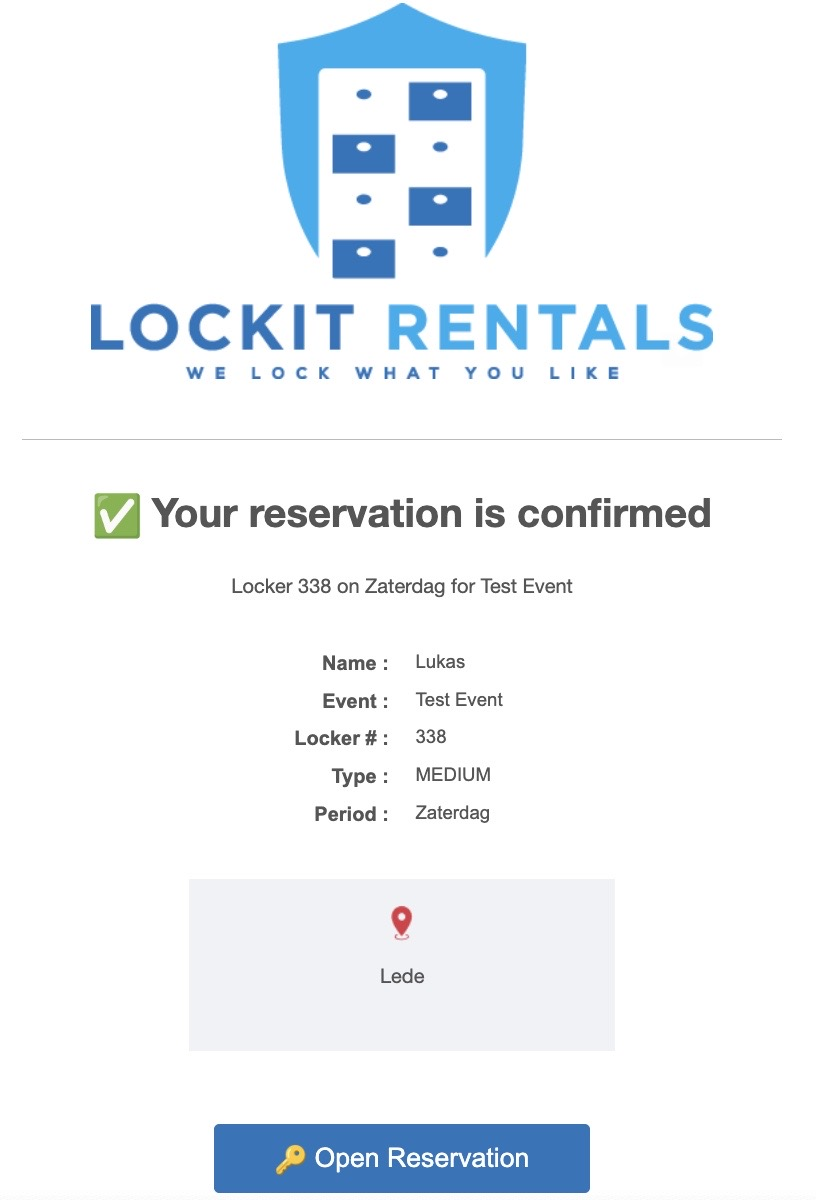
\includegraphics[width=0.5\textwidth]{graphics/F34_mailQR-code.jpg}
    \captionsetup{justification=centering, singlelinecheck=false}
    
    \caption{Een verstuurde mail afkomstig van Lockit Rentals met in bijlage de teruggewonnen QR-code.}
    \label{fig:resultatEmailQR-code}
\end{figure}















% Voeg hier je eigen hoofdstukken toe die de ``corpus'' van je bachelorproef
% vormen. De structuur en titels hangen af van je eigen onderzoek. Je kan bv.
% elke fase in je onderzoek in een apart hoofdstuk bespreken.



%\input{...}
%\input{...}
%...

%%=============================================================================
%% Conclusie
%%=============================================================================

\chapter{Conclusie}%
\label{ch:conclusie}

% TODO: Trek een duidelijke conclusie, in de vorm van een antwoord op de
% onderzoeksvra(a)g(en). Wat was jouw bijdrage aan het onderzoeksdomein en
% hoe biedt dit meerwaarde aan het vakgebied/doelgroep? 
% Reflecteer kritisch over het resultaat. In Engelse teksten wordt deze sectie
% ``Discussion'' genoemd. Had je deze uitkomst verwacht? Zijn er zaken die nog
% niet duidelijk zijn?
% Heeft het onderzoek geleid tot nieuwe vragen die uitnodigen tot verder 
%onderzoek?

In dit onderzoek wordt een antwoord gegeven op de onderzoeksvraag: “Welke technologieën kan het bedrijf Lockit Rentals toepassen om hun bedrijfsactiviteiten bij het verhuren van lockers te optimaliseren?”. Verder geven de deelonderzoeksvragen een duiding welke probleemstellingen er in dit onderzoek behandeld moeten worden. Er is ingespeeld op de eisen die vooraf zijn opgesteld zowel voor het zoeken naar optimalisatie van het scanproces alsook voor het terugwinnen van de verloren of beschadigde QR-codes. \newline
Het bestuur van Lockit Rentals heeft aangehaald dat de QR-scanner een onderdeel was van het smart locker systeem dat nog niet op punt stond. Deze potentiële problemen worden als storend ervaren bij de huurders. De eerste doelstelling was om de leessnelheid en nauwkeurigheid van QR-code scanners te verbeteren. Onderzoek duidt aan dat het gebruik van gespecifieerde QR-code scanner een positieve invloed kon voortbrengen. Bij eigen experimenten kan deze stelling bekrachtigd worden. Een QR-code scanner ten opzichte van een QR-code camera met eigen herkenningsalgoritme kan betere QR-codes  uitlezen en verwerken. De resultaten tonen aan dat het uitlezen van QR-codes in een donkere omgeving een uitdaging vormt. Daarom moet kunstmatig licht altijd aanwezig zijn als we op alle momenten van de dag willen scannen. Beschadigde QR-codes kunnen uitgelezen worden door gespecialiseerde QR-code scanners. Maar in vergelijking met de huidige camera merken we op dat dit herkenningsalgoritme niet voldoende op punt staat om beschadigde QR-codes te detecteren.\newline
Niet alleen kunnen we dit concluderen op vlak van experimenten maar ook op vlak van functionaliteit die de huidige QR-camera niet bezit. Zo heeft de nieuwe QR-scanner veel configuratiemogelijkheden die de gewone USB camera niet heeft. Een belangrijke configuratie is de eventuele eigen kunstmatige lichtbron ter hoogte van de lens, hierdoor zal de getoonde QR-code een beter contrast geven tussen de pixels van de QR-code. Dit contrast brengt positieve invloed op de leessnelheid. Ook zijn allerlei detectie snelheden en fouttoleratie configuraties toepasbaar op de nieuwe QR-scanner, op deze manier kan de scanervaringen van de festivalgangers aangenamer gemaakt worden.
\newline
Om de verloren QR-code terug te winnen is er gefocust op de vooraf gemaakte eisen van Lockit Rentals. Het was duidelijk dat het ontwerpen van een geautomatiseerde chatbot een geschikte oplossing zou zijn. Het maken van een chatbot kan echter heel tijdrovend zijn. De gebruikte chatbot service BotPress is in dit onderzoek gehanteerd. Deze is gekozen voor zijn positieve aspecten dat overeenstemmen met de opgelegde eisen. BotPress is gratis te gebruiken voor een bepaald aantal verstuurde berichten, het geeft veel vrijheid naar de ontwikkelaar en het is makkelijk te integreren op andere platformen.\newline
De gemaakte chatbot toont aan dat deze een perfecte oplossing biedt voor het terugwinnen van QR-codes en voor het verschaffen van praktische hulp ten behoeve van de eindgebruiker. Deze conclusies zijn gebaseerd op de specifieke omstandigheden waarin de verkoop uitsluitend online plaatsvindt. Als men toegangscodes zal verkopen op papier zal het terugwinnen van verloren QR-codes enkel gebeuren door logistieke medewerkers.



%---------- Bijlagen -----------------------------------------------------------

\appendix

\chapter{Onderzoeksvoorstel}

Het onderwerp van deze bachelorproef is gebaseerd op een onderzoeksvoorstel dat vooraf werd beoordeeld door de promotor. Dat voorstel is opgenomen in deze bijlage.

\section*{Samenvatting}
  Dankzij nieuwe technologieën is het huren van een locker op festivals eenvoudig. Bij de locker units van het bedrijf Lockit Rentals kunnen lockers geopend worden met behulp van QR-codes. Deze worden voor aanvang van het evenement online verkocht. QR-codes zijn zo ontworpen dat deze niet kunnen onthouden worden. Wanneer de QR-code scanner moeite heeft met het symbool uit te lezen of bezoekers hun QR-code verliezen, spelen ze hierdoor de toegang tot hun locker kwijt. Implementatie van nieuwe technologieën kan ervoor zorgen dat de QR-code scanners geoptimaliseerd worden. Bij verlies van de toegangscode, kan de huurder rekenen op een geautomatiseerde support chatbot die hun assisteert om verloren QR-codes opnieuw te genereren. Dit resulteert in meer gebruiksgemak naar de klanten toe en minder moeilijkheden tijdens uitbating van lockers.


% Verwijzing naar het bestand met de inhoud van het onderzoeksvoorstel
%%==============================================================================
% Sjabloon onderzoeksvoorstel bachproef
%==============================================================================
% Gebaseerd op document class `hogent-article'
% zie <https://github.com/HoGentTIN/latex-hogent-article>

% Voor een voorstel in het Engels: voeg de documentclass-optie [english] toe.
% Let op: kan enkel na toestemming van de bachelorproefcoördinator!
\documentclass{hogent-article}

% Invoegen bibliografiebestand
\addbibresource{voorstel.bib}

% Informatie over de opleiding, het vak en soort opdracht
\studyprogramme{Professionele bachelor toegepaste informatica}
\course{Bachelorproef}
\assignmenttype{Onderzoeksvoorstel}
% Voor een voorstel in het Engels, haal de volgende 3 regels uit commentaar
% \studyprogramme{Bachelor of applied information technology}
% \course{Bachelor thesis}
% \assignmenttype{Research proposal}

\academicyear{2022-2023} % TODO: pas het academiejaar aan

% TODO: Werktitel
\title{Ontwikkeling van gebruiksvriendelijke technologieën in het optimaliseren van lockerverhuur}

% TODO: Studentnaam en emailadres invullen
\author{Lukas Van Dorpe}
\email{lukas.vandorpe@student.hogent.be}

% TODO: Medestudent
% Gaat het om een bachelorproef in samenwerking met een student in een andere
% opleiding? Geef dan de naam en emailadres hier
% \author{Yasmine Alaoui (naam opleiding)}
% \email{yasmine.alaoui@student.hogent.be}

% TODO: Geef de co-promotor op


\supervisor[Co-promotor]{S. Vandenhouten (Lockit Rentals,
\href{mailto:sebastien@lockit.rentals}{        sebastien@lockit.rentals})}

%\supervisor[Co-promotor]{W. Van Dorpe (Lockit Rentals, %\href{mailto:wannesvandorpe@hotmail.com}{wannesvandorpe@hotmail.com})}
% Binnen welke specialisatierichting uit 3TI situeert dit onderzoek zich?
% Kies uit deze lijst:
%
% - Mobile \& Enterprise development
% - AI \& Data Engineering
% - Functional \& Business Analysis
% - System \& Network Administrator
% - Mainframe Expert
% - Als het onderzoek niet past binnen een van deze domeinen specifieer je deze
%   zelf
%
\specialisation{Mobile \& Enterprise development}
\keywords{Lockerverhuur, QR-code, Chatbot}

\begin{document}

\begin{abstract}
  Dankzij nieuwe technologieën is het huren van een locker op festivals eenvoudig. Bij de locker units van het bedrijf Lockit Rentals kunnen lockers geopend worden met behulp van QR-codes, deze worden voor aanvang van het evenement online verkocht. QR-codes zijn zo ontworpen dat deze niet kunnen onthouden worden. Wanneer de QR-code scanner moeite heeft met het symbool uit te lezen of bezoekers hun QR-code verliezen, spelen ze hierdoor de toegang tot hun locker kwijt. Implementatie van nieuwe technologieën kan ervoor zorgen dat de QR-code scanners geoptimaliseerd worden. Bij verlies van de toegangscode, kan de huurder rekenen op een geautomatiseerde support chatbot die hun assisteert om verloren QR-codes opnieuw te genereren. Dit resulteert in meer gebruiksgemak naar de klanten toe en minder moeilijkheden tijdens uitbating van lockers.
  
\end{abstract}

\tableofcontents

% De hoofdtekst van het voorstel zit in een apart bestand, zodat het makkelijk
% kan opgenomen worden in de bijlagen van de bachelorproef zelf.
% \input{voorstel-inhoud}


\section{Introductie}%
\label{sec:introductie}

%TODO oplijsting van festival bandjes veranderen

Tegenwoordig staan festivals en evenementen heel ver op het vlak van technologie. Toegangstickets zijn voorzien van QR-codes en kunnen online gekocht worden, geld opladen op festival bandjes waarmee bezoekers overal contactloos kunnen betalen,\dots\space De innovatie om de lockerverhuur op evenementen te digitaliseren en te moderniseren komt vanuit de veranderde noden en behoeften van festivalgangers. Onderzoek zal doeltreffend zijn voor de implementatie van gebruiksvriendelijke technieken bij de verhuur van lockers.

Begin 2022 kwamen de oprichters van Lockit Rentals, Wannes Van Dorpe en Sebastien Vandenhouten, op de markt met nieuwe QR-units. Bij het huren van een locker ontvangt de klant een QR-code die als toegangscode dient voor het openen van een kluisje. Met die unieke QR-code kunnen klanten hun persoonlijke spullen veilig opbergen en de locker onbeperkt openen voor een vaste opgelegde periode. 

Bij Lockit Rentals zijn er twee opties om lockers te verhuren. De eerste mogelijkheid is het verkopen van gedrukte kaartjes met QR-codes aan de kassa. Dit brengt echter hoge personeelskosten met zich mee. Daarnaast kan men ook kiezen om de QR-units standalone uit te baten. Dit houdt in dat Lockit Rentals de units op locatie levert en vanop afstand alles monitort. Hierbij worden de QR-codes online verkocht. De problemen ontstaan als de QR-codes niet meer uitgelezen kunnen worden of wanneer de klant zijn/haar QR-code verliest. Deze problemen kunnen zowel gebaseerd zijn op een fout in de hardware als in de software. Vanuit deze probleemstelling formuleert dit onderzoek een oplossing.  


%---------- Stand van zaken ---------------------------------------------------

\section{State-of-the-art}%
\label{sec:state-of-the-art}

Bij lockerverhuur bestaan er drie verschillende sloten: digitale pincodes, sleutelsloten en vernieuwde technologieën. Als eerste zijn er sloten met een digitale pincode, eventueel gedrukt op een kaartje. Deze zijn erg populair bij festivalgangers aangezien je dit makkelijk kunt onthouden, net zoals een pincode van een smartphone.

De meest eenvoudige manier om persoonlijke bezittingen veilig op te bergen is het kluisje vastmaken met een sleutel. Deze manier van lockeruitbating wordt minder vaak gebruikt op festivals, aangezien het mogelijk is om de sleutel te verliezen. Daarbovenop bestaat er geen mogelijkheid om de locker units standalone te laten draaien wanneer men kiest voor sleutelsloten. 

De laatste jaren zijn nifDeuwe technologieën op de markt gekomen voor het openen van een kluisje. Eén van deze technologieën is het openen van een locker met een vooraf aangemaakte QR-code.


\subsection{QR-codes}}%
\label{sec:QR-codes}

Een QR-code is een machinaal leesbaar optisch label met informatie over het bijhorend product \autocite{Chang2014}. In dit onderzoek is het product de toegangscode voor het openen van een locker. QR-code staat voor \textit{Quick Response code} en is een soort matrix streepjes code \autocite{Tiwari2016}. Het is een tweedimensionale code die informatie, zoals tekst, URL of andere data bevat \autocite{Shin2012}. De QR-codes zijn zodanig ontworpen dat ze door een smartphone uitgelezen kunnen worden aan een hoge snelheid \autocite{Tiwari2016}. De grootte van de QR-code kan aangepast worden naarmate de hoeveelheid data die hierin gestockeerd moet worden \autocite{Tiwari2016}. Deze eigenschappen zijn zeer voordelig bij het geven van dergelijke QR-codes die dienen als toegangscode.

Het gebruik van QR-codes als toegangscode kan leiden tot enkele risico’s. Zo is het bijvoorbeeld onmogelijk om een QR-code te onthouden. Daarnaast kan de scanner van een QR-unit beschadigd of defect raken. Het is noodzakelijk dat de informatie die ze bevatten snel kan worden uitgelezen, ook al zijn bepaalde delen van het symbool beschadigd. Hierbij hebben QR-codes het voordeel dat ze een foutcorrectiefunctie bevatten zodat een QR-code die 30\% beschadigd of bevlekt is nog steeds kan worden uitgelezen \autocite{Tiwari2016}. QR-codes zijn ook ontworpen zodanig dat ze vanuit elke hoek scanbaar zijn. Dit is één van de voordelen van de tweedimensionale eigenschap van de QR-code \autocite{Incorporated2014}. 

De reden van QR-code gebruik is dat de gegenereerde code grote hoeveelheden data bevat die niet onthouden hoeft te worden door de huurder. QR-codes bevatten 10 keer meer informatie dan een barcode bij eenzelfde grootte \autocite{Chang2014}. Met deze data kan elk kluisje gelinkt worden aan de persoon die de locker heeft gehuurd op een specifiek evenement.

Verder speelt de soort camera een enorme rol bij het uitlezen van gegevens \autocite{Skurowski2022}. De plaatsing hiervan is eveneens van cruciaal belang. Lichtinval op de camera vormt één van de grootste problemen, waardoor het systeem snelheid kan verliezen bij het uitlezen. Dit kan ook nadelige gevolgen hebben voor het gebruiksgemak van de huurder. Deze probleemstelling is tot op de dag van vandaag nog steeds relevant bij Lockit Rentals. 


\subsection{Chatbot}}%
\label{sec:Chatbot}

Aangezien het lezen van een QR-code onmogelijk is met het menselijk oog kan deze niet gememoriseerd worden \autocite{Walsh2009}. Als men de QR-code kwijt raakt, vervalt de mogelijkheid om het gehuurde kluisje te openen. Met dit probleem kreeg Lockit Rentals veel te maken tijdens de zomermaanden van 2022. Om dit probleem te onderzoeken, zal er een oplossing moeten komen om vanop afstand de mensen hun aangekochte QR-code terug te laten genereren. Het gebruik van een chatbot kan hierbij helpen \autocite{Brandtzaeg2017}. 

Er bestaan verschillende soorten chatbots \autocite{Tamrakar2021}. In dit onderzoek ligt de focus op het gebruik van een task based chatbot die, net zoals een frequently asked questions (FAQ) bot, met een databank werkt \autocite{Tamrakar2021}. De chatbot legt vooropgestelde onderwerpen voor \autocite{Adamopoulou2020} om zo het best passend antwoord te geven. De chatbot voert gevraagde acties uit en haalt gewenste informatie op uit de databank \autocite{Adamopoulou2020}. Deze informatie zal de toegangscode zijn van de gebruiker van zijn gehuurde locker. 




%---------- Methodologie ------------------------------------------------------
\section{Methodologie}%
\label{sec:methodologie}

Afgelopen zomer ondervond Lockit Rentals dat de snelheid bij het lezen van QR-codes problematisch kan zijn. Zeker wanneer dit probleem veroorzaakt wordt door er onveranderbare factoren, zoals hevige zon of felle regen \autocite{Girisha2022}.
Deze hinderpaal zal onderzocht worden door simulaties op te stellen \autocite{Skurowski2022}. Hieruit kunnen conclusies genomen worden om zo de functionaliteit te verbeteren voor effectieve doeleinden van de QR-Units. 

Door een aanpassing van attributen in de simulaties zoals soorten camera’s of een andere opstelling van het scansysteem, kan het algoritme beelden anders gaan filteren \autocite{Girisha2022}. De snelheid bij het uitlezen van gemaakte QR-codes kan hierin ook positief beïnvloed worden. Daardoor zou de communicatie tussen hardware en software vlotter kunnen verlopen.

Het kwijtspelen van een gekregen QR-code is problematisch bij standalone uitbatingen, omdat er niemand aanwezig is om de kwijtgespeelde QR-code opnieuw te laten genereren. Dit belemmert de toegang van mensen tot hun persoonlijke spullen. Een implementatie en een proof of concept van een geautomatiseerde chatbot zal kunnen aantonen dat het eenvoudig is om uw verloren QR-code terug op te halen.





%---------- Verwachte resultaten ------------------------------x----------------
\section{Verwacht resultaat, conclusie}%
\label{sec:verwachte_resultaten}

Volgend festivalseizoen wil LockIt-Rentals uitpakken met een volledig vernieuwd systeem, zodat de lockers grotendeels standalone kunnen draaien. Het innovatieve systeem moet ook een verbetering zijn qua leessnelheid van de QR-codes. Hierbij zullen plaatsing en soort van de camera cruciaal zijn. 

Voor de huurder zullen de aangepaste technologieën een verbetering zijn op vlak van gebruiksvriendelijkheid. Ook de manier van klantenservice wordt veranderd omwille van de technologische chatbot. Deze zal snel antwoorden bieden als de gebruiker problemen ondervindt. Het verliezen van de toegangscode voor het openen van een locker is hiervan een voorbeeld.

Het doel van dit onderzoek is het verbeteren van gebruikte technologieën, waardoor Lockit Rentals in de toekomst minder bemande uitbatingen zal moeten organiseren. Als gevolg daarvan zullen de verkoop, populariteit, omzet en winst van het bedrijf groeien.


\printbibliography[heading=bibintoc]

\end{document}
% door foute aanmaak voorstel moet ik het manueel doen

\section{Introductie}%
\label{sec:introductie}

Tegenwoordig staan festivals en evenementen heel ver op het vlak van technologie. Toegangstickets zijn voorzien van QR-codes en kunnen online gekocht worden, geld opladen op festival bandjes waarmee bezoekers overal contactloos kunnen betalen, etc. De innovatie om de lockerverhuur op evenementen te digitaliseren en te moderniseren komt vanuit de veranderde noden en behoeften van festivalgangers. Onderzoek gaat doeltreffend zijn voor de implementatie van gebruiksvriendelijke technieken bij de verhuur van lockers.

Begin 2022 kwamen de oprichters van Lockit Rentals, Wannes Van Dorpe en Sebastien Vandenhouten, op de markt met nieuwe QR-units. Bij het huren van een locker ontvangt de klant een QR-code die als toegangscode dient voor het openen van een kluisje. Met die unieke QR-code kunnen klanten hun persoonlijke spullen veilig opbergen en de locker onbeperkt openen voor een vaste opgelegde periode. 

Bij Lockit Rentals zijn er twee opties om lockers te verhuren. De eerste mogelijkheid is het verkopen van gedrukte kaartjes met QR-codes aan de kassa. Dit brengt echter hoge personeelskosten met zich mee. Daarnaast kan men ook kiezen om de QR-units standalone uit te baten. Dit houdt in dat Lockit Rentals de units op locatie levert en vanop afstand alles monitort. Hierbij worden de QR-codes online verkocht. De problemen ontstaan als de QR-codes niet meer uitgelezen kunnen worden of wanneer de klant zijn/haar QR-code verliest. Deze problemen kunnen zowel gebaseerd zijn op een fout in de hardware als in de software. Vanuit deze probleemstelling formuleert dit onderzoek een oplossing.  


%---------- Stand van zaken ---------------------------------------------------

\section{State-of-the-art}%
\label{sec:state-of-the-art}

Bij lockerverhuur bestaan er drie verschillende sloten: digitale pincodes, sleutelsloten en vernieuwde technologieën. Als eerste zijn er sloten met een digitale pincode, eventueel gedrukt op een kaartje. Deze zijn erg populair bij festivalgangers aangezien deze makkelijk te onthouden zijn, net zoals een pincode van een smartphone.

De meest eenvoudige manier om persoonlijke bezittingen veilig op te bergen is het kluisje vastmaken met een sleutel. Deze manier van lockeruitbating wordt minder vaak gebruikt op festivals, aangezien het mogelijk is om de sleutel te verliezen. Daarbovenop bestaat er geen mogelijkheid om de locker units standalone te laten draaien wanneer men kiest voor sleutelsloten. 

De laatste jaren zijn nieuwe technologieën op de markt gekomen voor het openen van een kluisje. Eén van deze technologieën is het openen van een locker met een vooraf aangemaakte QR-code.


\subsection{QR-codes}}%
\label{sec:QR-codes}

Een QR-code is een machinaal leesbaar optisch label met informatie over het bijhorend product \autocite{Chang2014}. In dit onderzoek is het product de toegangscode voor het openen van een locker. QR-code staat voor \textit{Quick Response code} en is een soort matrix streepjes code \autocite{Tiwari2016}. Het is een tweedimensionale code die informatie, zoals tekst, URL of andere data bevat \autocite{Shin2012}. De QR-codes zijn zodanig ontworpen dat ze door een smartphone uitgelezen kunnen worden aan een hoge snelheid \autocite{Tiwari2016}. De grootte van de QR-code kan aangepast worden naarmate de hoeveelheid data die hierin gestockeerd moet worden \autocite{Tiwari2016}. Deze eigenschappen zijn voordelig bij het geven van dergelijke QR-codes die dienen als toegangscode.

Het gebruik van QR-codes als toegangscode kan leiden tot enkele risico’s. Zo is het bijvoorbeeld onmogelijk om een QR-code te onthouden. Daarnaast kan de scanner van een QR-unit beschadigd of defect raken. Het is noodzakelijk dat de informatie die ze bevatten snel kan worden uitgelezen, ook al zijn bepaalde delen van het symbool beschadigd. Hierbij hebben QR-codes het voordeel dat ze een foutcorrectiefunctie bevatten zodat een QR-code die 30\% beschadigd of bevlekt is nog steeds kan worden uitgelezen \autocite{Tiwari2016}. QR-codes zijn ook ontworpen zodanig dat ze vanuit elke hoek scanbaar zijn. Dit is één van de voordelen van de tweedimensionale eigenschap van de QR-code \autocite{Incorporated2014}. 

De reden van QR-code gebruik is dat de gegenereerde code grote hoeveelheden data bevat die niet onthouden hoeft te worden door de huurder. QR-codes bevatten tien keer meer informatie dan een barcode bij eenzelfde grootte \autocite{Chang2014}. Met deze data kan elk kluisje gelinkt worden aan de persoon die de locker heeft gehuurd op een specifiek evenement.

Verder speelt de soort camera een enorme rol bij het uitlezen van gegevens \autocite{Skurowski2022}. De plaatsing hiervan is eveneens van cruciaal belang. Lichtinval op de camera vormt één van de grootste problemen, waardoor het systeem snelheid kan verliezen bij het uitlezen. Dit kan ook nadelige gevolgen hebben voor het gebruiksgemak van de huurder. Deze probleemstelling is tot op de dag van vandaag nog steeds relevant bij Lockit Rentals.


\subsection{Chatbot}}%
\label{sec:Chatbot}

Aangezien het lezen van een QR-code onmogelijk is met het menselijk oog kan deze niet gememoriseerd worden \autocite{Walsh2009}. Als men de QR-code kwijtraakt, vervalt de mogelijkheid om het gehuurde kluisje te openen. Met dit probleem kreeg Lockit Rentals veel te maken tijdens de zomermaanden van 2022. Om dit probleem te onderzoeken, zal er een oplossing moeten komen om vanop afstand de mensen hun aangekochte QR-code terug te laten genereren. Het gebruik van een chatbot kan hierbij helpen \autocite{Brandtzaeg2017}. 

Er bestaan verschillende soorten chatbots \autocite{Tamrakar2021}. In dit onderzoek ligt de focus op het gebruik van een task based chatbot die, net zoals een frequently asked questions (FAQ) bot, met een databank werkt \autocite{Tamrakar2021}. De chatbot legt vooropgestelde onderwerpen voor om zo het best passend antwoord te geven \autocite{Adamopoulou2020}. De chatbot voert gevraagde acties uit en haalt gewenste informatie op uit de databank \autocite{Adamopoulou2020}. Deze informatie zal de toegangscode zijn van de gebruiker van zijn gehuurde locker. 




%---------- Methodologie ------------------------------------------------------
\section{Methodologie}%
\label{sec:methodologie}

Afgelopen zomer ondervond Lockit Rentals dat de snelheid bij het lezen van QR-codes problematisch kan zijn. Zeker wanneer dit probleem veroorzaakt wordt door onveranderbare factoren, zoals hevige zon of felle regen \autocite{Girisha2022}.
Deze hinderpaal wordt onderzocht door simulaties op te stellen \autocite{Skurowski2022}. Hieruit kunnen conclusies genomen worden om zo de functionaliteit te verbeteren voor effectieve doeleinden van de QR-Units. 

Door een aanpassing van attributen in de simulaties zoals soorten camera’s of een andere opstelling van het scansysteem, kan het algoritme beelden anders gaan filteren \autocite{Girisha2022}. De attributen die in opstellingen gewijzigd worden zijn de soort QR-code scanner, keuze van juiste belichting, alsook de instellingen van de scanners, zoals scherpte of dieptezicht. Waardoor de snelheid bij het uitlezen van gemaakte QRcodes positief beïnvloed kan worden. Daardoor zal de communicatie tussen hardware en software vlotter verlopen. 

Het kwijtspelen van een gekregen QR-code is problematisch bij standalone uitbatingen, omdat er niemand aanwezig is om de kwijtgespeelde QR-code opnieuw te laten genereren. Dit belemmert de toegang van mensen tot hun persoonlijke spullen. Een implementatie van een geautomatiseerde chatbot zal kunnen aantonen dat het eenvoudig is om een verloren QR-code terug op te halen. De Proof of concept zal nauw samenwerken/geintegreerd worden met de daadwerkelijke software die op de QR-units draaien.

Bij het maken van de daadwerkelijke chatbot applicatie zullen Python en Javascript aan bod komen. De nodige informatie wordt uit de database gehaald. Ik zal hierbij gebruik maken van een Firebase databank, aangezien deze ook uitgebreid gebruikt wordt in de daadwerkelijke software. Ook bestaan er goede platformen die het back-end gedeelte, inclusief het AI gedeelte, van een chatbot op zich nemen. Een voorbeeld hiervan is Dialogflow. \autocite{Cloud} Het voordeel is dat dit platform nauw samenwerkt met Firebase.

Indien dit een te uitgebreide en te verfijnde manier van werken blijkt te zijn, zal er overgeschakeld worden naar een vast vragen principe. De klant kan kiezen tussen enkele mogelijke vragen waarop de chatbot zich vervolgens aanpast en de klant van een passend antwoord voorziet.

Het visueel maken van de chatbot kan met aangepaste tools, ofwel door het zelf programmeren van visuele componenten. Indien dit het geval is, zal ik dit schrijven in Angular.





%---------- Verwachte resultaten ------------------------------x----------------
\section{Verwacht resultaat, conclusie}%
\label{sec:verwachte_resultaten}

Volgend festivalseizoen wil Lockit Rentals uitpakken met een volledig vernieuwd systeem, zodat de lockers grotendeels standalone kunnen draaien. Het innovatieve systeem moet ook een verbetering zijn op vlak van leessnelheid van de QR-codes. Hierbij zullen plaatsing en soort van de camera cruciaal zijn. 

Voor de huurder zullen de aangepaste technologieën een verbetering zijn op vlak van gebruiksvriendelijkheid. Ook de manier van klantenservice wordt veranderd omwille van de technologische chatbot. Deze zal snel antwoorden bieden als de gebruiker problemen ondervindt. Het verliezen van de toegangscode voor het openen van een locker is hiervan een voorbeeld.

Het doel van dit onderzoek is het verbeteren van gebruikte technologieën, waardoor Lockit Rentals in de toekomst minder bemande uitbatingen zal moeten organiseren. Als gevolg daarvan zal de verkoop, populariteit, omzet en winst van het bedrijf groeien.



%%---------- Andere bijlagen --------------------------------------------------
% TODO: Voeg hier eventuele andere bijlagen toe. Bv. als je deze BP voor de
% tweede keer indient, een overzicht van de verbeteringen t.o.v. het origineel.
%\input{...}

%%---------- Backmatter, referentielijst ---------------------------------------

\backmatter{}

\setlength\bibitemsep{2pt} %% Add Some space between the bibliograpy entries
\printbibliography[heading=bibintoc]

\end{document}
